\chapter[Trends]{Trends in observations and EMEP MSC-W model calculations 2000-2019}
\label{ch:Trends}

{\bf{Wenche Aas, Hilde Fagerli, Karl Espen Yttri, Svetlana Tsyro, Sverre Solberg, David Simpson, Jonas Gliss, Augustin Mortier, Eivind Grøtting Wærsted, Hans Brenna, Anne Hjellbrekke, Jan Griesfeller, Agnes Ny\'{\i}ri, Thomas Scheuschner}}\\



\section{\label{sec:Trends_introduction}Introduction and background}
At its thirty-ninth session (Geneva, 9–13 December 2019), the Executive Body launched the review of the Protocol to Abate Acidification, Eutrophication and Ground-level Ozone (the Gothenburg Protocol) as amended in 2012. In order to assess  the progress made towards achieving the environmental and health objectives of the Protocol, a
list of questions was given to the subsidiary bodies of the Air Convention. Several of these questions were related to the trends of air pollution in Europe. 

In this chapter, we present an assessment of the trends in air pollution in Europe for the period 2000-2019 based on long term observational data from the EMEP network as well as EMEP MSC-W model calculations. We analyze trends in air quality for ozone, sulphur dioxide, particulate matter (and their species; sulphate, nitrate, ammonium, elemental carbon and organic carbon), oxidized and reduced nitrogen as well as wet deposition of sulphur and nitrogen species. In addition, we present trends in some indicators of health and vegetation risk (SOMO35, exceedances of WHO Air Quality Guidelines (AQG) values for PM$_{2.5}$ and PM$_{10}$, AOT40 for forests and crops, exceedances of critical loads for acidification and eutrophication for every 5th year since 2000).
\QUERY{Sverre to say why we did not cover VOC}

Unfortunately, the EMEP observational network is dominated by sites in western Europe and has hardly any coverage in the EECCA and western Balkan area. Therefore, the assessment discussed in this chapter is only valid for a part of the EMEP domain. As discussed in chapter \ref{ch:emis2019}, the development of emissions in the western and eastern part of the EMEP domain follow different patterns, with clear decreases of all pollutants in the western countries  but more stable (albeit gradually decreasing for most pollutants) in the eastern part of the domain over the 2000-2019 period. Thus, the trends in the eastern part of the EMEP domain are expected to be different than those presented here for the western part of the domain. Note however, that the uncertainties related to emissions and their trends in the eastern countries are large (see chapter \ref{ch:emis2019}).


%*Domain is basically western Europe, no EECCA
%*That we look from 2000 to get sign trends, not 2005

%*The N-question
%*That we look at OC/EC for the first time
%*Chemical composition?
%*Exceedances of Cls

\section{\label{EMEPmodelcalc}{Setup for EMEP MSC-W model calculations}}
The EMEP MSC-W model version rv4.42 has been used to perform model runs for years from 2000 through 2019. The horizontal resolution is \resZO, with 20 vertical layers (the lowest with a height of approximately 50 meters).
 Meteorology, emissions, boundary conditions and forest fires for the respective years have been used as input. Meteorological data have been
 derived from ECMWF-IFS(cy40r1) simulations for the years 2000 to 2018 and a ECMWF-IFS(cy46r1) simulation for 2019 (see Section~\ref{sec:meteo}). 
 The boundary conditions for the main gaseous and aerosol species were based on climatological observed values with prescribed trends in trans-Atlantic fluxes, while the Mace
Head correction has been used for ozone. The boundary conditions for natural particles of
sea salt and mineral dust were the same as in the status run, namely 5-year monthly average
concentrations, derived from EMEP MSC-W global runs, kept invariable over the calculation
period.
Daily emissions from forest fires were from the Fire INventory from NCAR (FINN) for 2002-2019,
whereas for 2000 and 2001 (unavailable from FINN), monthly averages over 2005-2015 were
used.

Volcanic \sox emissions from passive degassing of Italian volcanoes (Etna,
Stromboli and Vulcano) are those reported by
Italy. \sox and PM emissions from volcanic eruptions of Icelandic volcanoes in the period 2000-2019 (Eyjafjallaj\"okull in 2010, Gr{\'{\i}}msv{\"{o}}tn in 2011  and  Bar\dh{}arbunga in 2014-2015) are reported by Iceland. 
 
The speciation of PM emissions into emissions of elemental carbon (EC), primary organic aerosol (POA), and `remPPM' (remaining PPM) components was based on ECLIPSE v6b emission data \footnote{\url{https://iiasa.ac.at/web/home/research/researchPrograms/air/ECLIPSEv6.html}}. These ECLIPSE emissions are given in 5-year intervals (2000, 2005, etc.); intermediate years were derived by linear interpolation. However, all years after 2015 used the 2016 speciation of PM emissions. The VOC speciation was based upon data from various CAMS datasets as described in \cite{R2020:ModDev}. NOx speciations (into NO, \ce{NO2} and `shipNOx') were as used in previous reports.
\SKIP{
and NOx speciation into NO, \ce{NO2} and `shipNOx' was based upon Older IIASA? Who did this - what is source?
} % END SKIP
For NOx and VOC the same (sector-based) speciations were used for all years.
Soil NO$_x$ emissions were based on the new CAMS-GLOB-SOIL v2.2 NO$_x$ inventory \citet{SimpsonDarras:2021}. Soil-NO$_x$ emissions which are related to the use of fertilizer were not taken from the CAMS-GLOB-SOIL inventory, as these are already included in the EMEP (CEIP) emissions.
A revised set of anthropogenic emissions for all the years 2000-2019 has been used in the model calculations (including all the reported and re-reported data by June 2021), see Chapter~\ref{ch:emis2019}.


\subsection{Issues with inventories used in modelling}
\label{ss:IssuesECOC}

The problems with condensable organics in EMEP emission
inventories have been highlighted in a number of studies
\citep{DeniervanderGon2015,R2015:SVOC,TFMM2018,R2019:SVOC,R2020:CAMSREF2,R2020:SVOC},
with an expert meeting convened on this subject in 2020 by MSC-W
\citep{CONDws2020}, and have resulted in the REF2 and REF2.1 emissions discussed in Sect.~\ref{sec:EmisSVOC}. Using the notation of \citep{CONDws2020}, we can
write:


\begin{equation}
  \mbox{POA} = \mbox{FPOA} + \mbox{CPOA}
\end{equation}

where POA is the total primary (particulate) organic aerosol emission, FPOA
is the solid (filterable)  component of POA, and CPOA is the condensable
component of POA.

It has clearly shown that some countries include, and some countries
exclude the CPOA component from their reporting of \pmfine emissions. Further, even
for the same country, CPOA might be included or excluded differently for
different sectors. In many case, countries did not have the technical
information needed to know the extent of inclusion for specific
sectors. Inclusion or exclusion, or the extent of inclusion of CPOA, has
also changed over the years, which directly complicates trend analysis
of emissions.

Thus, PM emissions from countries which include CPOA might appear
larger than from countries which exclude CPOA, even if both countries
emit identical amounts of pollutants. Given that POA emissions make up a
substantial fraction of \pmfine emissions in Europe, these uncertainties
also make it difficult to interpret the emission trends. Countries that
tend to exclude CPOA (such as Germany) will have their \pmfine emission
trends more dominated by trends in S- and N- components, whereas countries
which include CPOA (e.g. Norway) will have their trends more controlled
by POA emissions.


It should also be mentioned that these uncertainties regarding CPOA
emissions also impact the EC emissions (and their trends) in the
modelling work. Following the usual MSC-W procedures, reported emissions
of \pmfine are split into EC, POA, and remPPM, and this splitting
procedure typically relies upon assumed POA/EC (or often OC/EC) ratios for the different
emission sectors. If POA is defined differently from country to country,
and as POA/EC ratios do not typically account for these differences,
then the assumed EC emission will also be similarly ill-defined. For this report, the
splits used are derived from the ECLIPSE v6b time-series for 2000-2016
(see Sect.~\ref{ssec:emissplits}). As this inventory makes heavy use of
EMEP reported data for the European region, then the emissions of both POA and EC used in the trend analysis will be affected, as will modelled trends in these components and \pmfine.


\section{\label{OBSTrends}{Observations}}
The observations used have all been reported to EMEP and are openly available from the EBAS database (\url{http://ebas.nilu.no}). The time series have been selected based on statistical criteria as described in section  \ref{Method}. Sites which are situated higher than 2000 m.a.s.l. have been excluded (except DE0003R at 2007 m.a.s.l.) in addition to NO0042G at 474 m.a.s.l. These sites are often measuring above the boundary layer, which is not well represented by a model with a resolution of \resZO. For EC and OC, only observations using the reference method EUSAAR-2 \citep{Cavalli:EUSAAR} has been selected and due to lack of long consistent time series, statistics are only done for the last decade for these compounds. Further, visual inspection of the time series revealed some data sets with very high annual variability and inconsistent development. This can be due to contamination of the samples, change in methods or in the surroundings. Some of these time series have been excluded. Some sites which have moved a very short distance during the time period has been combined into one times series, i.e.: FI0017R and FI0018R, NO0001R and NO0002R, SE0002R and SE0014R, SE0011R and SE0020R. An overview of all the sites that has been used for the different components and periods are found in Table \ref{tab:sites_trend} in Appendix \ref{ch:appx_trends}

\section{\label{Method}{Method for calculation of trends}}
Both observed and modelled trends were processed with the pyaerocom software (\url{https://github.com/metno/pyaerocom}) for the following periods: 2000-2019, 2005-2019, 2000-2010, and 2010-2019. All observations were provided via the EBAS database. 

In order to compute trends, for each station and variable, time series data was merged in time to cover the respective time period for the trends.
Since the provided temporal resolution can change over time for a given site, the lowest common resolution was identified and higher resolution data were down-sampled to that resolution during the merging process. For temporal re-sampling, a conservative scheme was used requiring ca 75\% coverage in a hierarchical manner, that is, at least 18 hourly measurement values to retrieve a daily mean, and at least 21 daily values to retrieve a monthly mean. Trends are computed based on yearly averages, as described in more details below. To retrieve the yearly averages, at least one monthly value is required per season. In addition to trends based on yearly averages, seasonal trends are computed as well for all variables but O$_{3}$ which is focusing on the summer maximum using percentiles (details below). In addition to this conservative re-sampling scheme, a second analysis was done using 25\% coverage constraint instead of 75\% coverage. Finally, a minimum number of yearly averages was required to be available for the trends computation depending on the length of the period, corresponding to ca 75\% (e.g. 14 yearly values for the period 2000-2019).

For O$_3$, the re-sampling was done differently, that is, daily max values were computed based on hourly measurements, requiring at least 18 hourly measurements per day as for the other variables. Then, the yearly average was computed using different percentiles of the daily values (10, 50, 75, 95, 98, 99 percentiles), requiring at least 330 daily max values in a given year. Trends were then computed for each of these percentile averages.

Model output is given on daily resolution, including the daily max O$_3$. To compute the model trends, the model output for each variable was collocated in space and time with the observations. Collocation in space was done by picking the nearest model grid to each station. Collocation in time was done by first re-sampling both model and observation data to the lowest common temporal resolution, then invalidating the model output at times when observations are missing, and finally calculating the monthly mean of both. Precipitation (reported in units of mm) was collocated in time based on monthly aggregates, which were calculated independently for model and observations.

The monthly time series of the collocated model and observation data were output as csv files for each individual site. The scripts used for processing the data and calculating trends are available from a GitHub repository (\url{https://github.com/metno/emep_trends_2021}). The processed data itself, including relevant station metadata and trends results, are available in a separate location which is linked to in the description of the repository. The time series  comparing the modelled and observed trends at the individual sites are plotted and are available at the TFMM web page: \url{https://projects.nilu.no/ccc/tfmm/timeseries_GPrev/}

Some of the trend calculations have not been done using the pyaerocom software. I.e. the trends in EC and OC have been calculated using the python pyMannKendall package \citep{Hussain2019}, the gridded modelled trends using an NCL package (\url{https://www.ncl.ucar.edu/Document/Functions/Built-in/trend_manken.shtml}), while SOMO35 and AOT40 trends by the R packages 'Kendall' \citep{McLeod_2011} for the Mann-Kendall calculations and 'zyp' \citep{Bronaugh_Werner_2019} for the calculation of Sen's slopes. The confidence intervals for the mean values were calculated by the R package 'boot' \citep{Canty_Ripley_2021}.

The same methodology as described by \cite{aas2019global, mortier2020} has been used to derive the trends at the individual stations. The significance of the trends is tested with the Mann-Kendall test \citep{hamed1998modified}. The related p-value is used to determine if the trend is significant or not within a confidence interval of 68\%. A p-value less than 0.05 is defined as statistically significant. The slope is calculated with the Theil-Sen estimator which is less sensitive to outliers than standard least-squares methods \citep{sen1968estimates}.

An uncertainty is provided for each trend by combining the error of the slope calculation itself to the error of the residuals:

\begin{equation}
 Uncertainty = \sqrt{{\left (\frac{\Delta m}{y(start)}\right )}^{2} + {\left ( \frac{m \cdot \Delta r}{y(start)^2}\right )}^{2} }
\end{equation}

where $\Delta m$ is the Theil-Sen estimator 95\% confidence interval, $y(start)$ is the value of the regression line at the first year of the period, $m$ is the value of the Theil-Sen slope and $\Delta r$ is the averaged error on the residuals computed based on the difference between the linear trend and the yearly mean values of the regional time series.

In order to allow for consistent comparisons, the trend is provided as a relative trend (\%/yr) with respect to the first year of the time period, i.e. the intercept of the time series.

The trends and their uncertainties for all the individual sites are available from the mentioned GitHub repository. In the following sections aggregated trends are presented. These have been calculated making averages of the Sen slopes or relative trends for all the sites, also those with not significant trends. It should be noted that the 95\% confidence intervals given for the average trends not necessarily indicate the robustness in the trend value, especially when there are few sites with significant trends.


\section{\label{sec:Trends_sulfur}Trends in sulfur}

The SO$_x$ emissions have declined by more than 80\% (-4.3\% yr$^{-1}$) within part of the EMEP domain (EU27+UK+EFTA countries) the last two decades, and both the observed and modelled trends for all the atmospheric sulfur components show a substantial decrease (Figure~\ref{fig:SOx_trends} and Table ~\ref{tab:so2_stat} - ~\ref{tab:so4dep_stat}), in line with several studies on trends published lately (\cite{aas2019global,TFMM2016, Vivanco2018, Theobald2019, Colette2021, Banzhaf2015, torseth2012, Crippa2016}). A majority of the time series show significant trends for the 20 year period for all the compounds (Table ~\ref{tab:so2_stat} - ~\ref{tab:so4dep_stat}).

The spatial distribution of the relative trends (Figure~\ref{fig:Strends_map}) show that the decreases in sulfur air concentrations and wet deposition have been quite homogeneous across Europe west of Russia, though somewhat higher in Spain and France and lower in Poland. It has been higher reductions in the primary \soii compared to  secondary \soiv. The greater decrease in \soii compared to secondary sulphate is due to a combine effect of higher oxidation rate (hence more \soii converted to \soiv) and increased dry deposition rate of \soii. The oxidation capacity of the atmosphere have increased as the emissions have decreased \cite{Dalsoren2016}, and the clouds have become less acidic due to less \soii and only slightly decrease in \nhiii, which has increased the oxidation rate of \soii to \soiv via the ozone pathway (\cite{Banzhaf2015, Redington2009}). In addition, less acidity in the environment probably leads to more efficient dry deposition of \soii (\cite{Fowler_et_al:2009}) 

On average the reductions in observations for the last 20 years (2000-2019) are -3.9, -3.2 and -3.1\% yr$^{-1}$ for \soii, \soiv in aerosols and in wet deposition respectively, while the trends in model calculations are somewhat higher: -5.1, -3.8 and -4.3\% yr$^{-1}$, respectively. The overestimation in sulfur trends by the model is seen both for relative and absolute trends for \soii, and wet deposition of \soiv while for \soiv in aerosols the absolute trend is higher in observations, but within the 95\% confidence interval to the modelled trends.  

It is not clear why the trends calculated by the model is larger than the trends in observations. However, it is worth noting that also the trends in reported emissions are larger than the trends in the different sulphur components in observations. The mismatch between the calculated trends and the observed trends are particularly large for Eastern Spain and parts of Eastern Europe. These differences between the calculated trends, the trends in emissions and the trends in observations might potentially indicate that the emission reductions reported by the countries are somewhat optimistic for some countries. However, firm conclusions is difficult to draw as we do not monitor the full sulphur budget (e.g. dry deposition of sulphur is lacking). Furthermore, changes in emissions distribution that are not correctly accounted for or missing processes in the model could also play a role.

The relative difference between the two decades are small. The changes in SO$_x$ emissions are 58\% for 2000-2010 and 55\% 2010-2019, and in observations the total changes in these two periods are between 26-43\% for the different compounds in 2010-2019 and 25-44\% for 2000-2010, while for the model the reductions are between 38-50\% and 42-54\%, respectively.  In the observations, it seems like the wet deposition was relatively more important in the first period, while slightly opposite for the air components.	However less than half the sites show significant trends for the 10 year periods and quantification of the reductions are therefor quite uncertain. 

It is not big differences in the seasonal trends, especially not for the modelled trends.It is however higher absolute changes in \soii for both observations and model during the winter (\ref{fig:SOx_trends}, but the relative trends are similar for all periods.

For the period of 2005-2019 (starting with the reference year of the Gothenburg protocol, the reported emission reductions for the 2005-2019 period in the EU27+UK+EFTA countries are 75\%, which are reflected in the modelled results with a reduction of 74\% in \soii, 56\% in \soiv in aerosols and 63\% in wet deposition of \soiv. The observations show lower trends than the emissions (and model), with 60\% in \soii, 49\% in \soiv in aerosol and 40\% for wet deposition of \soiv.



\begin{figure}[h]
	\centering
	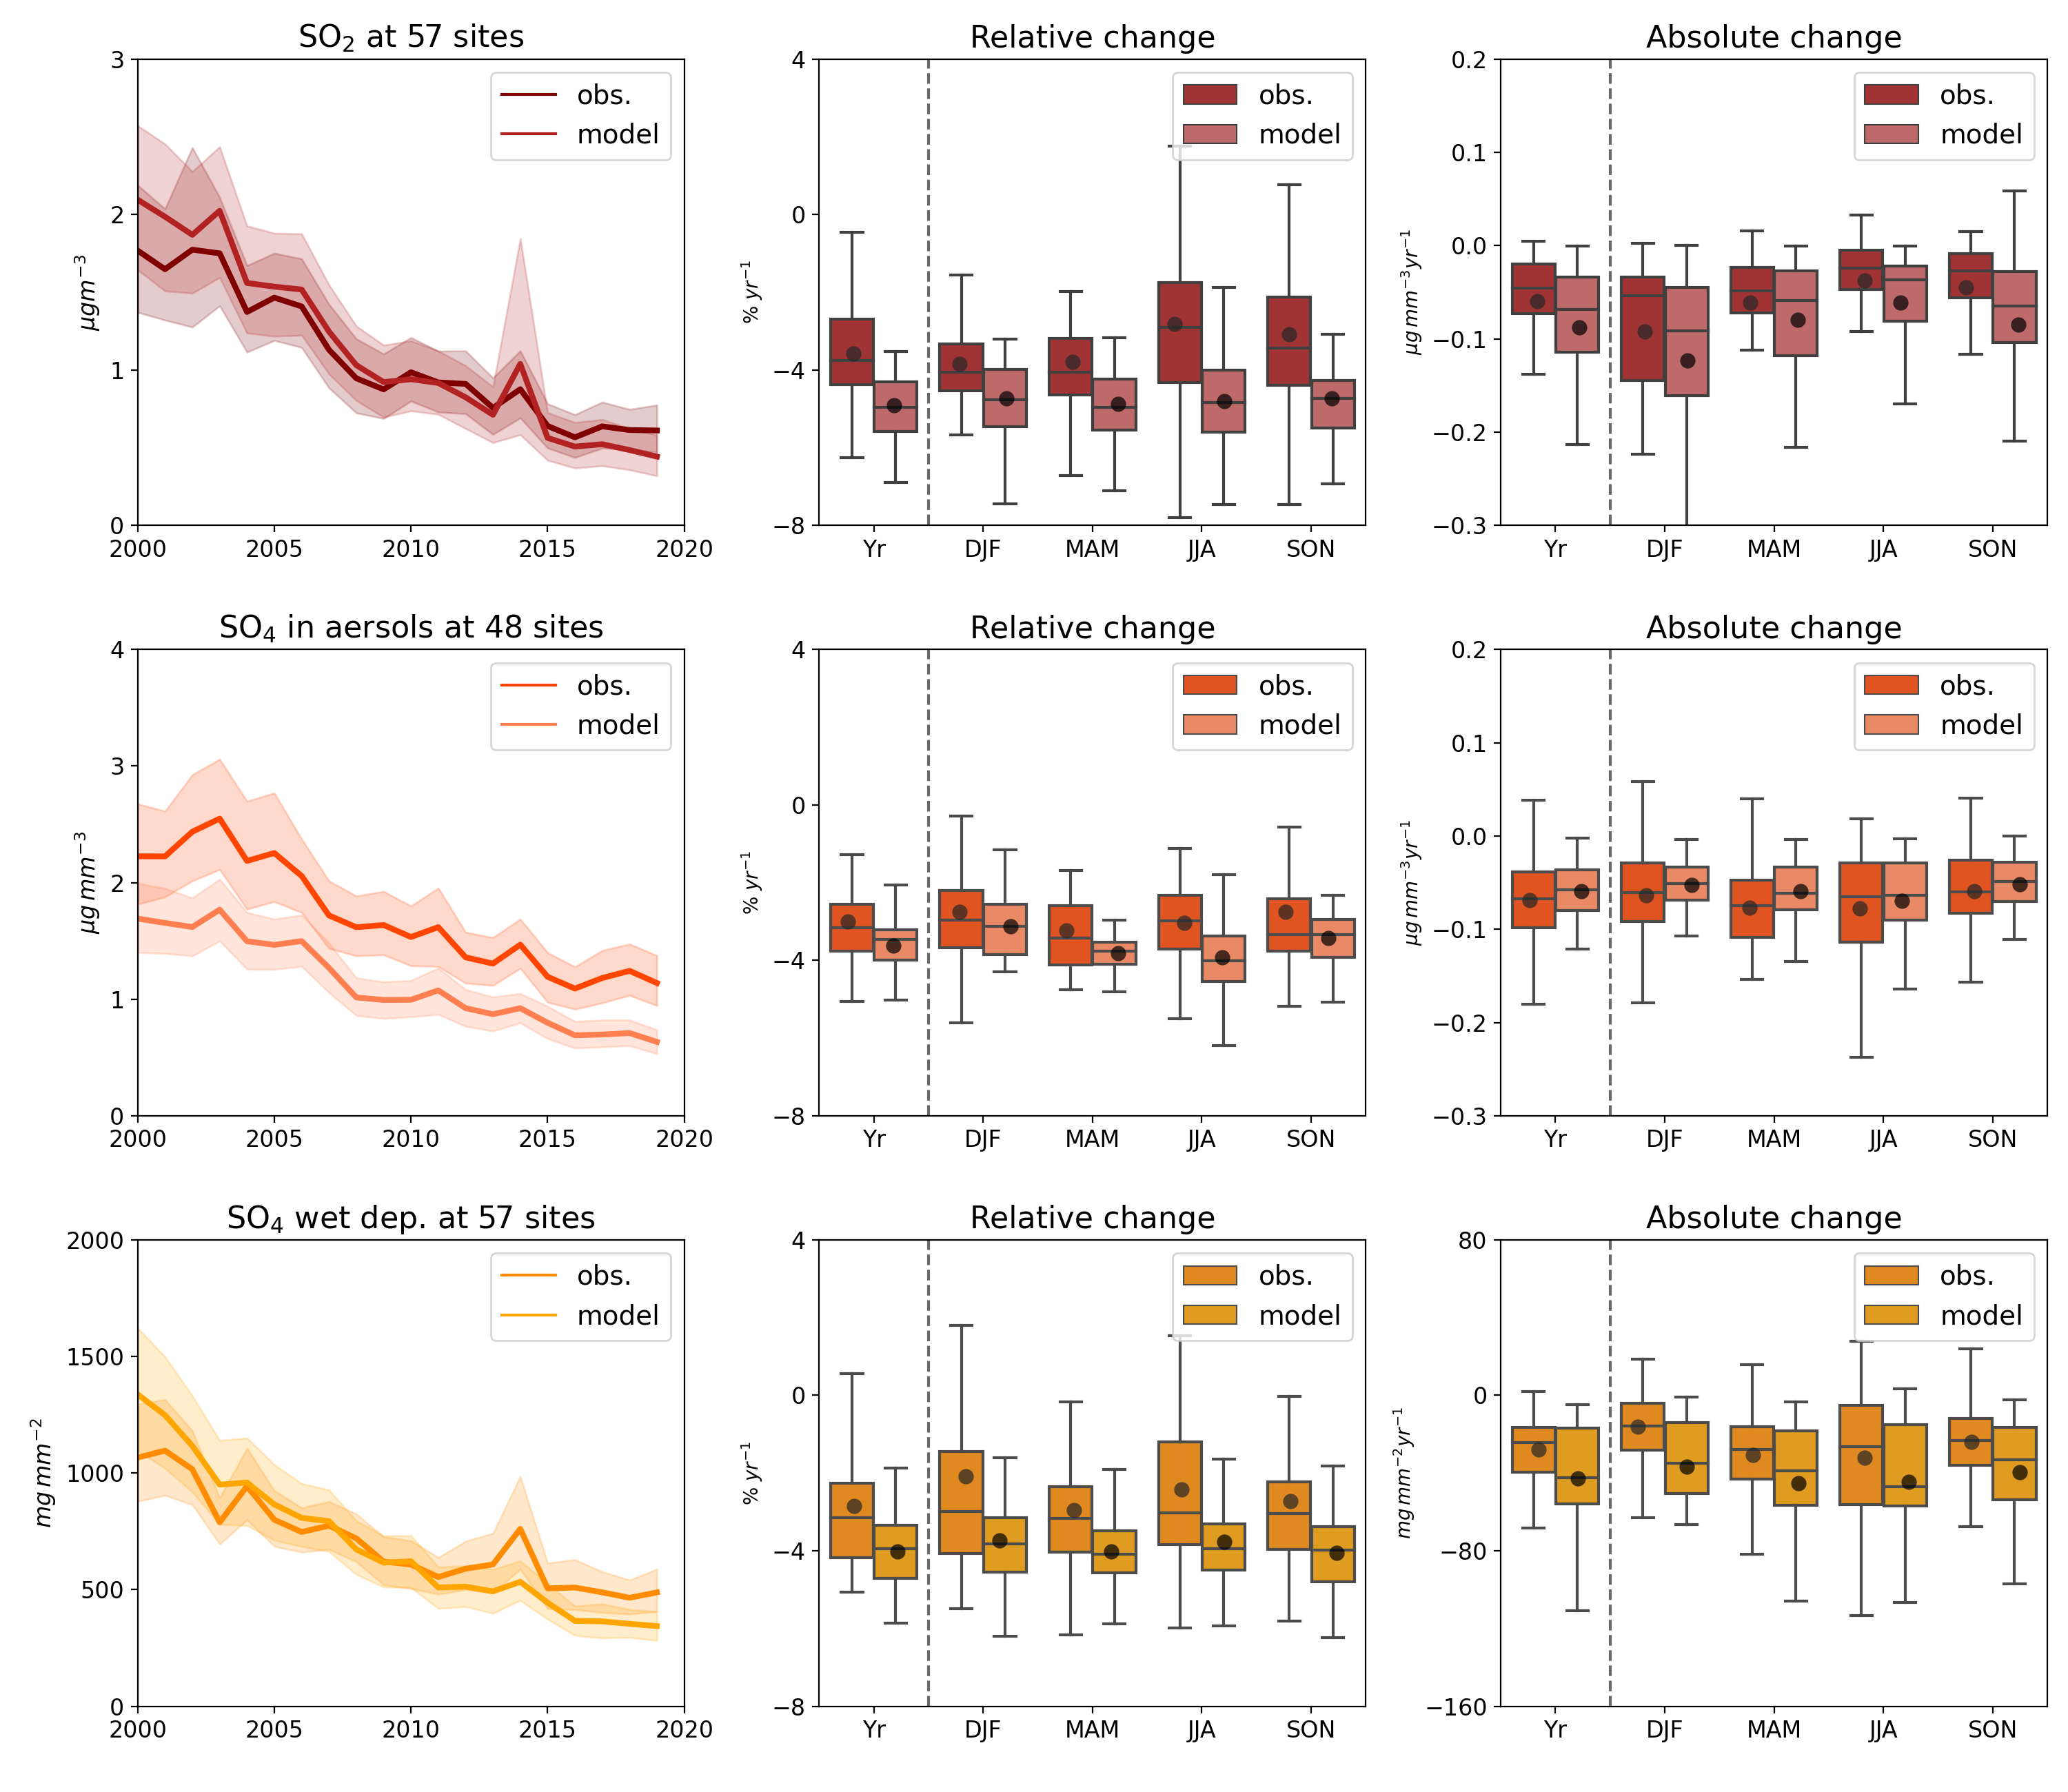
\includegraphics[width=0.74\paperwidth]{FIGS_TRENDS/sulfur_trends.png}
	\caption{\label{fig:SOx_trends}Trends in sulfur components from 2010-2019 for EMEP observations and model. The solid line in the trend plots indicate the average annual mean concentrations for all the sites and the shaded area the 95 \% confidence interval. The box plot represent the 50,25,75 percentiles and the whiskers lie within the 1.5 inter-quartile ranges for the trends of all the sites, including those with not significant trends. In addition, the mean trends are indicated with black circles and the trend in SOx emission is indicated in the plot of \soii with secondary y-axes}
\end{figure}

\begin{figure} [h]
  \centering{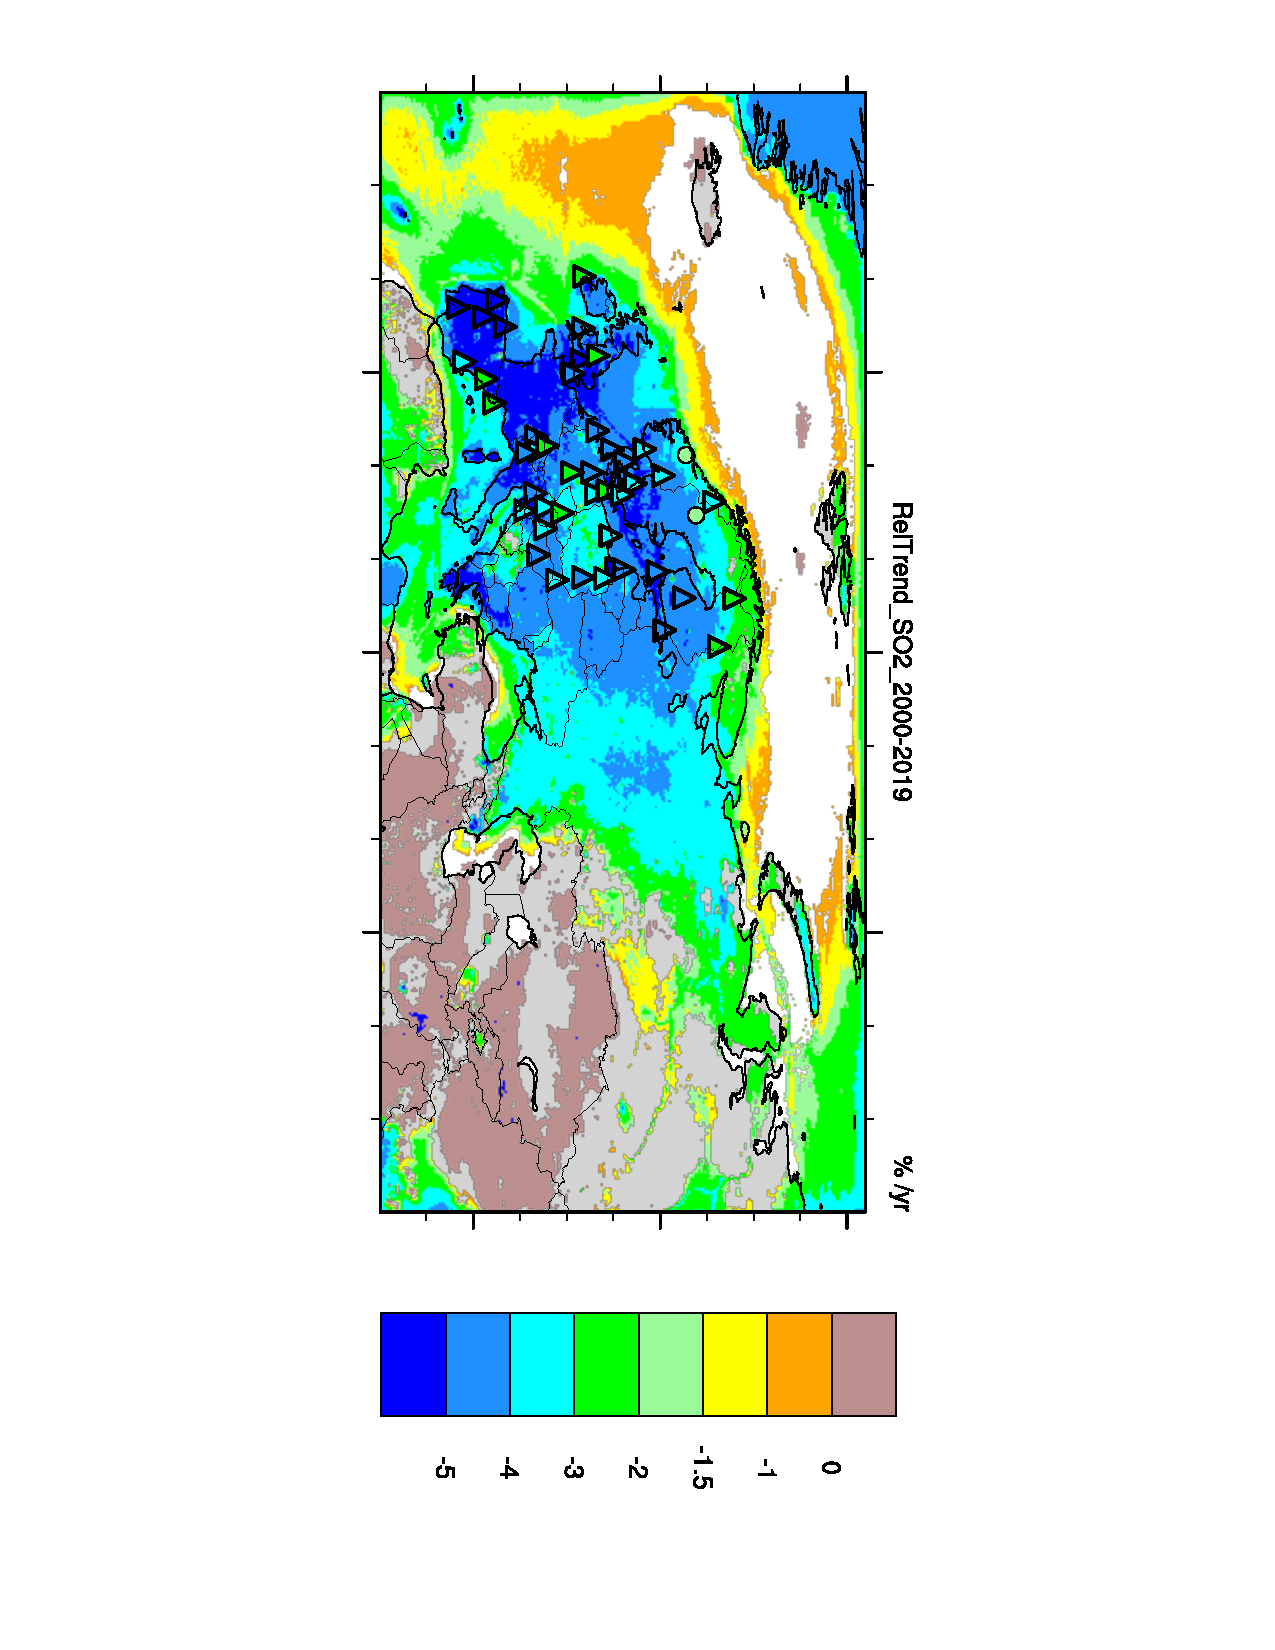
\includegraphics[clip=,angle=90,height=6.1cm,viewport=175 67 448 754]{FIGS_TRENDS/RelTrend_SO2_2000-2019_Perc.pdf}}\\
%  \vspace{0.5cm}
  \centering{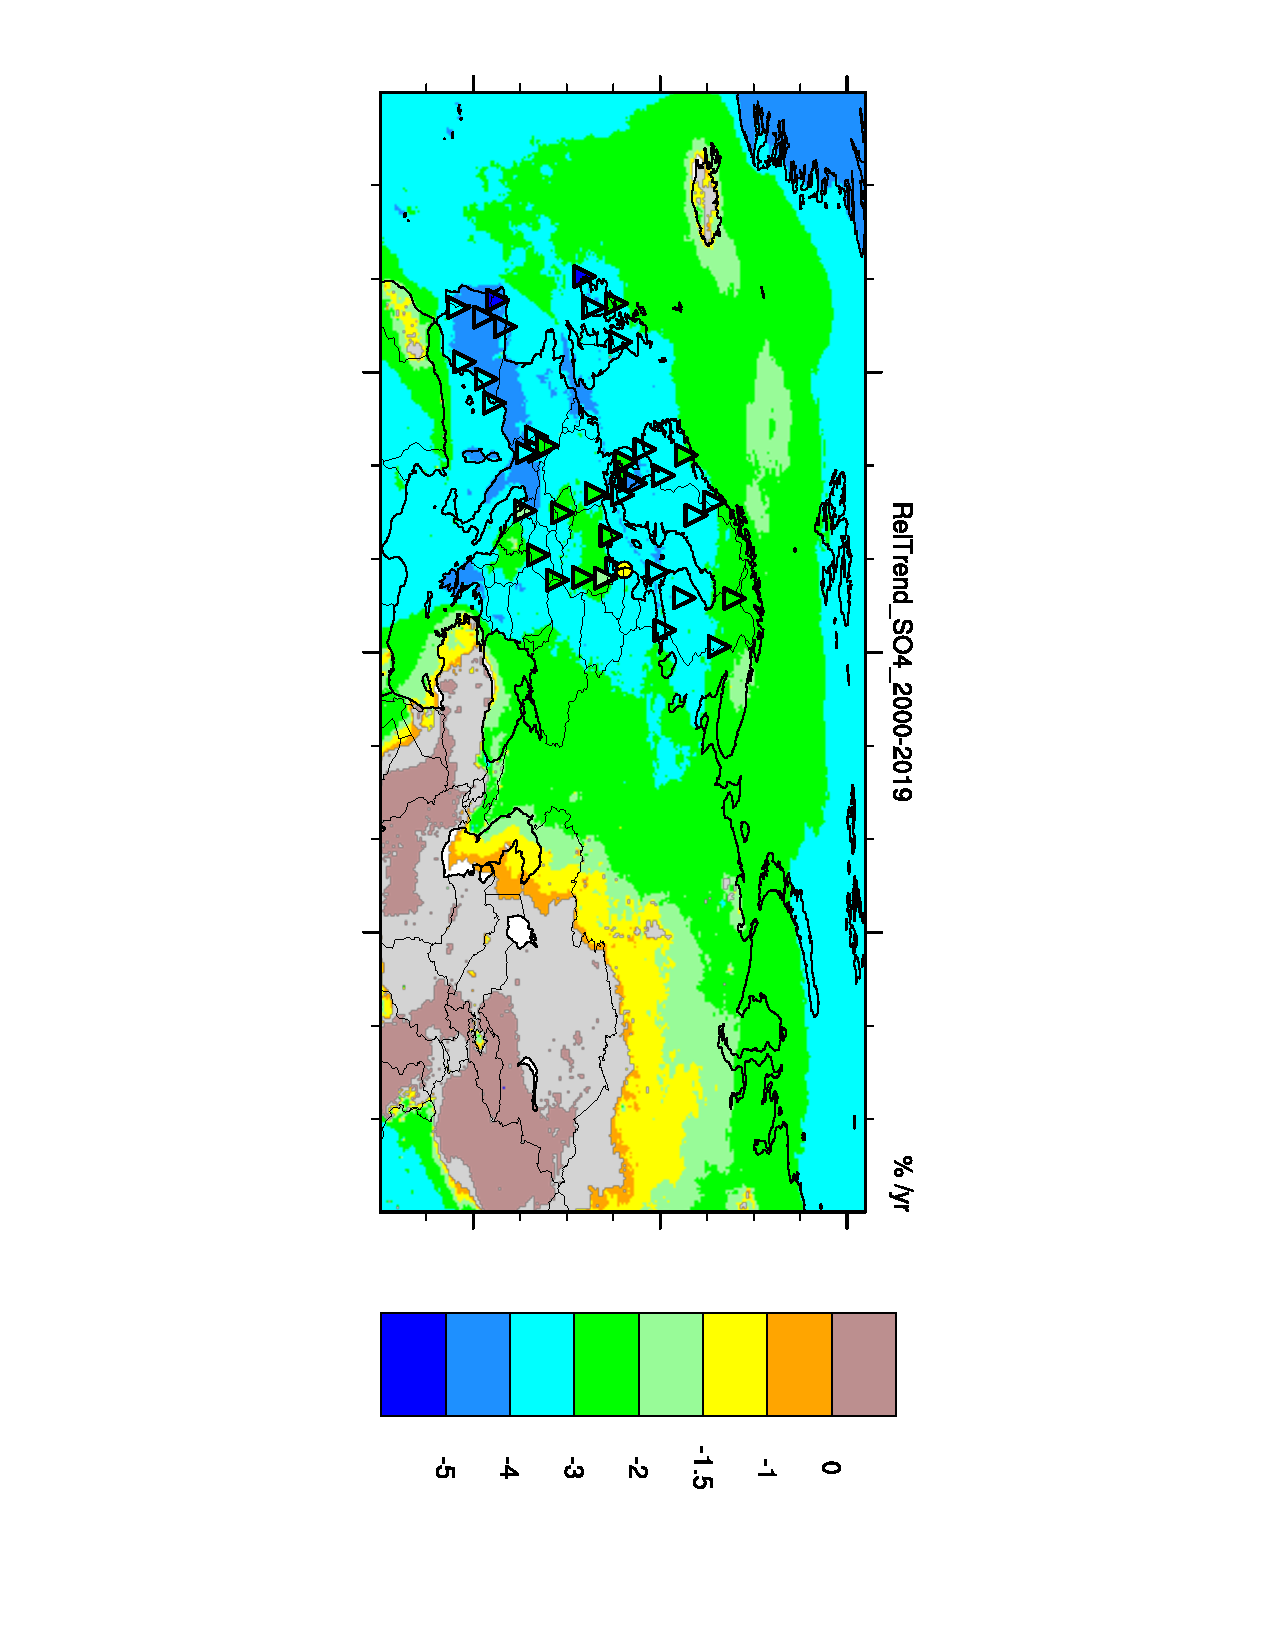
\includegraphics[clip=,angle=90,height=6.1cm,viewport=175 67 448 754]{FIGS_TRENDS/RelTrend_SO4_2000-2019_Perc.pdf}}
  %  \vspace{0.5cm}
  \centering{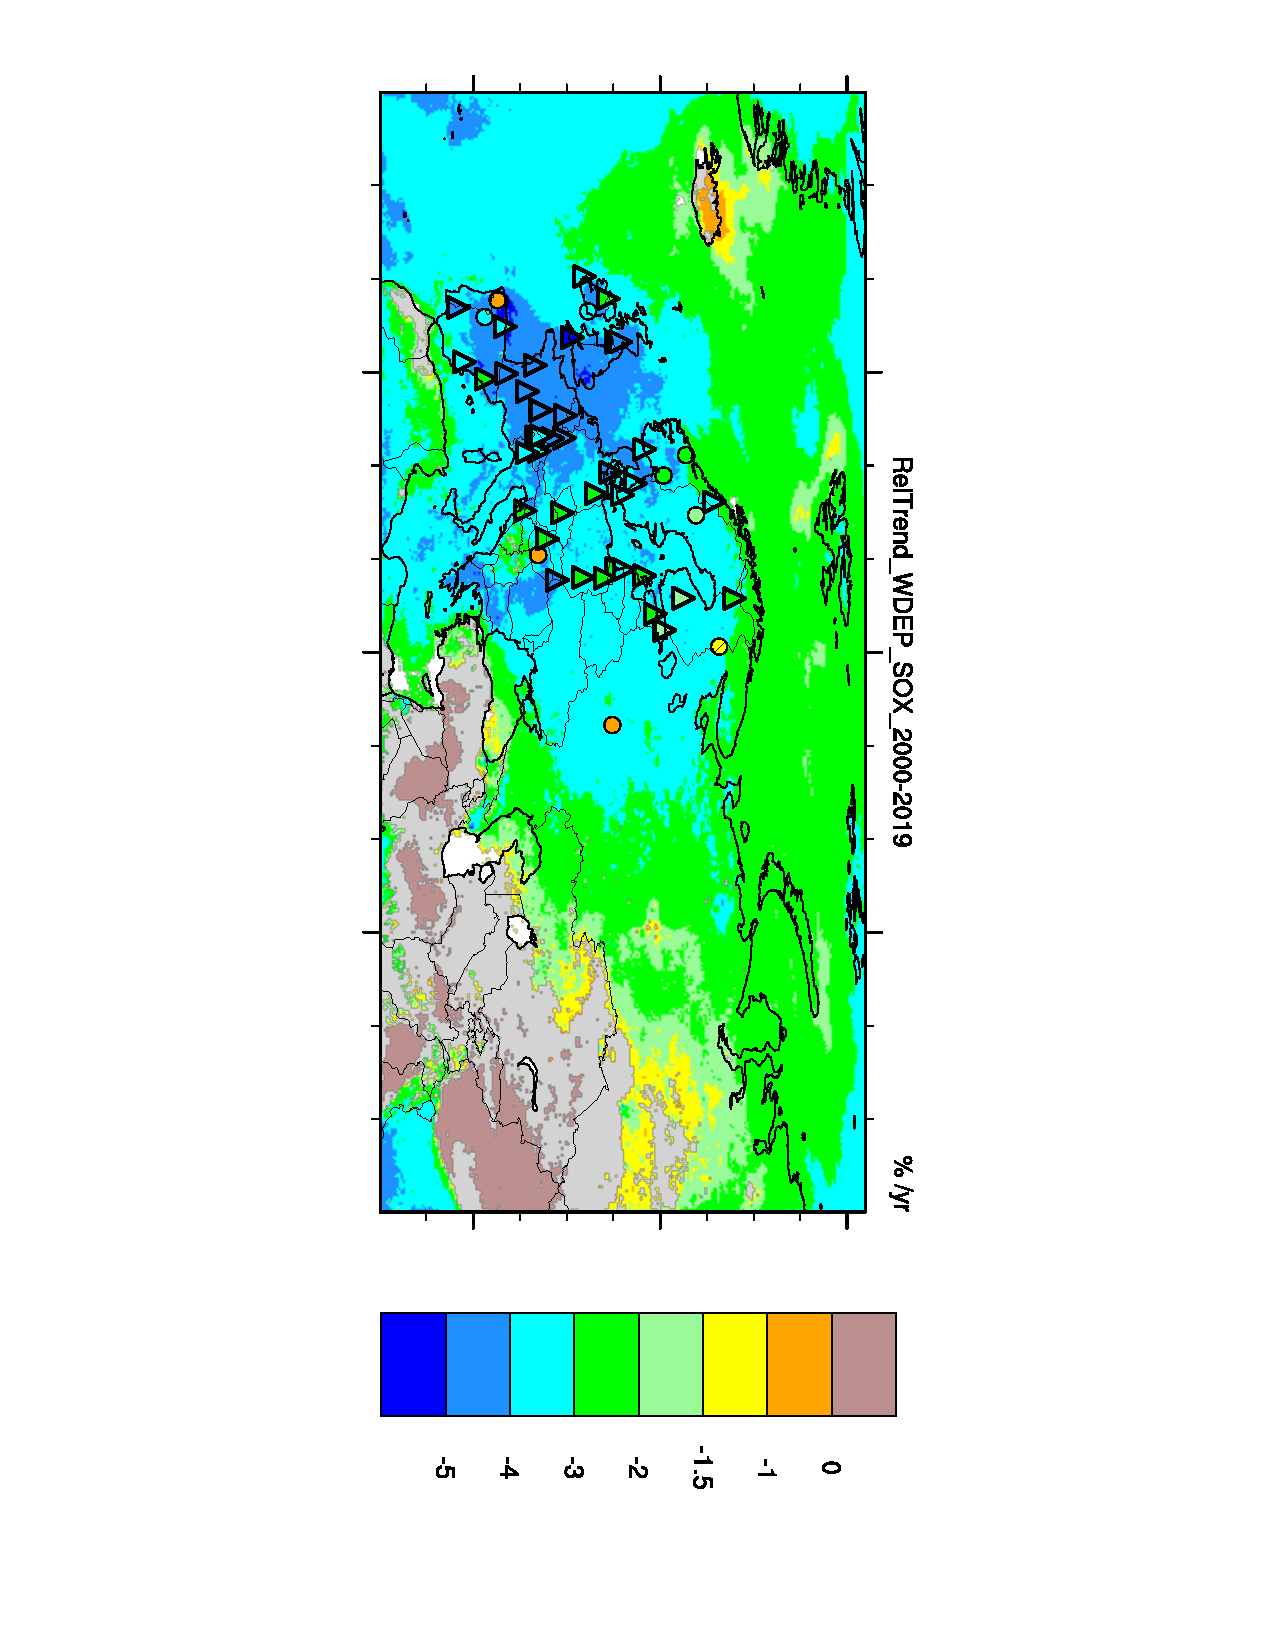
\includegraphics[clip=,angle=90,height=6.1cm,viewport=175 67 448 754]{FIGS_TRENDS/RelTrend_WDEP_SOX_2000-2019_Perc.pdf}}
\caption{Relative trends for \soii, \soiv in aerosols and wet deposition of \soiv in the period of 2000-2019: EMEP modelled -- coloured contours (grey/white means non-significant trends) and observed - coloured triangles (significant) and circles (non-significant).}
\label{fig:Strends_map}
\end{figure}



\begin{table}[h]
\caption{\label{tab:so2_stat} Absolute and relative change and corresponding 95\% confidence intervals in observed and modelled annual and seasonal aggregated \soii concentrations for the different time periods.The number of sites with a significant outcome is provided}
\begin{center}
\scalebox{0.65}{%
\begin{tabular}{ll|ccc|cccc|cccc}
\toprule
          &        & \multicolumn{3}{c}{Number of sites} & \multicolumn{4}{c}{Absolute change (\ug $yr^{-1})$} & \multicolumn{4}{c}{Relative change (\% $yr^{-1}$)} \\
Period & Seasons &           total & sign.(obs.) & sign.(mod.) &                    obs. &          conf.interval &  mod. &          conf.interval &                     obs. &         conf.interval &  mod. &        conf.interval \\
\midrule
2000-2019 & all &              48 &          46 &          48 &                  -0.068 &  (-0.085, -0.051) & -0.088 &  (-0.109, -0.067) &                    -3.88 &  (-4.23, -3.53) & -5.10 &  (-5.39, -4.81) \\
          & winter &              50 &          45 &          49 &                  -0.102 &  (-0.127, -0.076) & -0.124 &  (-0.153, -0.095) &                    -4.08 &   (-4.36, -3.8) & -4.94 &  (-5.22, -4.65) \\
          & spring &              48 &          45 &          48 &                  -0.070 &  (-0.086, -0.053) & -0.081 &  (-0.101, -0.061) &                    -4.15 &  (-4.45, -3.85) & -5.09 &  (-5.35, -4.84) \\
          & summer &              48 &          33 &          48 &                  -0.043 &  (-0.057, -0.029) & -0.060 &  (-0.078, -0.041) &                    -3.01 &  (-3.59, -2.43) & -4.94 &   (-5.3, -4.58) \\
          & autumn &              48 &          36 &          47 &                  -0.051 &  (-0.066, -0.035) & -0.086 &  (-0.107, -0.064) &                    -3.55 &  (-3.94, -3.15) & -5.02 &   (-5.3, -4.75) \\
2005-2019 & all &              57 &          41 &          54 &                  -0.055 &  (-0.068, -0.041) & -0.067 &   (-0.084, -0.05) &                    -4.27 &  (-4.72, -3.83) & -5.26 &   (-5.6, -4.93) \\
2010-2019 & all &              60 &          36 &          42 &                  -0.050 &  (-0.062, -0.037) & -0.056 &  (-0.072, -0.041) &                    -4.81 &  (-5.94, -3.69) & -6.39 &  (-7.15, -5.63) \\
2000-2010 & all &              66 &          30 &          58 &                  -0.079 &  (-0.103, -0.054) & -0.117 &  (-0.142, -0.091) &                    -3.52 &  (-4.31, -2.73) & -5.39 &  (-5.93, -4.84) \\
\bottomrule
\end{tabular}}
\end{center}
\end{table}

\begin{table}[h]
\caption{\label{tab:so4pm_stat} Absolute and relative change and corresponding 95\% confidence intervals in observed and modelled annual and seasonal aggregated \soiv concentrations for the different time periods.The number of sites with a significant outcome is provided}
\begin{center}
\scalebox{0.65}{%
\begin{tabular}{ll|ccc|cccc|cccc}
\toprule
          &        & \multicolumn{3}{c}{Number of sites} & \multicolumn{4}{c}{Absolute change (\ug $yr^{-1})$} & \multicolumn{4}{c}{Relative change (\% $yr^{-1}$)} \\
Period & Seasons &           total & sign.(obs.) & sign.(mod.) &                    obs. &          conf.interval &  mod. &          conf.interval &                     obs. &         conf.interval &  mod. &        conf.interval \\
\midrule
2000-2019 & all &              39 &          38 &          39 &                  -0.074 &  (-0.087, -0.062) & -0.065 &  (-0.076, -0.053) &                    -3.20 &  (-3.46, -2.93) & -3.81 &  (-4.04, -3.58) \\
          & winter &              40 &          29 &          34 &                  -0.064 &   (-0.08, -0.049) & -0.056 &  (-0.066, -0.046) &                    -2.75 &  (-3.22, -2.28) & -3.21 &  (-3.44, -2.97) \\
          & spring &              38 &          36 &          38 &                  -0.085 &  (-0.098, -0.072) & -0.065 &  (-0.075, -0.055) &                    -3.46 &  (-3.72, -3.19) & -4.03 &  (-4.21, -3.84) \\
          & summer &              38 &          36 &          38 &                  -0.082 &  (-0.102, -0.063) & -0.078 &  (-0.097, -0.059) &                    -3.15 &  (-3.46, -2.85) & -4.20 &   (-4.5, -3.91) \\
          & autumn &              37 &          34 &          37 &                  -0.062 &   (-0.073, -0.05) & -0.057 &  (-0.067, -0.046) &                    -3.08 &   (-3.4, -2.76) & -3.59 &  (-3.81, -3.38) \\
2005-2019 & all &              43 &          35 &          42 &                  -0.067 &  (-0.079, -0.055) & -0.054 &  (-0.063, -0.046) &                    -3.48 &  (-3.88, -3.09) & -4.01 &  (-4.25, -3.77) \\
2010-2019 & all &              46 &          20 &          32 &                  -0.053 &  (-0.068, -0.038) & -0.044 &  (-0.055, -0.034) &                    -3.43 &  (-4.11, -2.75) & -4.26 &  (-4.91, -3.62) \\
2000-2010 & all &              54 &          15 &          43 &                  -0.068 &  (-0.085, -0.051) & -0.094 &  (-0.109, -0.079) &                    -2.51 &  (-2.95, -2.07) & -4.19 &  (-4.52, -3.86) \\
\bottomrule
\end{tabular}}
\end{center}
\end{table}

\begin{table}[h]
\caption{\label{tab:so4dep_stat} Absolute and relative change and corresponding 95\%  confidence intervals in observed and modelled annual and seasonal aggregated wet deposition of sulfate for the different time periods.The number of sites with a significant outcome is provided}
\begin{center}
\scalebox{0.65}{%
\begin{tabular}{ll|ccc|cccc|cccc}
\toprule
          &        & \multicolumn{3}{c}{Number of sites} & \multicolumn{4}{c}{Absolute change (\ug $m^{2} yr^{-1}$)} & \multicolumn{4}{c}{Relative change (\% $yr^{-1}$)} \\
Period & Seasons &           total & sign.(obs.) & sign.(mod.) &                    obs. &          conf.interval &  mod. &          conf.interval &                     obs. &         conf.interval &  mod. &        conf.interval \\
\midrule
2000-2019 & all &              49 &          40 &          49 &                   -29.5 &  (-34.8, -24.2) & -48.1 &   (-56.9, -39.4) &                    -3.14 &  (-3.46, -2.82) & -4.27 &   (-4.5, -4.04) \\
          & winter &              47 &          25 &          44 &                   -19.5 &  (-24.5, -14.5) & -41.4 &   (-49.5, -33.3) &                    -2.87 &   (-3.34, -2.4) & -3.97 &  (-4.21, -3.73) \\
          & spring &              45 &          30 &          45 &                   -32.7 &  (-39.1, -26.2) & -49.2 &   (-59.7, -38.6) &                    -3.23 &   (-3.6, -2.86) & -4.19 &  (-4.41, -3.98) \\
          & summer &              47 &          31 &          45 &                   -36.5 &  (-44.5, -28.5) & -52.6 &   (-63.0, -42.2) &                    -2.95 &  (-3.35, -2.54) & -4.20 &  (-4.46, -3.94) \\
          & autumn &              46 &          27 &          42 &                   -26.7 &  (-32.3, -21.1) & -45.0 &   (-54.6, -35.5) &                    -3.00 &  (-3.49, -2.51) & -4.25 &  (-4.52, -3.99) \\
2005-2019 & all &              53 &          30 &          50 &                   -22.9 &  (-27.9, -17.9) & -36.3 &   (-42.4, -30.2) &                    -2.87 &  (-3.51, -2.22) & -4.53 &  (-4.79, -4.27) \\
2010-2019 & all &              60 &          15 &          40 &                   -20.9 &  (-27.1, -14.6) & -34.0 &   (-40.6, -27.3) &                    -2.86 &  (-3.78, -1.93) & -5.08 &  (-5.56, -4.59) \\
2000-2010 & all &              54 &          28 &          44 &                   -46.9 &  (-56.6, -37.1) & -68.5 &   (-81.4, -55.7) &                    -4.44 &  (-5.15, -3.74) & -5.29 &   (-5.68, -4.9) \\
\bottomrule
\end{tabular}}
\end{center}
\end{table}


\section{\label{sec:Trends_oxidised_nitrogen }Trends in oxidised nitrogen}

During the last decades, the total emissions of NO$_x$ declined significantly in Europe, followed by declining nitrogen dioxide concentrations, total nitrate (nitric acid plus particulate nitrate) in air and oxidized nitrogen wet deposition at EMEP background sites. This is found both for the EMEP MSC-W model calculations and for observations. Similar results have been presented in \citet{Theobald2019} for wet deposition of oxidized nitrogen for the 1990-2010 period and in \citet{Banzhaf2015} for total nitrate for 1990-2009. \citet{torseth2012} also find decreasing trends in nitrogen dioxide, total nitrate and nitrate in precipitations 1990-2009 in EMEP observations. A more recent study, analyzing the period 2000-2017 \citep{Colette2021} and including Airbase and most EMEP observations, also find decreasing trends in nitrogen dioxide.

Figure~\ref{fig:NOx_trends} shows an overview of the annual and seasonal trends in oxidised nitrogen compounds from 2000 to 2019. Tables~\ref{tab:no2_stat} to \ref{tab:no3dep_stat} show absolute and relative changes in the different oxidized nitrogen compounds.

From 2000-2019, the reductions have been on average -1.2\% yr$^{-1}$ for nitrogen dioxide concentrations at EMEP background sites (total -24\%). As NO$_2$ has a short lifetime, the trend in NO$_2$ is expected to reflect the trend in (local) emissions of NOx. During the 2000-2019 period, NO$_x$ emissions within the western EMEP domain (EU27+UK+EFTA countries), where the dominant part of the long term EMEP observations are situated, decreased by -48\%. EMEP/MSC-W model calculations follows the reported emission reductions closely (average reductions of -2.2\% yr$^{-1}$, or in total -42\% ). 
The agreement between the trends calculated from observations and from the model (and emissions) agree well for the last period (2010-2019), with trends around -2.3\% yr$^{-1}$, whilst the trend in the first period is substantially lower in the observations than in the model calculations (and emissions). From Figure~\ref{fig:NOx_trends} it can be seen that the agreement between observations and model calculations is excellent until around 2008, but that in the year 2009 and onwards the model (and emissions) is shifted down relative to the observations. Similar results have been found in \citep{Colette2021}.




The trends in wet deposition of oxidized nitrogen reflects the long range transported oxidized nitrogen (e.g. NO$_x$ that has been converted to nitric acid and particulate nitrate and then washed out by rain) and is less sensitive to local changes. Also the trends for wet deposition of nitrate are lower in the observations than in the model calculations (and emissions of NO$_x$) for the 2000-2019 period. Whilst the average trend in observations is -1.4\% yr$^{-1}$ (total of -26\%), the model calculates the trend at the same sites to be -2.1 \% yr$^{-1}$ (total of -40\%), close to the trends in emissions from the western EMEP domain (-48\%). The difference between the trend in observations are largest during the first period, similar to the results for NO$_2$. However, the model overestimates nitrate wet deposition somewhat up to around 2010, and are then shifted downward and in very good agreement with observations for the years after. Note that the number of sites with significant trends for the shorter periods are small, and thus the results encumbered with more uncertainty.

For particulate nitrate, nitric acid and their sum the results are more complex. The number of sites are few (especially for nitric acid, with only 6 sites), the coverage of Europe more scattered and the quality of the measurements is worse. 

The modelled trends for 2000 to 2019 are all around -2 to -2.3\% per year for particulate nitrate, nitric acid and their sum - aligned with the results of NO$_2$, wet deposition of oxidized nitrogen and the emissions. The observations show a somewhat smaller negative trend of around -1.6\% yr$^{-1}$ for the sum and around -2\% yr$^{-1}$ both for particulate nitrate and nitric acid. For the shorter periods, the number of sites with significant trends are very small, both in the model calculations and the observations, and thus the results more uncertain.
However, for all the three observations, the trend in the first period (2000-2010) is smaller than the trend in the second period, whilst the model show a rather similar trend for the sum, and larger trends in the first period for the separate components.

In Figure~\ref{fig:OXNtrends}, the trends for the individual sites are visualized on a map on top of the EMEP MSC-W model calculations. For NO$_2$ and wet deposition of oxidized nitrogen, the trends in the observations on the eastern part of the domain are smaller and to a larger extent non significant, whilst the trends in the EMEP MSC-W model calculations are in general larger and more often significant. The reasons for these discrepancies are not clear, but could be related to problems/inaccuracies in emission reporting and their trends, processes that are not (well enough) taken into account or in the observations themselves.

In summary we find that oxidized nitrogen in air and precipitation has been decreasing since 2000. However, the decrease in the observations (-24\% for \noii and -26\% for wet deposition of oxidized nitrogen) are smaller than in model calculations (-42\% for \noii and -40\% for wet deposition of oxidized nitrogen) and emissions (-48\% for EU27+UK+EFTA). 

\begin{figure}[h]
	\centering
	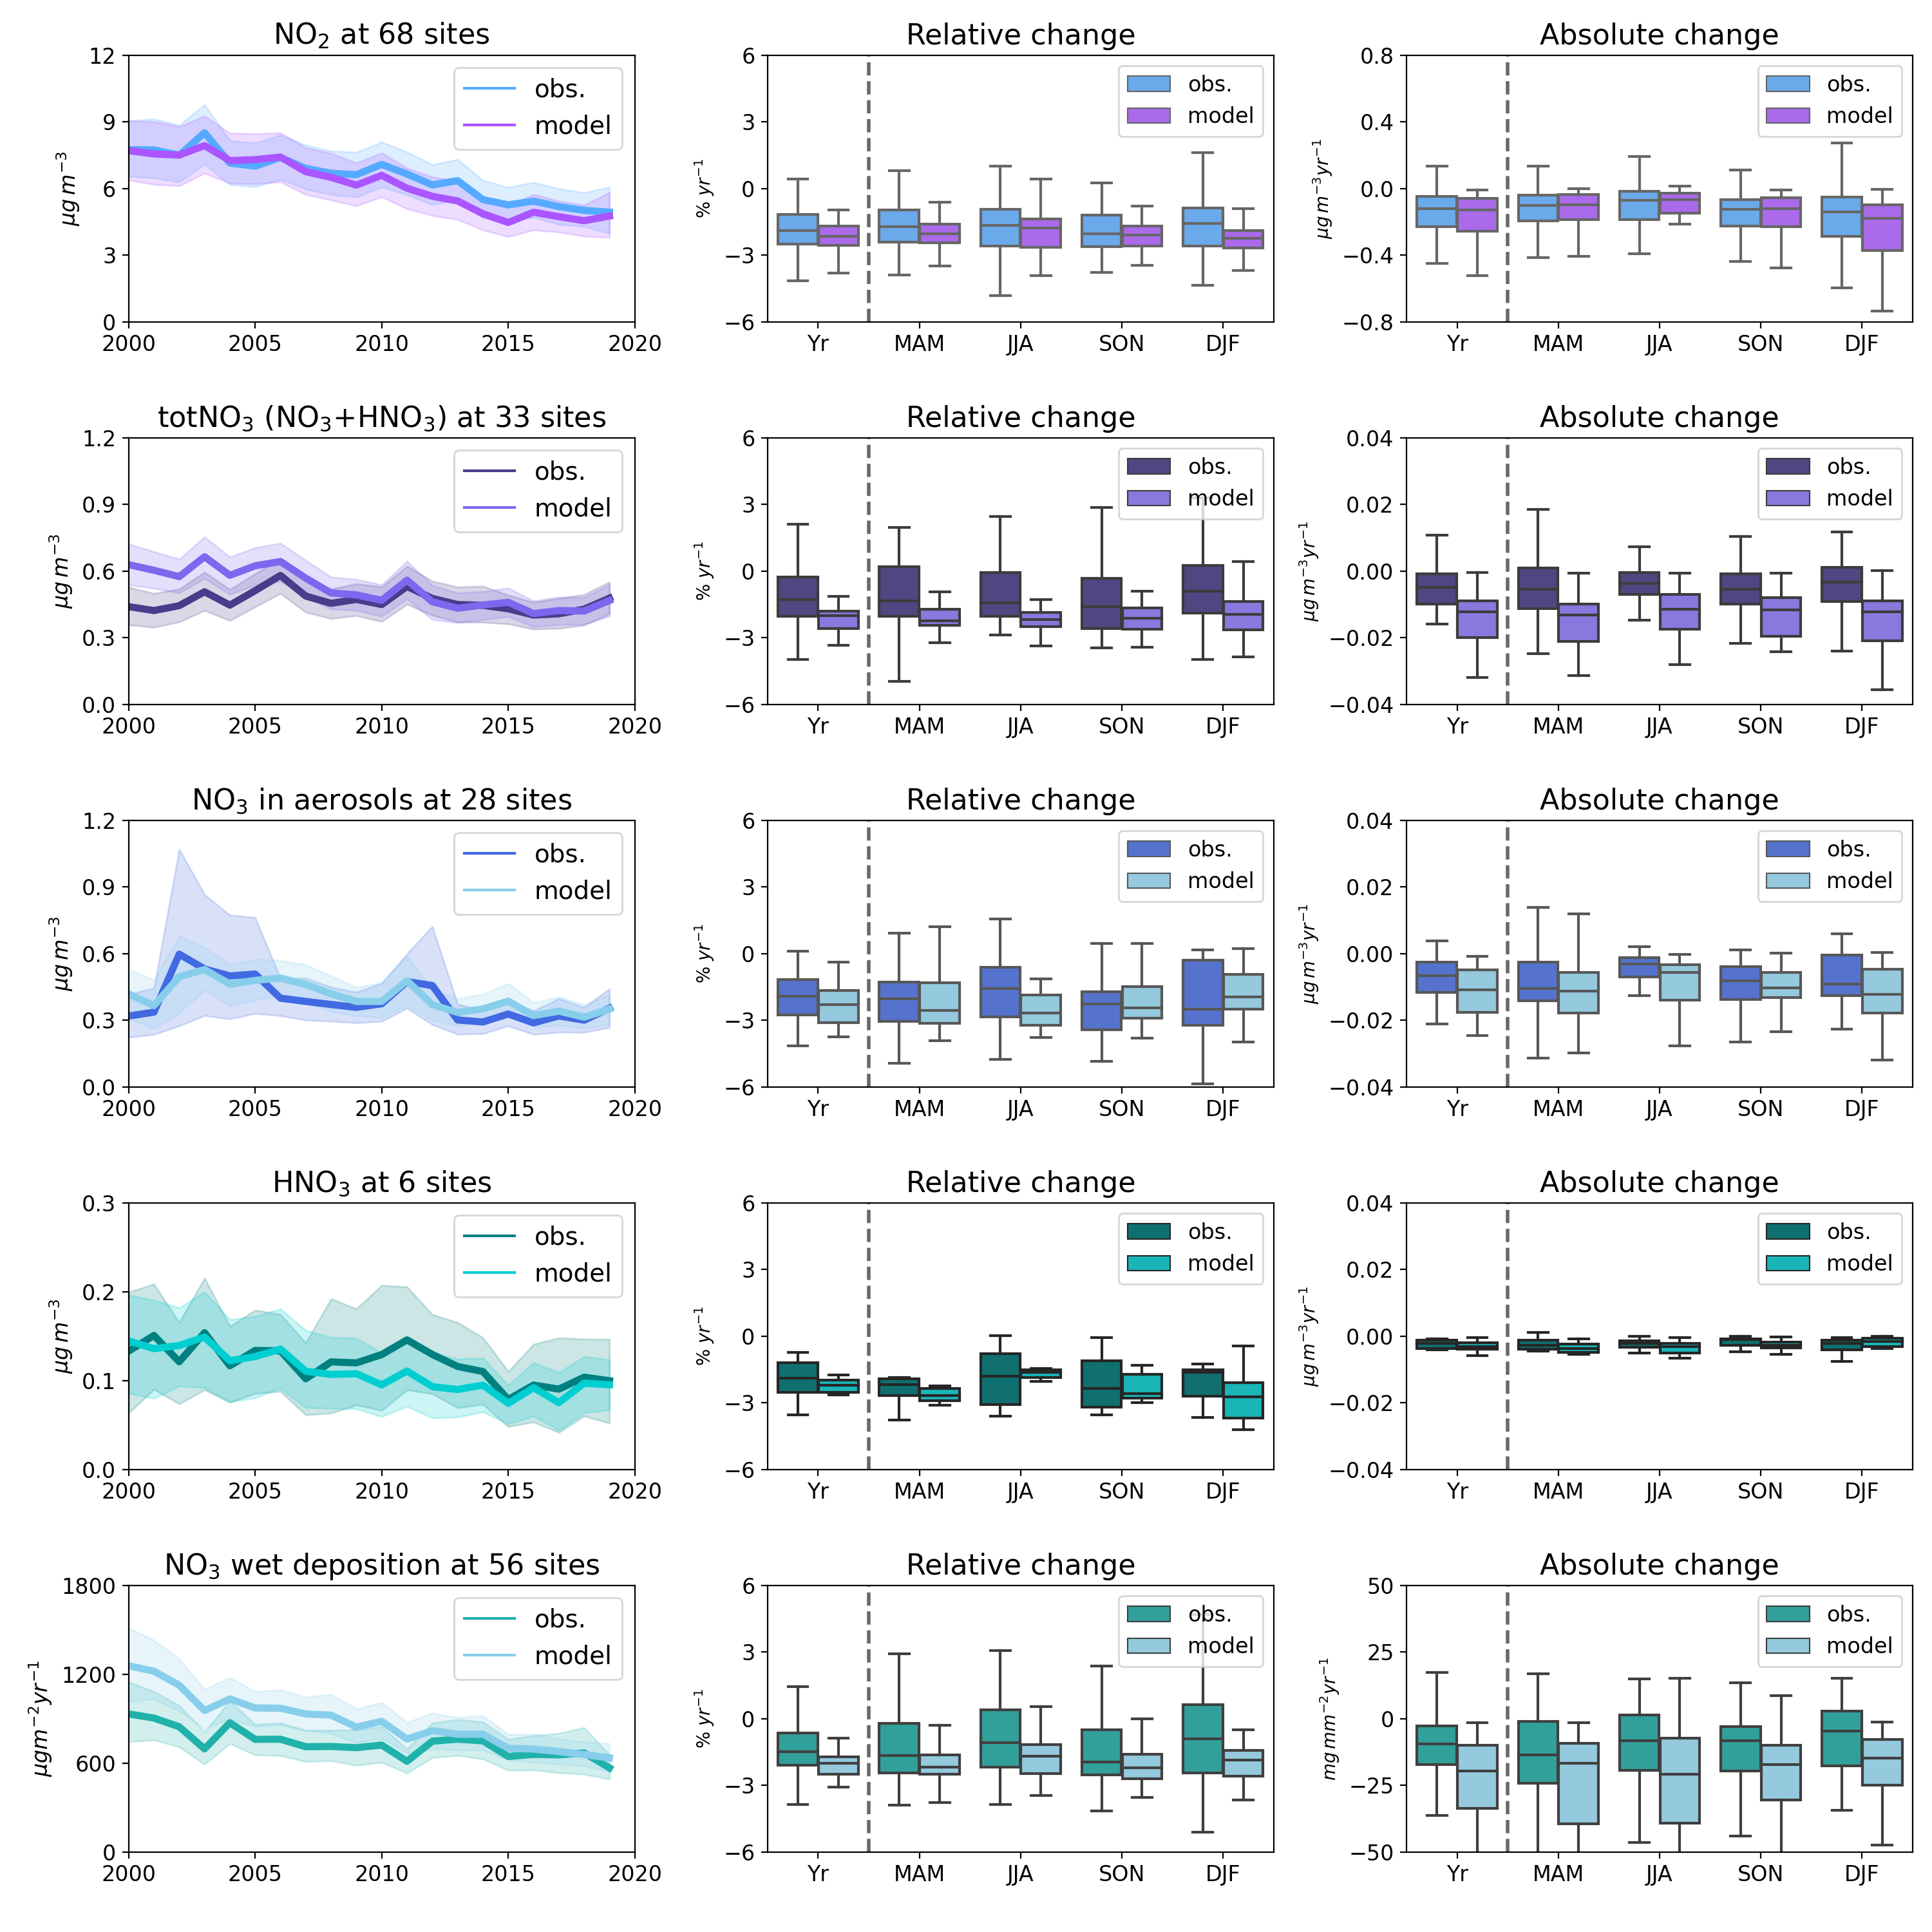
\includegraphics[width=0.74\paperwidth]{FIGS_TRENDS/Nox_trends.png}
	\caption{\label{fig:NOx_trends}Trends in oxidised nitrogen compounds from 2010-2019 for EMEP observations and model. The solid line in the trend plots indicate the average annual mean concentrations for all the sites and the shaded area the 95 \% confidence interval. The box plot represent the 50,25,75 percentiles and the whiskers lie within the 1.5 inter-quartile ranges for the trends of all the sites, including those with not significant trends. In addition, the mean trends are indicated with black circles and the trend in NOx emission is indicated in the plot of \noii with secondary y-axes}
\end{figure}

\begin{figure}[h]
  \centering{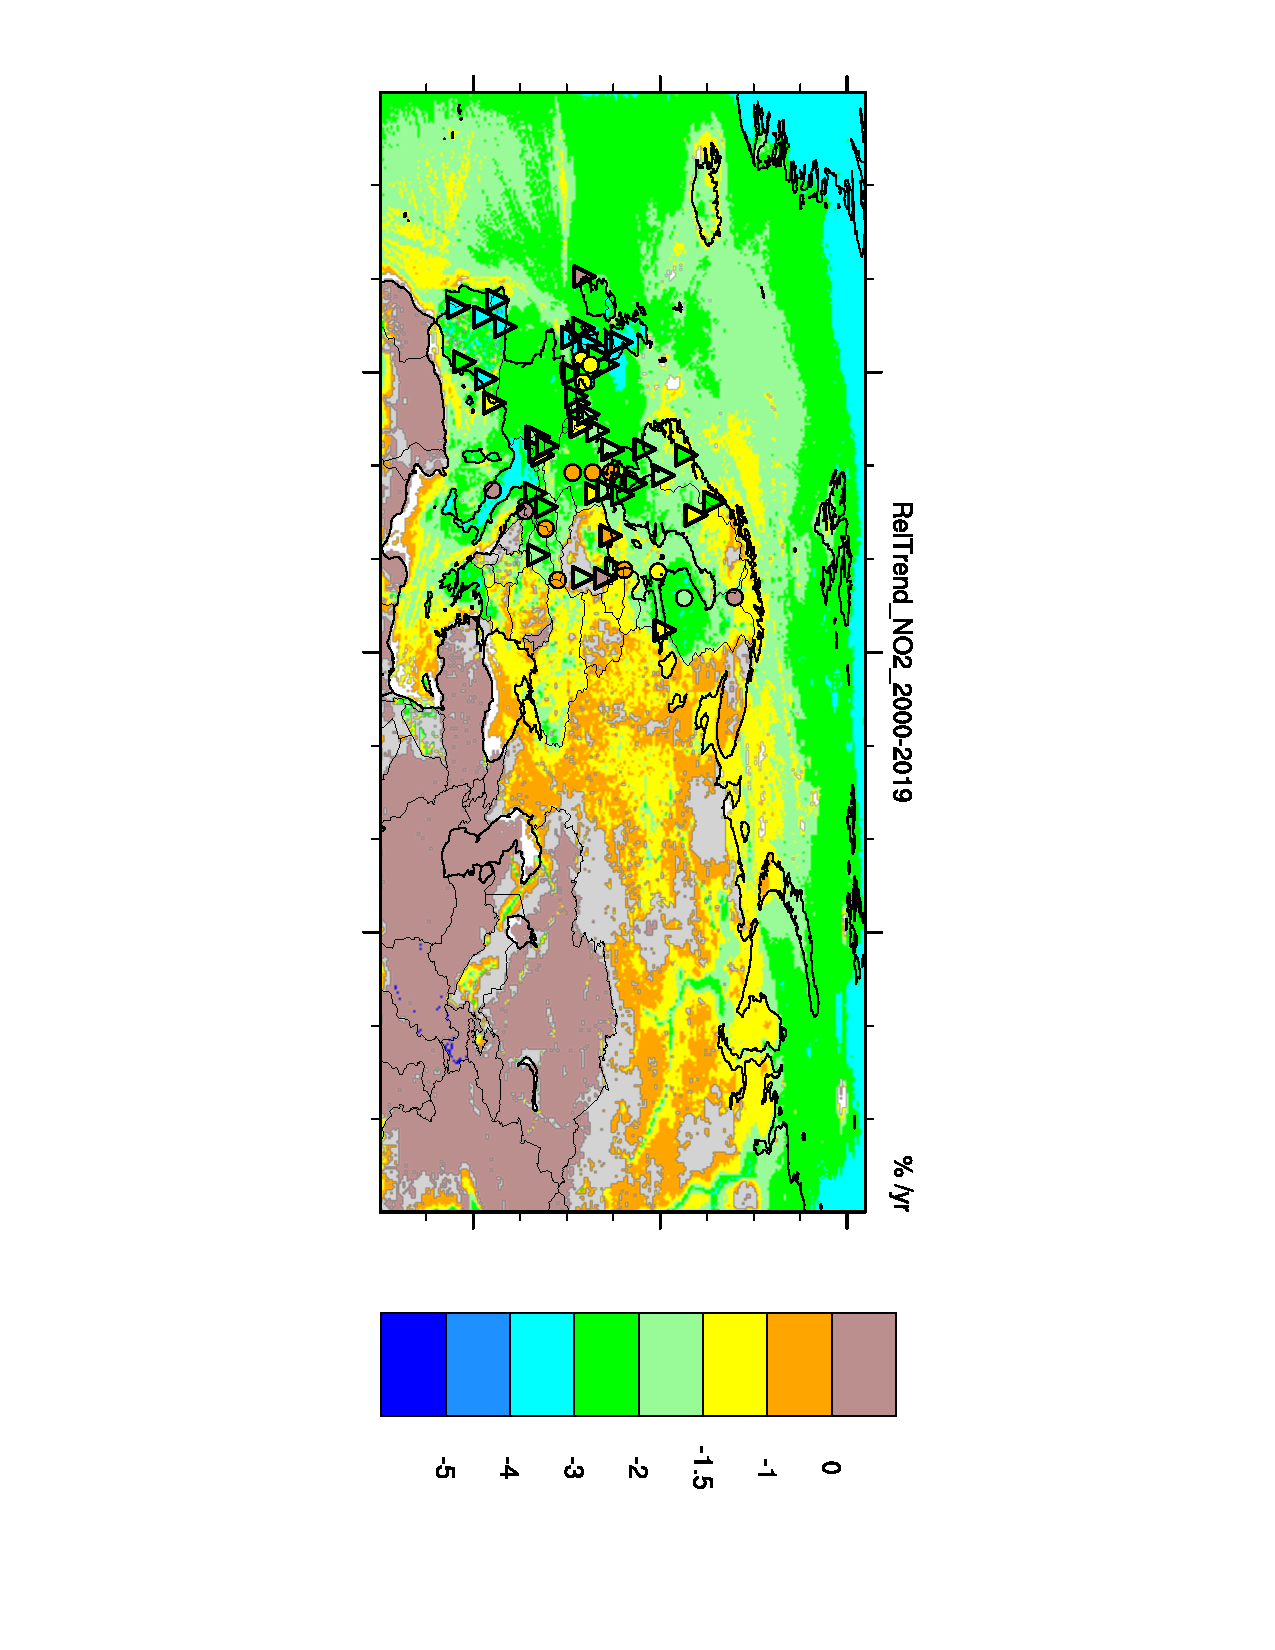
\includegraphics[clip=,angle=90,height=6.1cm,viewport=175 67 448 754]{FIGS_TRENDS/RelTrend_NO2_2000-2019_Perc.pdf}}
%  \vspace{0.5cm}
  \centering{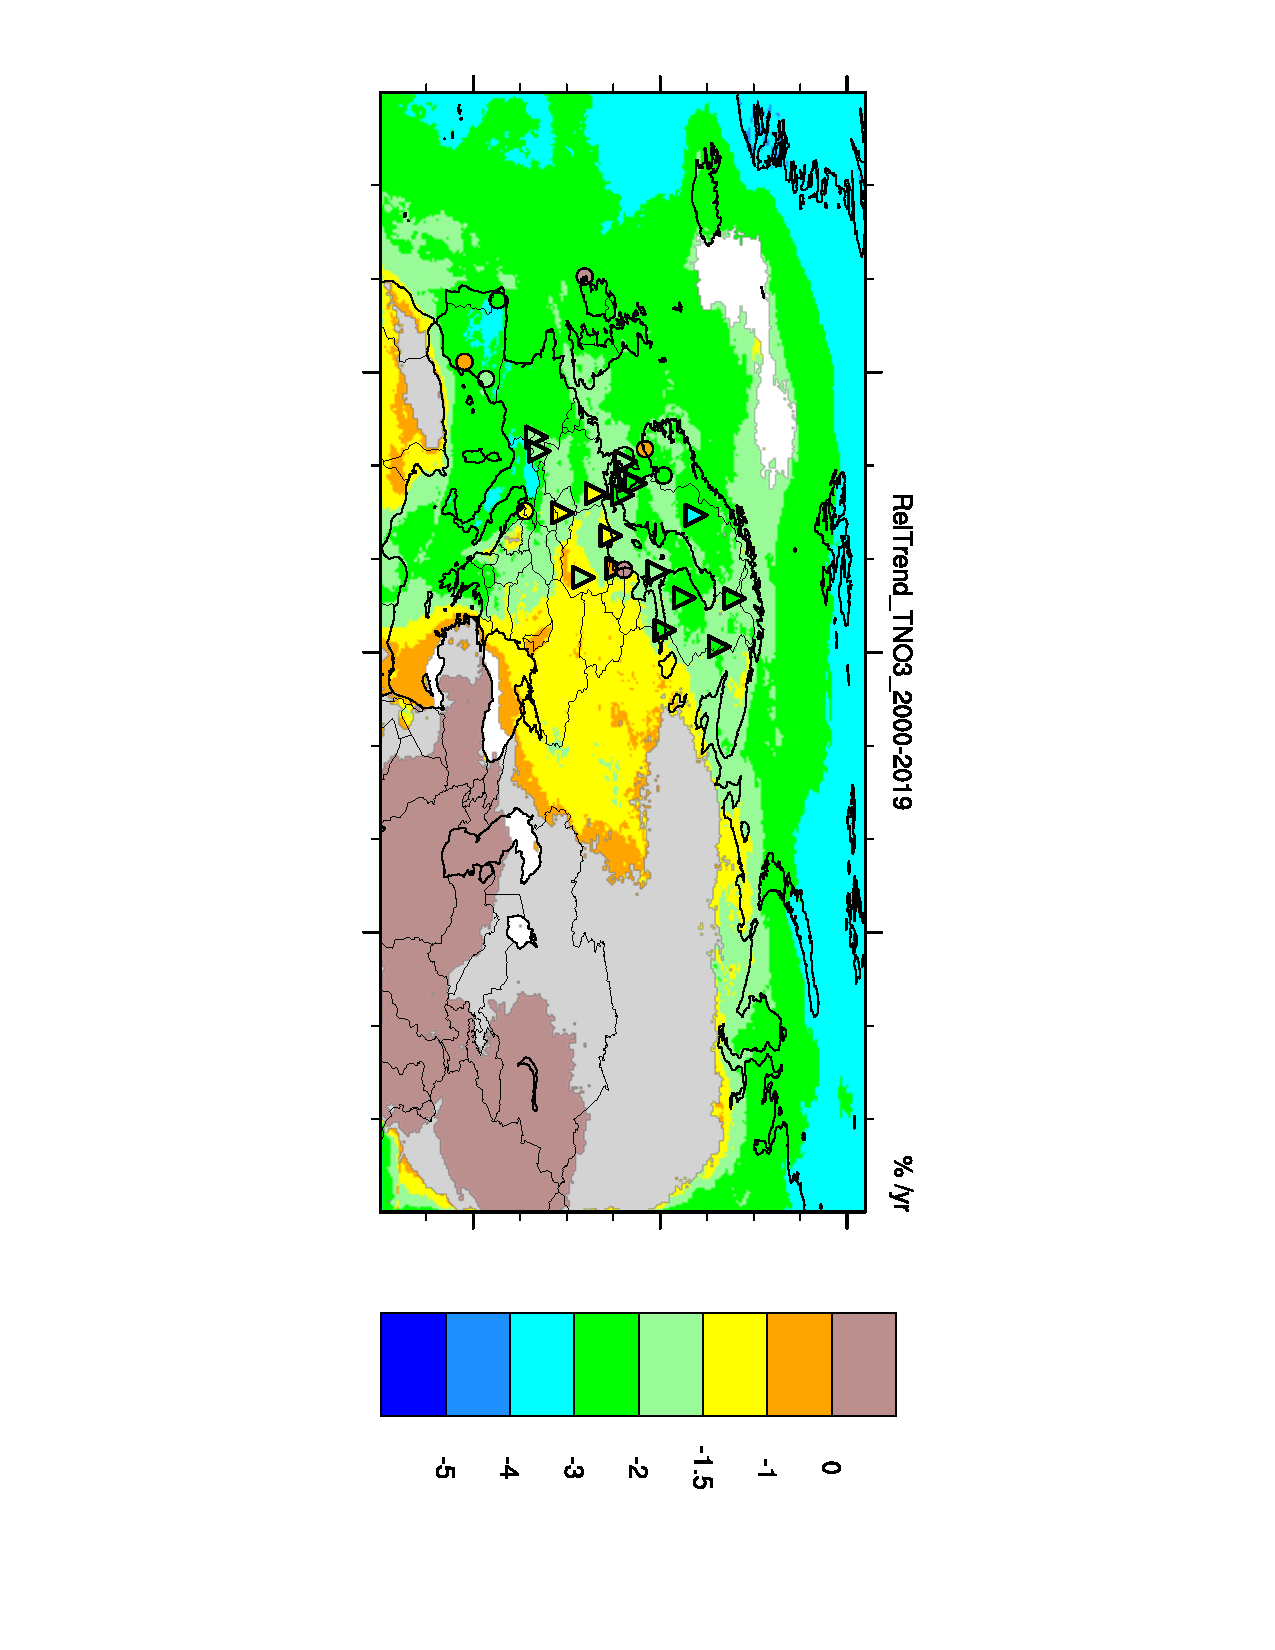
\includegraphics[clip=,angle=90,height=6.1cm,viewport=175 67 448 754]{FIGS_TRENDS/RelTrend_TNO3_2000-2019_Perc.pdf}}
\centering{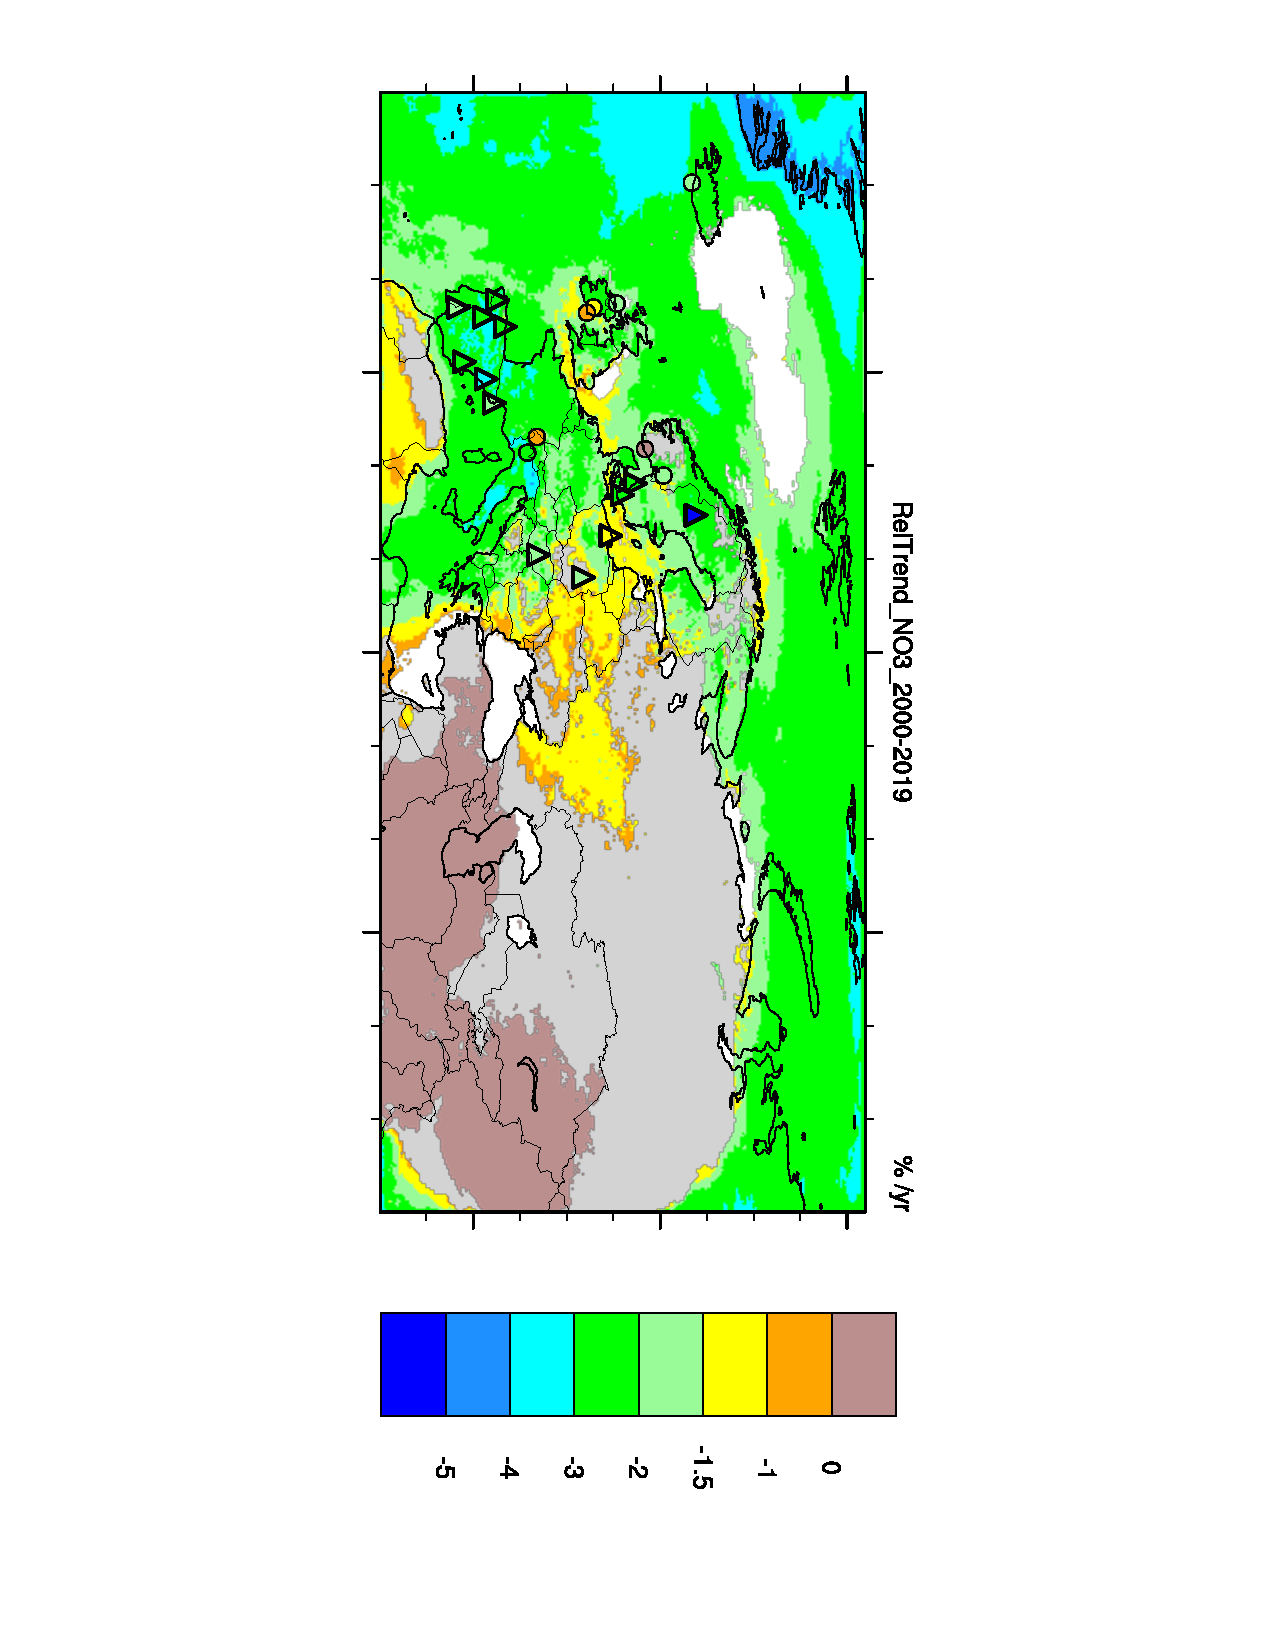
\includegraphics[clip=,angle=90,height=6.1cm,viewport=175 67 448 754]{FIGS_TRENDS/RelTrend_NO3_2000-2019_Perc.pdf}}
\centering{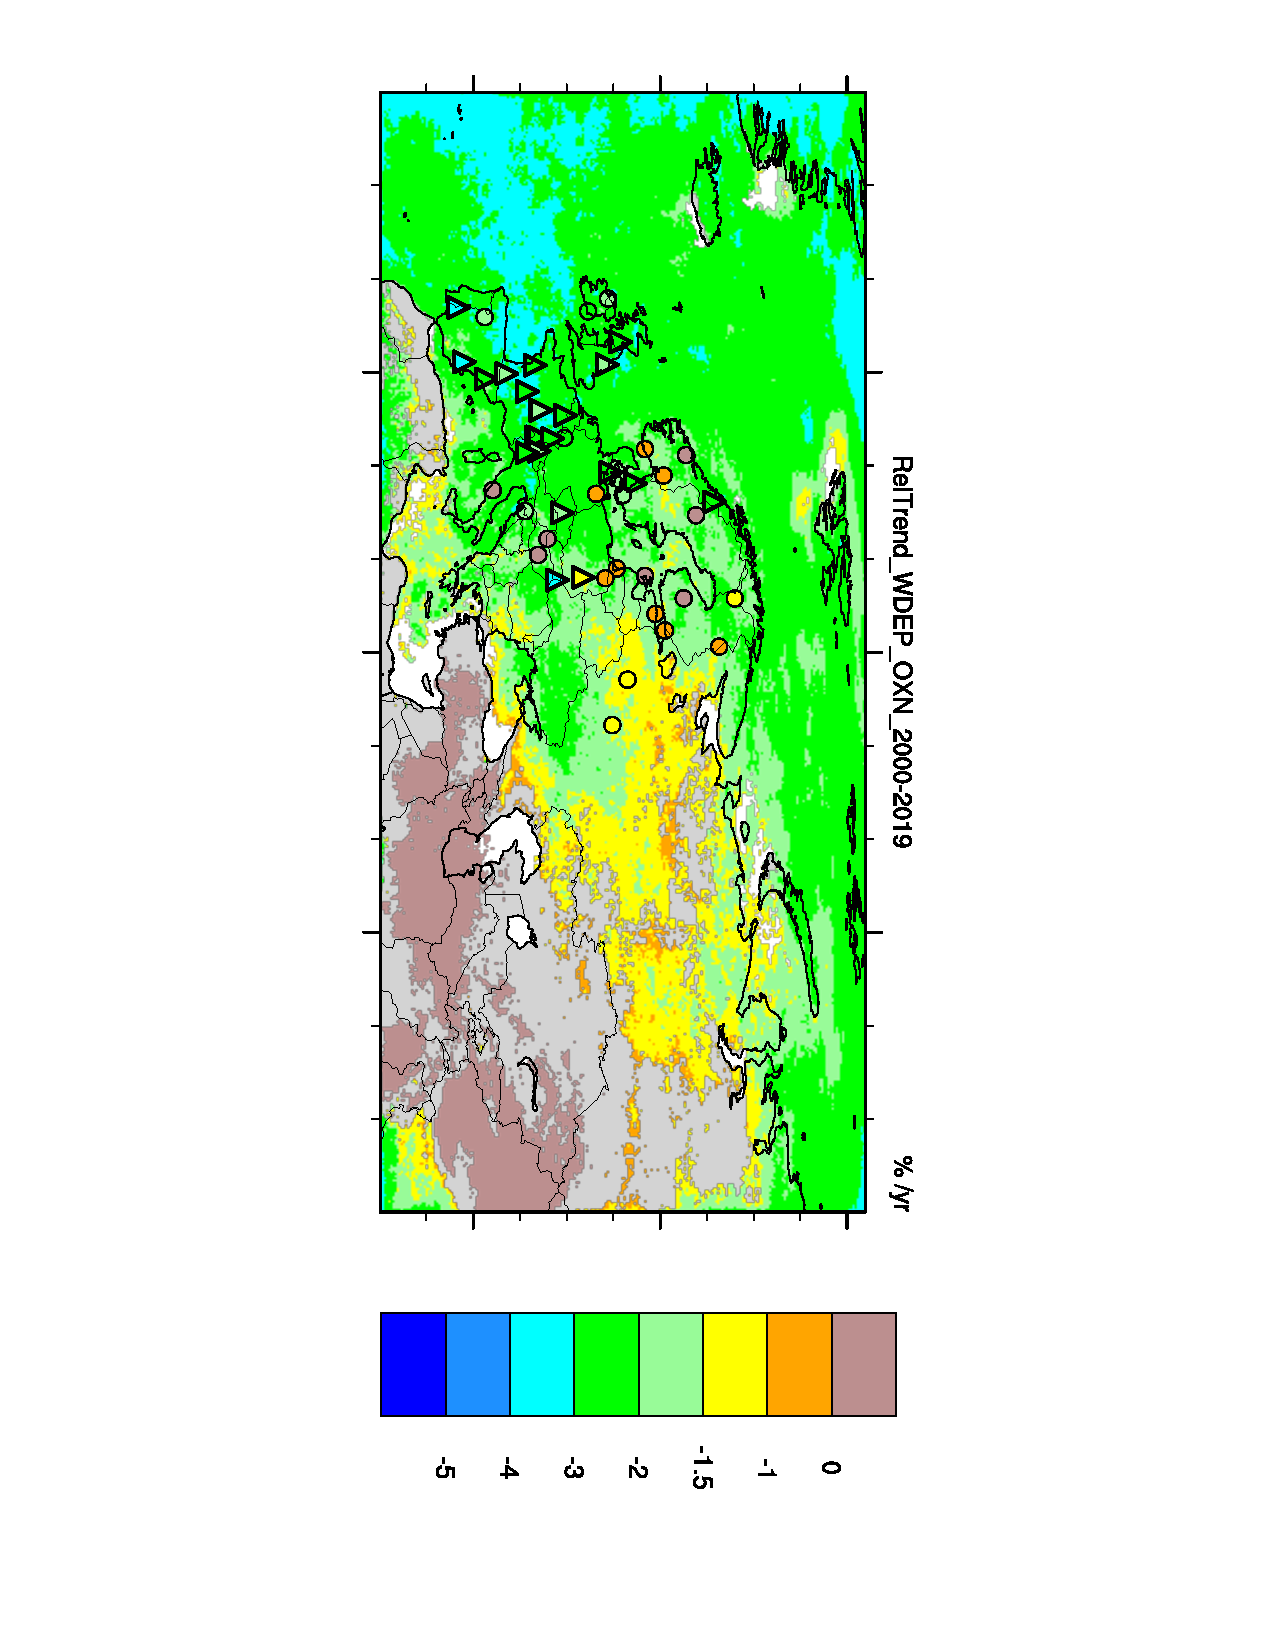
\includegraphics[clip=,angle=90,height=6.1cm,viewport=175 67 448 754]{FIGS_TRENDS/RelTrend_WDEP_OXN_2000-2019_Perc.pdf}}
\caption{Relative trends for NO$_2$, total nitrate, nitrate aerosol and wet deposition of oxidized nitrogen in the period of 2000-2019: EMEP modelled -- coloured contours (grey/white means non-significant trends) and
observed - coloured triangles (significant) and circles (non-significant).}
\label{fig:OXNtrends}
\end{figure}

\begin{table}[h]
\caption{\label{tab:no2_stat} Absolute and relative change and corresponding 95\% confidence intervals in observed and modelled annual and seasonal aggregated \noii concentrations for the different time periods. The number of sites with a significant outcome is provided}
\begin{center}
\scalebox{0.65}{%
\begin{tabular}{ll|ccc|cccc|cccc}
\toprule
          &        & \multicolumn{3}{c}{Number of sites} & \multicolumn{4}{c}{Average change (\ug $yr^{-1})$} & \multicolumn{4}{c}{Relative change (\% $yr^{-1}$)} \\
Period & Seasons &           total & sign.(obs.) & sign.(mod.) &                    obs. &          conf.interval &  mod. &          conf.interval &                     obs. &         conf.interval &  mod. &        conf.interval \\
\midrule
2000-2019 & all &              60 &          45 &          59 &                  -0.131 &    (-0.162, -0.1) & -0.191 &  (-0.235, -0.147) &                    -1.18 &  (-2.21, -0.15) & -2.25 &  (-2.42, -2.07) \\
          & winter &              61 &          30 &          58 &                  -0.151 &  (-0.192, -0.111) & -0.256 &  (-0.303, -0.209) &                    -1.13 &  (-2.03, -0.22) & -2.36 &  (-2.54, -2.19) \\
          & spring &              59 &          37 &          55 &                  -0.119 &   (-0.15, -0.088) & -0.158 &  (-0.201, -0.116) &                    -0.88 &   (-2.09, 0.32) & -2.07 &  (-2.26, -1.88) \\
          & summer &              59 &          39 &          55 &                  -0.092 &  (-0.118, -0.067) & -0.132 &   (-0.174, -0.09) &                    -1.18 &  (-2.07, -0.29) & -1.88 &  (-2.12, -1.64) \\
          & autumn &              59 &          41 &          58 &                  -0.149 &  (-0.186, -0.112) & -0.189 &  (-0.236, -0.141) &                    -1.13 &   (-2.41, 0.15) & -2.19 &  (-2.37, -2.01) \\
2005-2019 & all &              64 &          49 &          63 &                  -0.160 &  (-0.195, -0.125) & -0.194 &  (-0.237, -0.152) &                    -1.86 &  (-2.56, -1.16) & -2.58 &   (-2.8, -2.36) \\
2010-2019 & all &              66 &          36 &          52 &                  -0.184 &  (-0.226, -0.142) & -0.174 &  (-0.212, -0.135) &                    -2.65 &  (-3.39, -1.92) & -2.62 &  (-2.89, -2.35) \\
2000-2010 & all &              64 &          11 &          42 &                  -0.093 &  (-0.141, -0.044) & -0.181 &   (-0.231, -0.13) &                    -1.00 &  (-1.74, -0.27) & -1.98 &  (-2.36, -1.61) \\
\bottomrule
\end{tabular}}
\end{center}
\end{table}



\begin{table}[h]
\caption{\label{tab:tno3_stat} Absolute and relative change and corresponding 95\% confidence intervals in observed and modelled annual and seasonal aggregated concentrations of total nitrate ({\ensuremath{\mbox{HNO}_{\rm 3}}} + \noiii) in air and aerosols. The number of sites with a significant outcome is provided}
\begin{center}
\scalebox{0.65}{%
\begin{tabular}{ll|ccc|cccc|cccc}
\toprule
          &        & \multicolumn{3}{c}{Number of sites} & \multicolumn{4}{c}{Absolute change (\ug $yr^{-1})$} & \multicolumn{4}{c}{Relative change (\% $yr^{-1}$)} \\
Period & Seasons &           total & sign.(obs.) & sign.(mod.) &                    obs. &          conf.interval &  mod. &          conf.interval &                     obs. &         conf.interval &  mod. &        conf.interval \\
\midrule
2000-2019 & all &              25 &          17 &          25 &                  -0.008 &  (-0.011, -0.005) & -0.013 &   (-0.016, -0.01) &                    -1.60 &    (-2.0, -1.2) & -2.13 &  (-2.33, -1.94) \\
          & winter &              27 &           7 &          16 &                  -0.009 &  (-0.014, -0.003) & -0.014 &   (-0.018, -0.01) &                    -1.21 &  (-1.75, -0.66) & -1.93 &   (-2.26, -1.6) \\		  
          & spring &              25 &          13 &          21 &                  -0.010 &  (-0.013, -0.007) & -0.015 &  (-0.018, -0.011) &                    -1.69 &  (-2.08, -1.29) & -2.24 &  (-2.46, -2.02) \\
          & summer &              25 &          17 &          23 &                  -0.005 &  (-0.007, -0.003) & -0.012 &  (-0.015, -0.009) &                    -1.43 &   (-1.86, -1.0) & -2.27 &   (-2.43, -2.1) \\
          & autumn &              24 &          16 &          16 &                  -0.009 &  (-0.013, -0.006) & -0.014 &   (-0.019, -0.01) &                    -1.89 &  (-2.43, -1.35) & -2.20 &  (-2.48, -1.93) \\
2005-2019 & all &              31 &          18 &          26 &                  -0.011 &  (-0.014, -0.008) & -0.014 &  (-0.017, -0.011) &                    -2.29 &  (-2.74, -1.84) & -2.51 &   (-2.8, -2.22) \\
2010-2019 & all &              29 &          16 &           9 &                  -0.015 &   (-0.019, -0.01) & -0.010 &  (-0.014, -0.007) &                    -3.38 &   (-4.26, -2.5) & -2.16 &  (-2.58, -1.75) \\
2000-2010 & all &              33 &           7 &          11 &                  -0.006 &  (-0.011, -0.001) & -0.017 &  (-0.022, -0.012) &                    -0.54 &   (-1.55, 0.47) & -2.12 &  (-2.66, -1.57) \\
\bottomrule
\end{tabular}}
\end{center}
\end{table}

\begin{table}[h]
\caption{\label{tab:no3pm_stat}  Absolute and relative change and corresponding 95\% confidence intervals in observed and modelled annual and seasonal aggregated concentrations of  \noiii concentrations in aerosols. The number of sites with a significant outcome is provided}
\begin{center}
\scalebox{0.65}{%
\begin{tabular}{ll|ccc|cccc|cccc}
\toprule
          &        & \multicolumn{3}{c}{Number of sites} & \multicolumn{4}{c}{Absolute change (\ug $yr^{-1})$} & \multicolumn{4}{c}{Relative change (\% $yr^{-1}$)} \\
Period & Seasons &           total & sign.(obs.) & sign.(mod.) &                    obs. &          conf.interval &  mod. &          conf.interval &                     obs. &         conf.interval &  mod. &        conf.interval \\
\midrule
2000-2019 & all &              21 &          13 &          15 &                  -0.009 &  (-0.012, -0.006) & -0.014 &  (-0.018, -0.009) &                    -2.01 &  (-2.49, -1.53) & -2.53 &   (-2.86, -2.2) \\
          & winter &              20 &           8 &           5 &                  -0.012 &  (-0.018, -0.005) & -0.012 &  (-0.016, -0.008) &                    -1.85 &  (-2.77, -0.93) & -2.01 &  (-2.55, -1.47) \\
          & spring &              20 &          12 &          15 &                  -0.011 &  (-0.017, -0.005) & -0.012 &  (-0.018, -0.007) &                    -1.89 &  (-2.69, -1.09) & -2.21 &  (-2.97, -1.45) \\
          & summer &              20 &           8 &          13 &                  -0.004 &  (-0.006, -0.002) & -0.010 &  (-0.014, -0.006) &                    -1.55 &  (-2.17, -0.94) & -2.70 &  (-2.98, -2.43) \\
          & autumn &              20 &          11 &           9 &                  -0.010 &  (-0.013, -0.007) & -0.014 &  (-0.021, -0.007) &                    -2.41 &   (-2.8, -2.01) & -2.42 &  (-2.83, -2.01) \\
2005-2019 & all &              26 &          11 &          16 &                  -0.011 &  (-0.015, -0.006) & -0.014 &  (-0.018, -0.009) &                    -2.32 &  (-2.84, -1.81) & -2.77 &  (-3.21, -2.33) \\
2010-2019 & all &              32 &           3 &           6 &                  -0.010 &  (-0.015, -0.004) & -0.009 &  (-0.013, -0.005) &                    -1.98 &  (-2.85, -1.11) & -1.46 &  (-2.23, -0.68) \\
2000-2010 & all &              20 &           3 &           9 &                  -0.006 &   (-0.013, 0.001) & -0.020 &  (-0.028, -0.012) &                    -1.54 &   (-2.8, -0.27) & -3.01 &  (-3.99, -2.03) \\
\bottomrule
\end{tabular}}
\end{center}
\end{table}

\begin{table}[h]
\caption{\label{tab:hno3_stat} Absolute and relative change and corresponding 95\% confidence intervals in observed and modelled annual and seasonal aggregated concentrations of {\ensuremath{\mbox{HNO}_{\rm 3}}}. The number of sites with a significant outcome is provided.}
\begin{center}
\scalebox{0.65}{%
\begin{tabular}{ll|ccc|cccc|cccc}
\toprule
          &        & \multicolumn{3}{c}{Number of sites} & \multicolumn{4}{c}{Absolute change (\ug $yr^{-1})$} & \multicolumn{4}{c}{Relative change (\% $yr^{-1}$)} \\
Period & Seasons &           total & sign.(obs.) & sign.(mod.) &                    obs. &          conf.interval &  mod. &          conf.interval &                     obs. &         conf.interval &  mod. &        conf.interval \\
\midrule
2000-2019 & all &               6 &           4 &           6 &                  -0.002 &  (-0.004, -0.001) & -0.003 &  (-0.005, -0.002) &                    -1.94 &  (-2.77, -1.11) & -2.35 &  (-2.64, -2.07) \\
          & winter &               6 &           3 &           4 &                  -0.003 &  (-0.005, -0.001) & -0.002 &  (-0.003, -0.001) &                    -2.15 &  (-2.92, -1.37) & -2.80 &  (-3.71, -1.89) \\
          & spring &               6 &           4 &           6 &                  -0.002 &  (-0.004, -0.001) & -0.003 &  (-0.005, -0.002) &                    -2.05 &  (-3.15, -0.95) & -2.68 &  (-3.17, -2.19) \\
          & summer &               6 &           3 &           6 &                  -0.002 &  (-0.004, -0.001) & -0.004 &  (-0.006, -0.002) &                    -1.83 &   (-2.97, -0.7) & -1.85 &  (-2.06, -1.63) \\
          & autumn &               6 &           3 &           6 &                  -0.002 &    (-0.003, -0.0) & -0.003 &  (-0.004, -0.001) &                    -2.09 &  (-3.22, -0.97) & -2.49 &  (-2.99, -1.99) \\
2005-2019 & all &              12 &           7 &           9 &                  -0.004 &  (-0.005, -0.003) & -0.003 &  (-0.004, -0.001) &                    -2.48 &   (-3.16, -1.8) & -2.26 &  (-2.85, -1.67) \\
2010-2019 & all &              16 &           4 &           3 &                  -0.005 &  (-0.007, -0.003) & -0.002 &    (-0.003, -0.0) &                    -4.25 &  (-5.65, -2.86) & -0.67 &   (-2.31, 0.97) \\
2000-2010 & all &              10 &           3 &           4 &                  -0.006 &     (-0.012, 0.0) & -0.005 &  (-0.007, -0.003) &                    -1.63 &   (-3.86, 0.61) & -3.33 &   (-4.17, -2.5) \\
\bottomrule
\end{tabular}}
\end{center}
\end{table}


\begin{table}[h]
\caption{\label{tab:no3dep_stat}Absolute and relative change and corresponding 95\% confidence intervals in observed and modelled annual and seasonal aggregated wet deposition of nitrate for the different time periods. The number of sites with a significant outcome is provided.}
\begin{center}
\scalebox{0.7}{%
\begin{tabular}{ll|ccc|cccc|cccc}
\toprule
          &        & \multicolumn{3}{c}{Number of sites} & \multicolumn{4}{c}{Absolute change (\ugN $m^{2} yr^{-1}$)} & \multicolumn{4}{c}{Relative change (\% $yr^{-1}$)} \\
Period & Seasons &           total & sign.(obs.) & sign.(mod.) &                    obs. &          conf.interval &  mod. &          conf.interval &                     obs. &         conf.interval &  mod. &        conf.interval \\
\midrule
2000-2019 & all &              46 &          21 &          44 &                   -12.1 &   (-15.7, -8.5) & -26.4 &  (-31.3, -21.4) &                    -1.36 &    (-1.74, -0.98) & -2.35 &  (-2.49, -2.21) \\
          & winter &              45 &           6 &          25 &                    -8.3 &   (-12.4, -4.3) & -19.9 &  (-23.5, -16.4) &                    -1.16 &    (-1.69, -0.63) & -2.23 &   (-2.46, -2.0) \\
          & spring &              43 &          17 &          33 &                   -14.2 &   (-20.5, -7.9) & -27.8 &  (-35.2, -20.3) &                    -1.11 &    (-1.74, -0.48) & -2.33 &  (-2.54, -2.12) \\
          & summer &              45 &          10 &          33 &                   -11.3 &   (-16.3, -6.2) & -30.4 &  (-37.4, -23.3) &                    -0.02 &     (-1.83, 1.78) & -2.17 &   (-2.44, -1.9) \\
          & autumn &              45 &          12 &          28 &                   -12.8 &   (-16.6, -9.0) & -25.6 &  (-31.6, -19.7) &                    -1.53 &    (-2.01, -1.05) & -2.36 &  (-2.59, -2.13) \\
2005-2019 & all &              50 &          15 &          40 &                   -10.0 &   (-14.8, -5.2) & -24.0 &  (-27.7, -20.3) &                    -0.53 &     (-2.04, 0.98) & -2.62 &   (-2.8, -2.44) \\
2010-2019 & all &              58 &           7 &          19 &                   -13.3 &   (-17.6, -8.9) & -23.6 &  (-28.3, -18.9) &                    -1.54 &    (-2.23, -0.86) & -2.60 &  (-2.98, -2.22) \\
2000-2010 & all &              45 &           8 &          15 &                   -13.2 &   (-20.8, -5.5) & -26.4 &  (-34.3, -18.5) &                    -1.12 &    (-2.22, -0.03) & -2.24 &  (-2.65, -1.83) \\
\bottomrule
\end{tabular}}
\end{center}
\end{table}



\section{\label{sec:Trends_reduced nitrogen }Trends in reduced nitrogen}
Ammonia emissions from agricultural activities have been only slightly reduced for the western EMEP domain since 2000 (-12\% in EU27+UK+EFTA countries). In the EMEP domain as a whole, ammonia emissions have increased by 12\% since 2000 (see chapter \ref{ch:emis2019}).

With such small changes in emissions, clearly it is very difficult to detect any trends in the observations - considering also that the meteorological variability introduces year to year changes of the same magnitude as the expected trends.
Note that previous studies (e.g. \cite{torseth2012} and \cite{Theobald2019}) have found decreasing trends for reduced nitrogen. However, those studies analyzed earlier periods (e.g. 1980-2009 or 1990-2009), where the reported ammonia emissions decreased more.

Figure~\ref{fig:Nred_trends} shows an overview of the annual and seasonal trends in reduced nitrogen compounds from 2000 to 2019. Figure~\ref{fig:RDNtrends} visualizes the trends in different reduced nitrogen compounds from observations on top of modelled trends on a European map. Tables~\ref{tab:tnh4_stat} to \ref{tab:nh4dep_stat} show absolute and relative changes in the different reduced nitrogen compounds.

Indeed, both observations and model calculations find very few significant trends in wet deposition of reduced nitrogen. Out of 47 sites with long term measurements at EMEP background sites, only 14 (8) are significant for the observations (model). The average change in the observations for 2000 to 2019 is -0.14\% yr$^{-1}$, with a confidence interval from -0.1\% yr$^{-1}$ to +0.52\% yr$^{-1}$, while the model show an average trend of -0.4\% yr$^{-1}$ and a confidence interval of -0.7\% yr$^{-1}$ to -0.1\% yr$^{-1}$. For the shorter time periods (2000-2010 and 2010-2019) there are even fewer sites with significant trends (see Table~\ref{tab:nh4dep_stat}).

Total ammonium (NH$_3$ + NH$_4$) in air show larger negative changes in observations (model) of about -1.45\% yr$^{-1}$ (-1.33\% yr$^{-1}$) and with a larger fraction of the sites having significant trends. This trend is larger than the reduction in ammonia emissions for EU27+UK+EFTA countries (-12\%), in total 27\% (25\%) in observations (model calculations) for 2000-2019.

The trend for ammonium aerosols is even more negative, -2.61 and -2.51 \% yr$^{-1}$ in observations and model calculations, respectively.

Very few sites have long term time series of ammonia in air (8 sites), and very few of the trends calculated are significant. However, on average, the changes observed and calculated are positive: +1.55 and +1.28 \% yr$^{-1}$ in observations and model calculations, respectively, with all values within the confidence interval being positive.

This large difference between the trends of the different reduced nitrogen components can be explained by the interaction of ammonia with the sulphur and nitrogen components. When ammonia is released into the air, it reacts with secondary sulphate originating from the SO$_x$ emissions and forms particulate ammonium sulphates. If more ammonia is available, it reacts with nitric acid in an equilibrium reaction to form particulate ammonium nitrate. During the years from 2000 onwards, large reductions in SO$_x$ and NO$_x$ emissions have taken place, and thus less sulphate and nitric acid is available for forming ammonium particles. Therefore, a smaller fraction of NH$_3$ is converted to aerosol ammonium, and the decrease in particulate ammonium is strongly linked to the decrease in sulphate and nitrate. It is therefore to be expected that the trend in ammonium aerosol (-2.6\% yr$^{-1}$, observations) lies somewhere between the trend in particulate sulphate (-3.21\% yr$^{-1}$, observations) and nitrate (-2.01\% yr$^{-1}$, observations). 

When less ammonia is converted to ammonium, the (very small) decrease in ammonia emissions is compensated by a larger part of ammonia residing in gas phase, and no decrease in ammonia (very few significant trends) are detected.

For the sum of ammonia and ammonium, the two opposite trends of ammonia (no trend or slighly positive) and ammonium (negative) results in a negative trend that is smaller than the trend for ammonium alone.

The analysis done for the shorter time periods (2000-2010 and 2010-2019) confirms the findings discussed above. It is worth to note that the agreement between the trends calculated from model calculations and the observation are excellent for the different reduced nitrogen components, which indicates that the EMEP MSC-W model does a very good job in reproducing the non-linear interactions between sulphur, oxidized nitrogen and reduced nitrogen and how it has evolved during the past 20 years.

In summary, the observations and the model calculations confirm that very small reductions of ammonia emissions have been achieved during the 2000-2019 period. However, the contribution of ammonia emission to aerosols have been largely reduced during this period, due to the impact of SO$_x$ and NO$_x$ emission reductions.





\begin{figure}
	\centering
	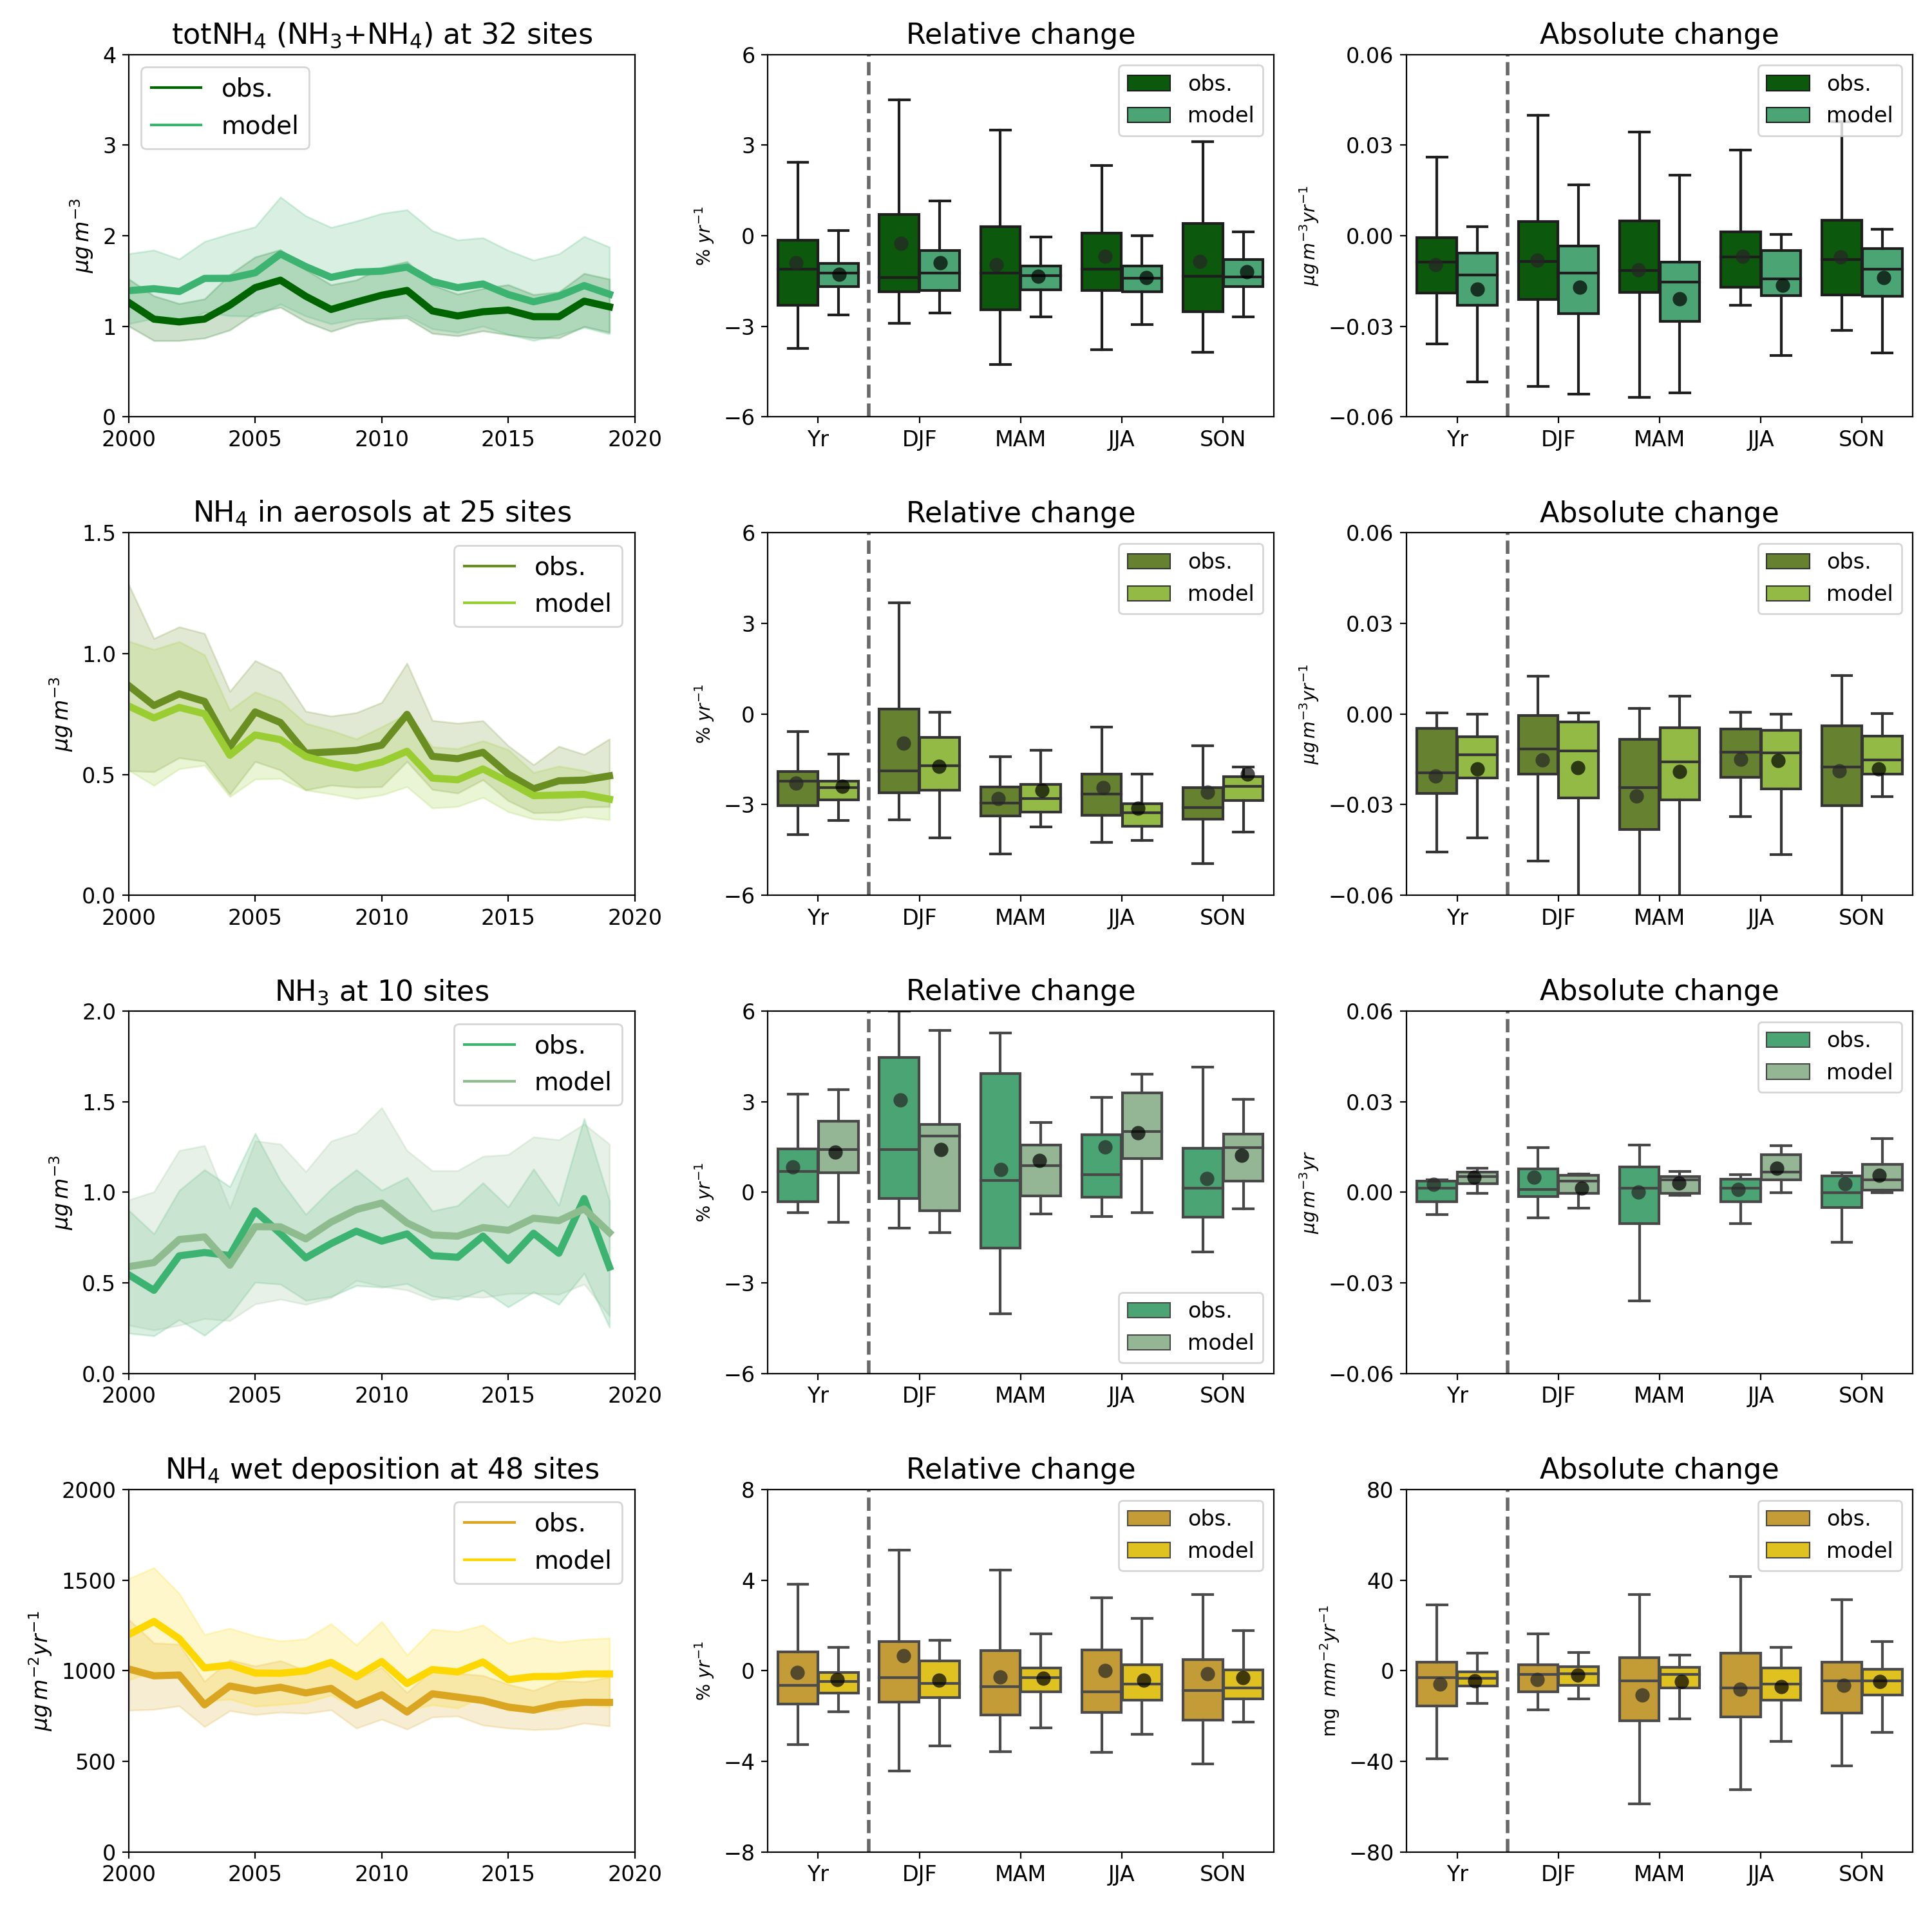
\includegraphics[width=0.74\paperwidth]{FIGS_TRENDS/Nred_trends.png}
	\caption{\label{fig:Nred_trends}Trends in oxidised nitrogen components from 2010-2019 for EMEP observations and model.The solid line in the trend plots indicate the average annual mean concentrations for all the sites and the shaded area the 95 \% confidence interval. The box plot represent the 50,25,75 percentiles and the whiskers lie within the 1.5 inter-quartile ranges for the trends of all the sites, including those with not significant trends. In addition, the mean trends are indicated with black circles and the trend in \nhiii emission is indicated in the plot of total ammonium with secondary y-axes}
\end{figure}

\begin{figure}[h]
  \centering{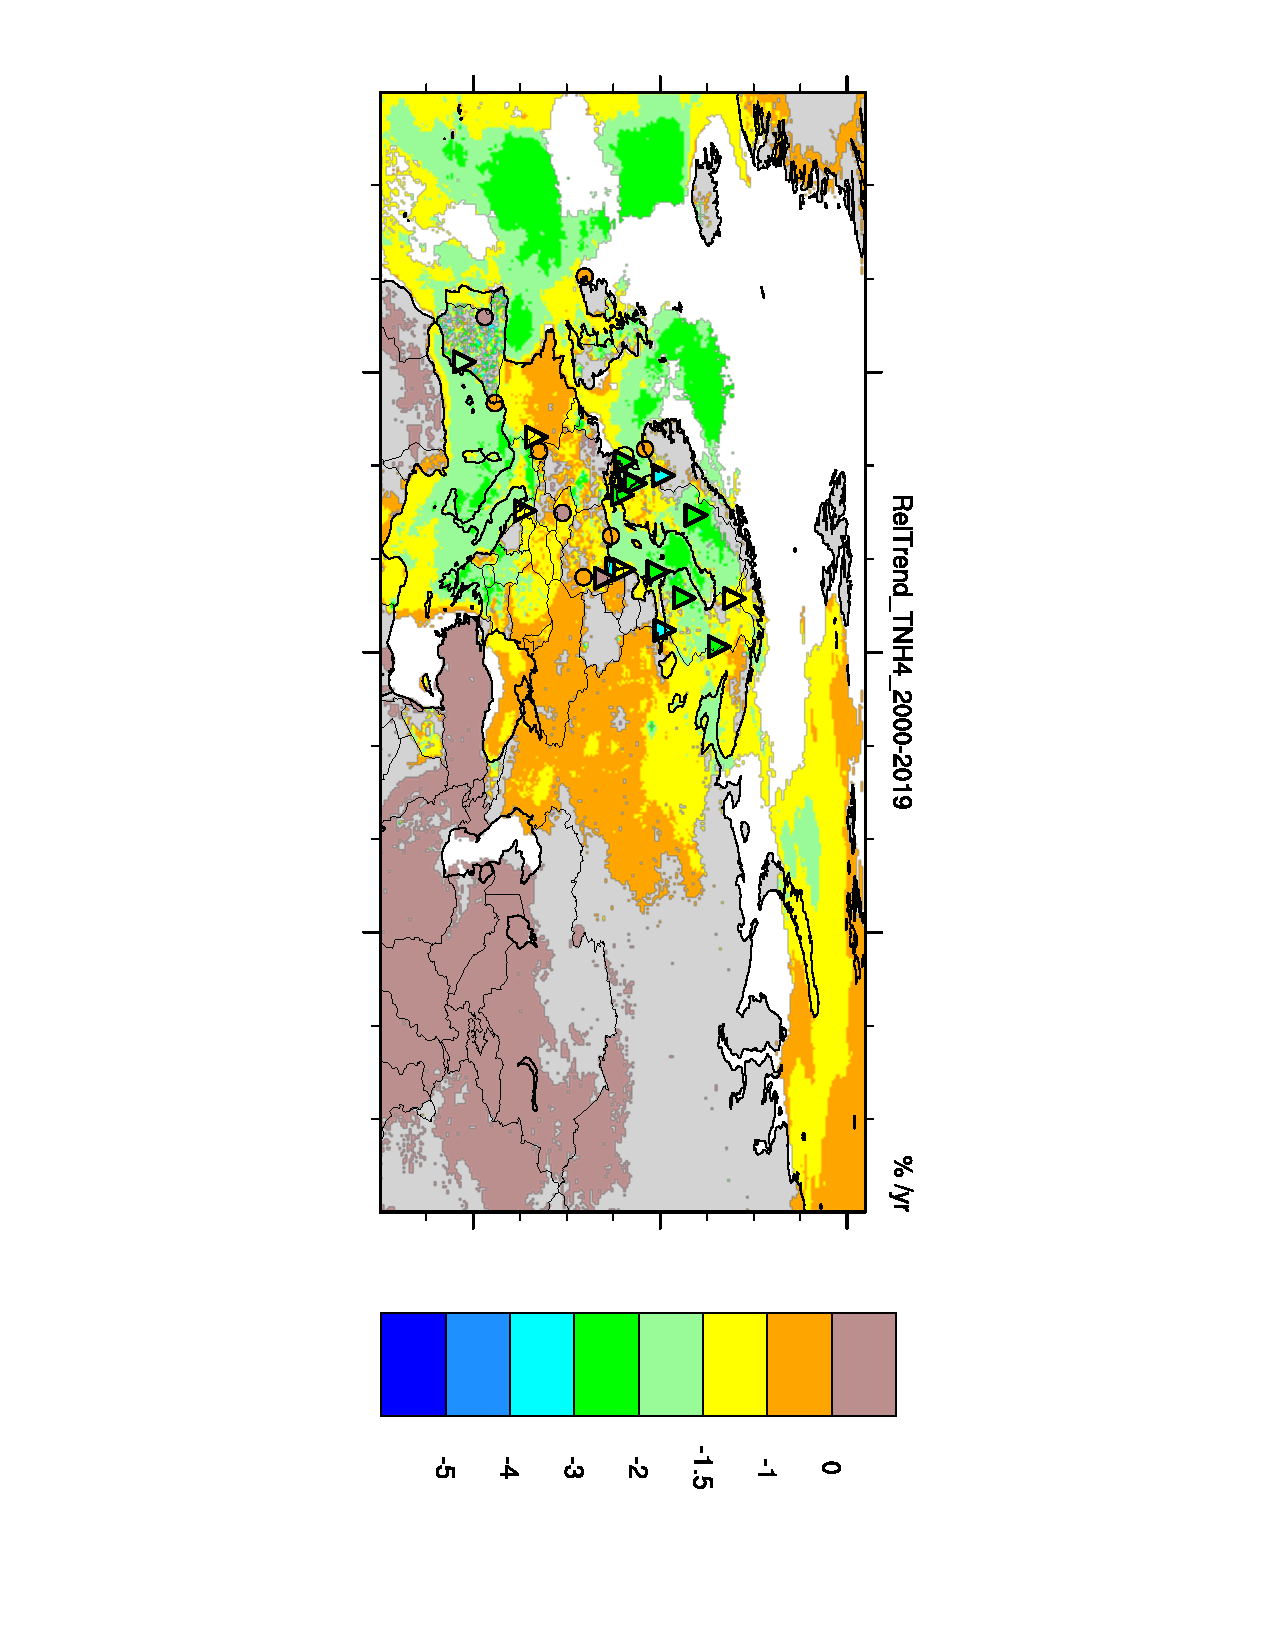
\includegraphics[clip=,angle=90,height=6.1cm,viewport=175 67 448 754]{FIGS_TRENDS/RelTrend_TNH4_2000-2019_Perc.pdf}}
%  \vspace{0.5cm}
  \centering{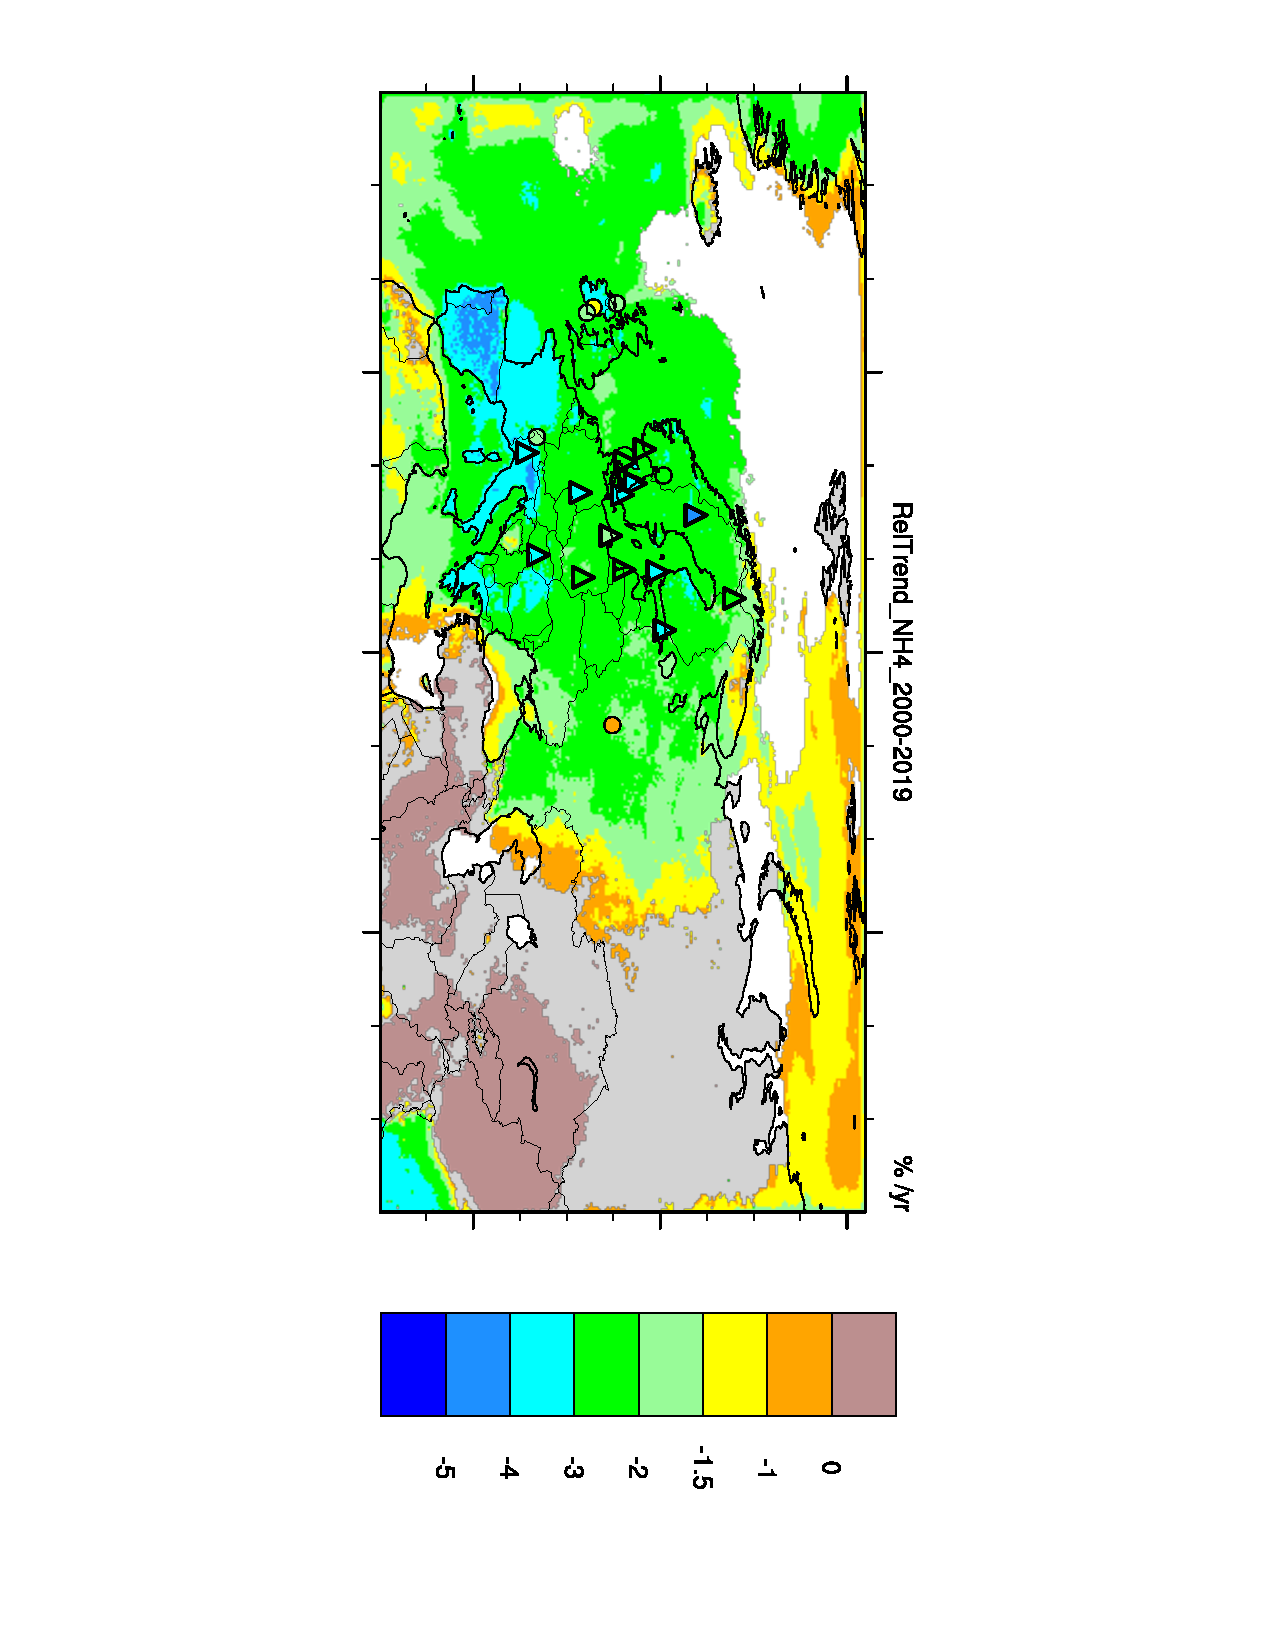
\includegraphics[clip=,angle=90,height=6.1cm,viewport=175 67 448 754]{FIGS_TRENDS/RelTrend_NH4_2000-2019_Perc.pdf}}
\centering{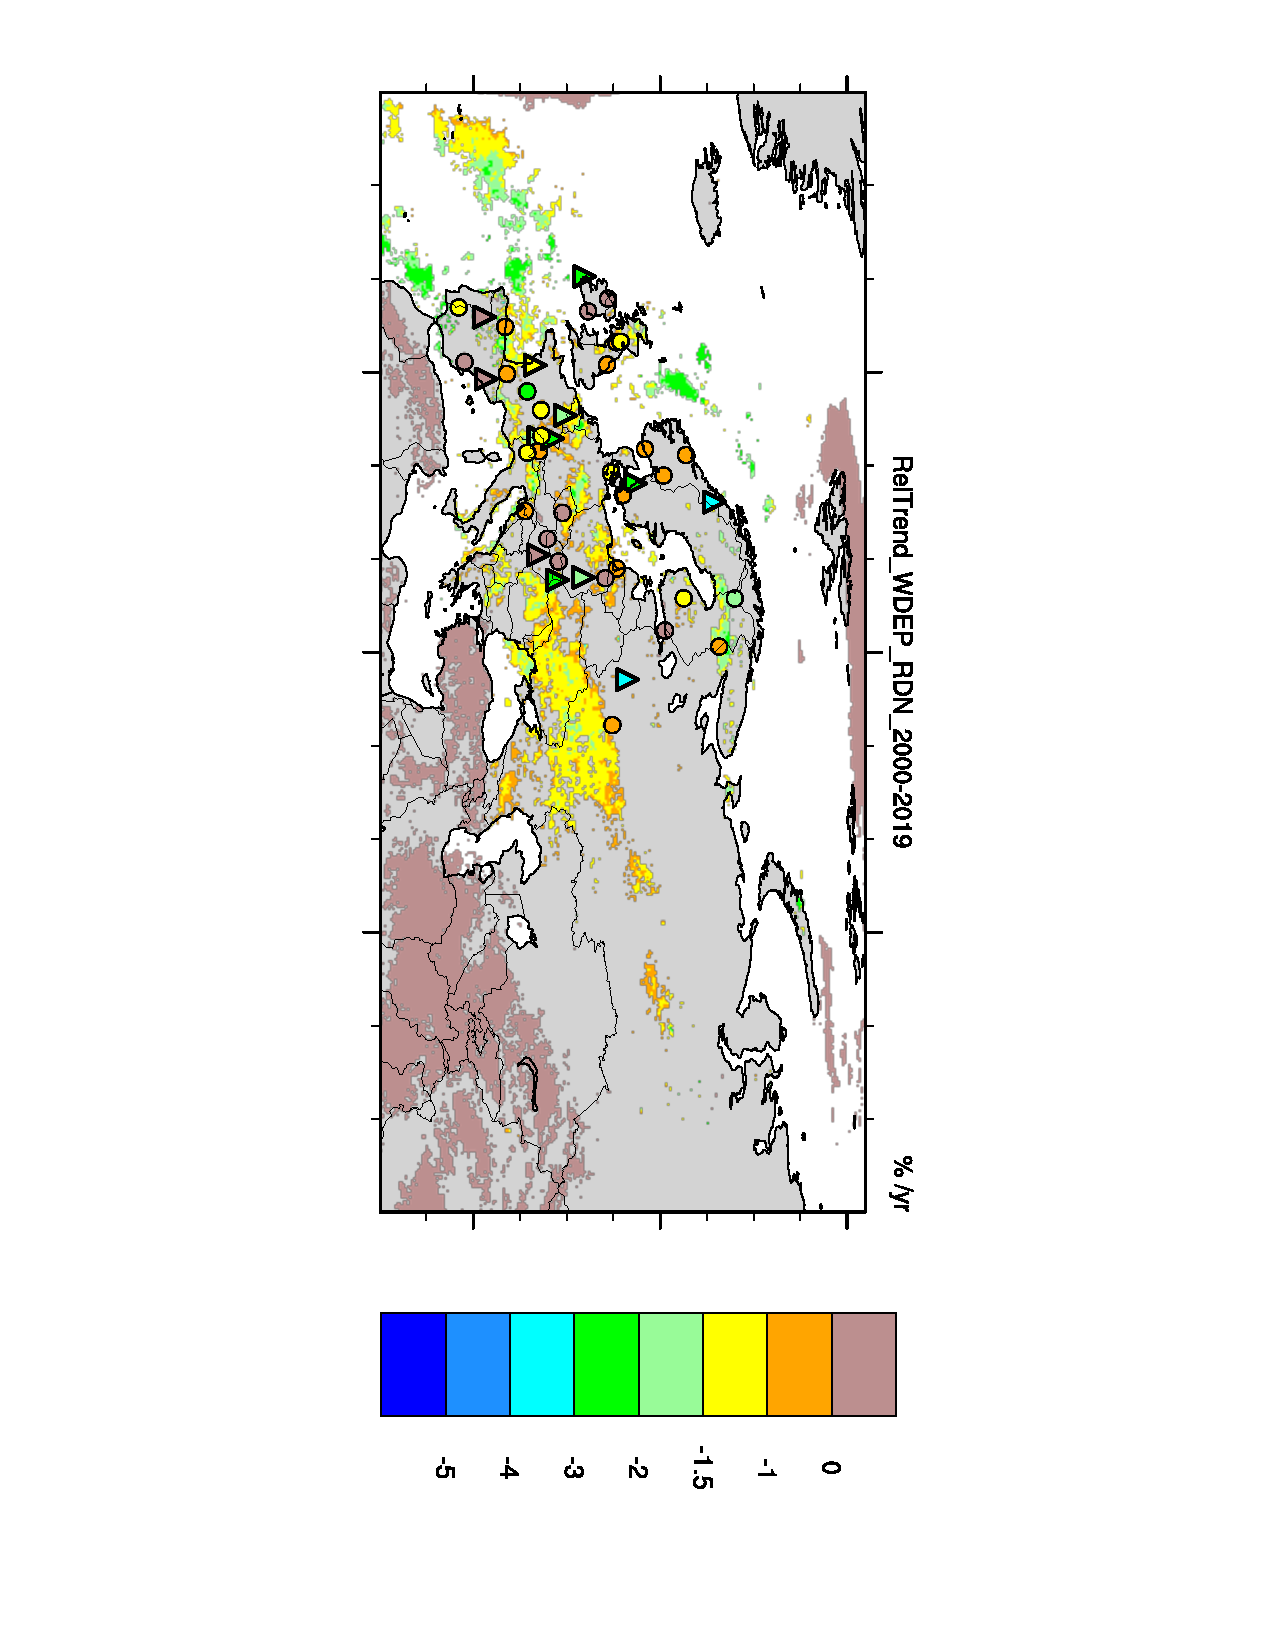
\includegraphics[clip=,angle=90,height=6.1cm,viewport=175 67 448 754]{FIGS_TRENDS/RelTrend_WDEP_RDN_2000-2019_Perc.pdf}}
\caption{Relative trends for total ammonium (sum of ammonia and aerosol ammonium), aerosol ammonium and wet deposition of reduced nitrogen in the period of 2000-2019: EMEP modelled -- coloured contours (grey/white means non-significant trends) and
observed - coloured triangles (significant) and circles (non-significant).}
\label{fig:RDNtrends}
\end{figure}

\begin{table}
\caption{\label{tab:tnh4_stat} Absolute and relative change and corresponding 95\% confidence intervals in observed and modelled annual and seasonal aggregated concentrations of total ammonium (\nhiii+\nhiv) in air and aerosols for the different time periods. The number of sites with a significant outcome is provided.}
\begin{center}
\scalebox{0.65}{%
\begin{tabular}{ll|ccc|cccc|cccc}
\toprule
          &        & \multicolumn{3}{c}{Number of sites} & \multicolumn{4}{c}{Absolute change (\ug $yr^{-1})$} & \multicolumn{4}{c}{Relative change (\% $yr^{-1}$)} \\
Period & Seasons &           total & sign.(obs.) & sign.(mod.) &                    obs. &          conf.interval &  mod. &          conf.interval &                     obs. &         conf.interval &  mod. &        conf.interval \\
\midrule
2000-2019 & all &              25 &          17 &          18 &                  -0.016 &  (-0.024, -0.007) & -0.019 &  (-0.027, -0.012) &                    -1.45 &  (-1.99, -0.91) & -1.36 &  (-1.58, -1.14) \\
          & winter &              28 &           9 &          10 &                  -0.018 &  (-0.029, -0.008) & -0.023 &  (-0.033, -0.013) &                    -1.18 &  (-1.72, -0.64) & -1.14 &  (-1.47, -0.81) \\
          & spring &              25 &          10 &          16 &                  -0.017 &  (-0.029, -0.006) & -0.023 &  (-0.032, -0.015) &                    -1.48 &  (-2.21, -0.75) & -1.46 &   (-1.71, -1.2) \\
          & summer &              25 &          10 &          20 &                  -0.009 &  (-0.018, -0.001) & -0.017 &  (-0.025, -0.009) &                    -1.02 &  (-1.61, -0.44) & -1.44 &  (-1.71, -1.18) \\
          & autumn &              24 &          11 &           7 &                  -0.015 &  (-0.025, -0.006) & -0.016 &  (-0.023, -0.009) &                    -1.67 &  (-2.27, -1.08) & -1.32 &  (-1.61, -1.03) \\
2005-2019 & all &              27 &          12 &          12 &                  -0.019 &  (-0.029, -0.009) & -0.020 &  (-0.029, -0.011) &                    -1.90 &  (-2.55, -1.24) & -1.53 &  (-1.88, -1.18) \\
2010-2019 & all &              27 &           6 &           7 &                  -0.017 &  (-0.026, -0.008) & -0.012 &  (-0.021, -0.004) &                    -2.31 &  (-3.25, -1.36) & -1.12 &   (-1.75, -0.5) \\
2000-2010 & all &              37 &           6 &          13 &                  -0.022 &   (-0.034, -0.01) & -0.024 &  (-0.033, -0.016) &                    -1.36 &  (-2.11, -0.62) & -1.20 &  (-1.82, -0.58) \\
\bottomrule
\end{tabular}}
\end{center}
\end{table}

\begin{table}
\caption{\label{tab:nh4pm_stat} Absolute and relative change and corresponding 95\% confidence intervals in observed and modelled annual and seasonal aggregated concentrations of \nhiv in aerosols for the different time periods.The number of sites with a significant outcome is provided.}
\begin{center}
\scalebox{0.65}{%
\begin{tabular}{ll|ccc|cccc|cccc}
\toprule
          &        & \multicolumn{3}{c}{Number of sites} & \multicolumn{4}{c}{Absolute change (\ug $yr^{-1})$} & \multicolumn{4}{c}{Relative change (\% $yr^{-1}$)} \\
Period & Seasons &           total & sign.(obs.) & sign.(mod.) &                    obs. &          conf.interval &  mod. &          conf.interval &                     obs. &         conf.interval &  mod. &        conf.interval \\
\midrule
2000-2019 & all &              21 &          15 &          20 &                  -0.024 &  (-0.033, -0.016) & -0.021 &  (-0.028, -0.014) &                    -2.61 &  (-3.01, -2.22) & -2.61 &  (-2.79, -2.43) \\
          & winter &              22 &          10 &           9 &                  -0.019 &  (-0.035, -0.002) & -0.020 &  (-0.028, -0.013) &                    -1.47 &  (-2.49, -0.45) & -1.94 &  (-2.43, -1.45) \\
          & spring &              20 &          17 &          16 &                  -0.032 &  (-0.043, -0.021) & -0.022 &   (-0.03, -0.015) &                    -3.09 &  (-3.64, -2.55) & -2.74 &  (-3.17, -2.31) \\
          & summer &              20 &          14 &          20 &                  -0.017 &  (-0.023, -0.012) & -0.018 &  (-0.023, -0.013) &                    -2.78 &  (-3.22, -2.35) & -3.39 &  (-3.62, -3.16) \\
          & autumn &              19 &          11 &          11 &                  -0.023 &  (-0.031, -0.014) & -0.022 &  (-0.032, -0.012) &                    -2.75 &  (-3.65, -1.85) & -2.58 &   (-2.8, -2.35) \\
2005-2019 & all &              27 &          16 &          23 &                  -0.025 &  (-0.033, -0.017) & -0.022 &  (-0.028, -0.016) &                    -2.90 &  (-3.41, -2.38) & -3.01 &   (-3.2, -2.83) \\
2010-2019 & all &              31 &          16 &          17 &                  -0.029 &  (-0.041, -0.017) & -0.019 &  (-0.027, -0.012) &                    -3.48 &   (-4.7, -2.26) & -3.22 &   (-3.9, -2.54) \\
2000-2010 & all &              23 &           9 &          12 &                  -0.034 &   (-0.048, -0.02) & -0.036 &  (-0.047, -0.024) &                    -3.43 &   (-4.6, -2.27) & -3.18 &  (-3.63, -2.73) \\
\bottomrule
\end{tabular}}
\end{center}
\end{table}

\begin{table}
\caption{\label{tab:nh3_stat} Absolute and relative change and corresponding 95\% confidence intervals in observed and modelled annual and seasonal aggregated concentrations of \nhiii for the different time periods. The number of sites with a significant outcome is provided.}
\begin{center}
\scalebox{0.65}{%
\begin{tabular}{ll|ccc|cccc|cccc}
\toprule
          &        & \multicolumn{3}{c}{Number of sites} & \multicolumn{4}{c}{Absolute change (\ug $yr^{-1})$} & \multicolumn{4}{c}{Relative change (\% $yr^{-1}$)} \\
Period & Seasons &           total & sign.(obs.) & sign.(mod.) &                    obs. &          conf.interval &  mod. &          conf.interval &                     obs. &         conf.interval &  mod. &        conf.interval \\
\midrule
2000-2019 & all &               8 &           2 &           6 &                   0.010 &  (-0.005, 0.024) &  0.006 &  (-0.006, 0.017) &                     1.55 &    (0.22, 2.88) &  1.54 &   (0.42, 2.66) \\
          & winter &               8 &           1 &           3 &                   0.007 &  (-0.001, 0.016) &  0.002 &  (-0.007, 0.011) &                     4.03 &    (0.61, 7.44) &  1.47 &    (0.1, 2.84) \\
          & spring &               8 &           3 &           3 &                   0.011 &   (-0.007, 0.03) &  0.003 &  (-0.005, 0.011) &                     1.76 &   (-0.32, 3.83) &  1.46 &   (0.09, 2.84) \\
          & summer &               8 &           1 &           6 &                   0.013 &  (-0.009, 0.035) &  0.009 &   (-0.002, 0.02) &                     2.53 &    (-0.3, 5.36) &  2.27 &   (0.88, 3.65) \\
          & autumn &               8 &           1 &           4 &                   0.008 &   (-0.005, 0.02) &  0.007 &  (-0.001, 0.015) &                     0.94 &   (-0.36, 2.24) &  1.49 &   (0.65, 2.33) \\
2005-2019 & all &              18 &           3 &           7 &                   0.005 &  (-0.002, 0.012) &  0.000 &   (-0.009, 0.01) &                     0.57 &   (-0.26, 1.39) &  0.84 &    (0.1, 1.59) \\
2010-2019 & all &              22 &           4 &           5 &                   0.012 &  (-0.009, 0.032) &  0.001 &  (-0.017, 0.019) &                     2.80 &   (-1.35, 6.95) &  2.58 &   (0.67, 4.49) \\
2000-2010 & all &              12 &           3 &           4 &                   0.003 &  (-0.021, 0.028) &  0.012 &     (0.0, 0.025) &                     3.14 &     (0.5, 5.78) &  1.99 &    (0.4, 3.57) \\
\bottomrule
\end{tabular}}
\end{center}
\end{table}

\begin{table}
\caption{\label{tab:nh4dep_stat} Absolute and relative change and corresponding 95\% confidence intervals in observed and modelled annual and seasonal aggregated data of wet deposition of ammonium for the different time periods. The number of sites with a significant outcome is provided.}
\begin{center}
\scalebox{0.7}{%
\begin{tabular}{ll|ccc|cccc|cccc}
\toprule
          &        & \multicolumn{3}{c}{Number of sites} & \multicolumn{4}{c}{Average change (\ugN $m^{2} yr^{-1}$)} & \multicolumn{4}{c}{Relative change (\% $yr^{-1}$)} \\
Period & Seasons &           total & sign.(obs.) & sign.(mod.) &                    obs. &          conf.interval &  mod. &          conf.interval &                     obs. &         conf.interval &  mod. &        conf.interval \\
\midrule
2000-2019 & all &              44 &          13 &           9 &                    -7.4 &  (-11.8, -3.0) &  -4.8 &   (-8.1, -1.5) &                    -0.31 &   (-0.99, 0.37) & -0.40 &  (-0.71, -0.09) \\
          & winter &              44 &           5 &           3 &                    -5.3 &   (-9.4, -1.3) &  -1.7 &    (-3.8, 0.4) &                    -0.25 &   (-0.94, 0.43) & -0.39 &  (-0.72, -0.06) \\
          & spring &              42 &           5 &           4 &                   -12.2 &  (-19.4, -4.9) &  -4.7 &   (-11.5, 2.1) &                    -0.39 &    (-1.1, 0.31) & -0.27 &   (-0.64, 0.11) \\
          & summer &              43 &           9 &           6 &                   -10.4 &  (-16.7, -4.1) &  -8.0 &  (-11.6, -4.4) &                    -0.12 &   (-1.17, 0.93) & -0.48 &  (-0.84, -0.12) \\
          & autumn &              43 &          10 &           4 &                    -7.5 &  (-12.8, -2.3) &  -5.2 &   (-9.3, -1.0) &                    -0.45 &   (-1.37, 0.47) & -0.35 &    (-0.8, 0.11) \\
2005-2019 & all &              52 &           8 &           4 &                    -4.8 &   (-10.7, 1.0) &  -3.4 &   (-6.4, -0.3) &                    -0.12 &   (-0.95, 0.71) & -0.43 &  (-0.78, -0.08) \\
2010-2019 & all &              62 &           3 &           4 &                    -2.7 &    (-8.6, 3.1) &  -5.8 &  (-11.1, -0.4) &                     0.90 &   (-0.95, 2.75) & -0.47 &   (-1.04, 0.11) \\
2000-2010 & all &              44 &           4 &           3 &                    -9.3 &  (-17.8, -0.8) &  -4.0 &   (-12.2, 4.2) &                    -0.36 &   (-1.24, 0.52) & -0.09 &   (-0.91, 0.73) \\
\bottomrule
\end{tabular}}
\end{center}
\end{table}



\section{\label{sec:Trends_PM }Trends in \PM[10] and \PM[2.5] }

Figure~\ref{fig:pm_trends} shows an overview of the annual and seasonal observed and modelled trends in \PM[10] and \PM[2.5] in the period of 2000 to 2019. Tables \ref{tab:pm10_stat} and \ref{tab:pm25_stat} provide further information regarding observed and modelled trends, i.e. the number of sites considered and those with significant trends, the average absolute and relative trends (including confidence intervals) for the 2000-2019 period, for 2000-2010 and 2010-2019 sub-periods, and also for 2005-2019.


\begin{figure}
	\centering
	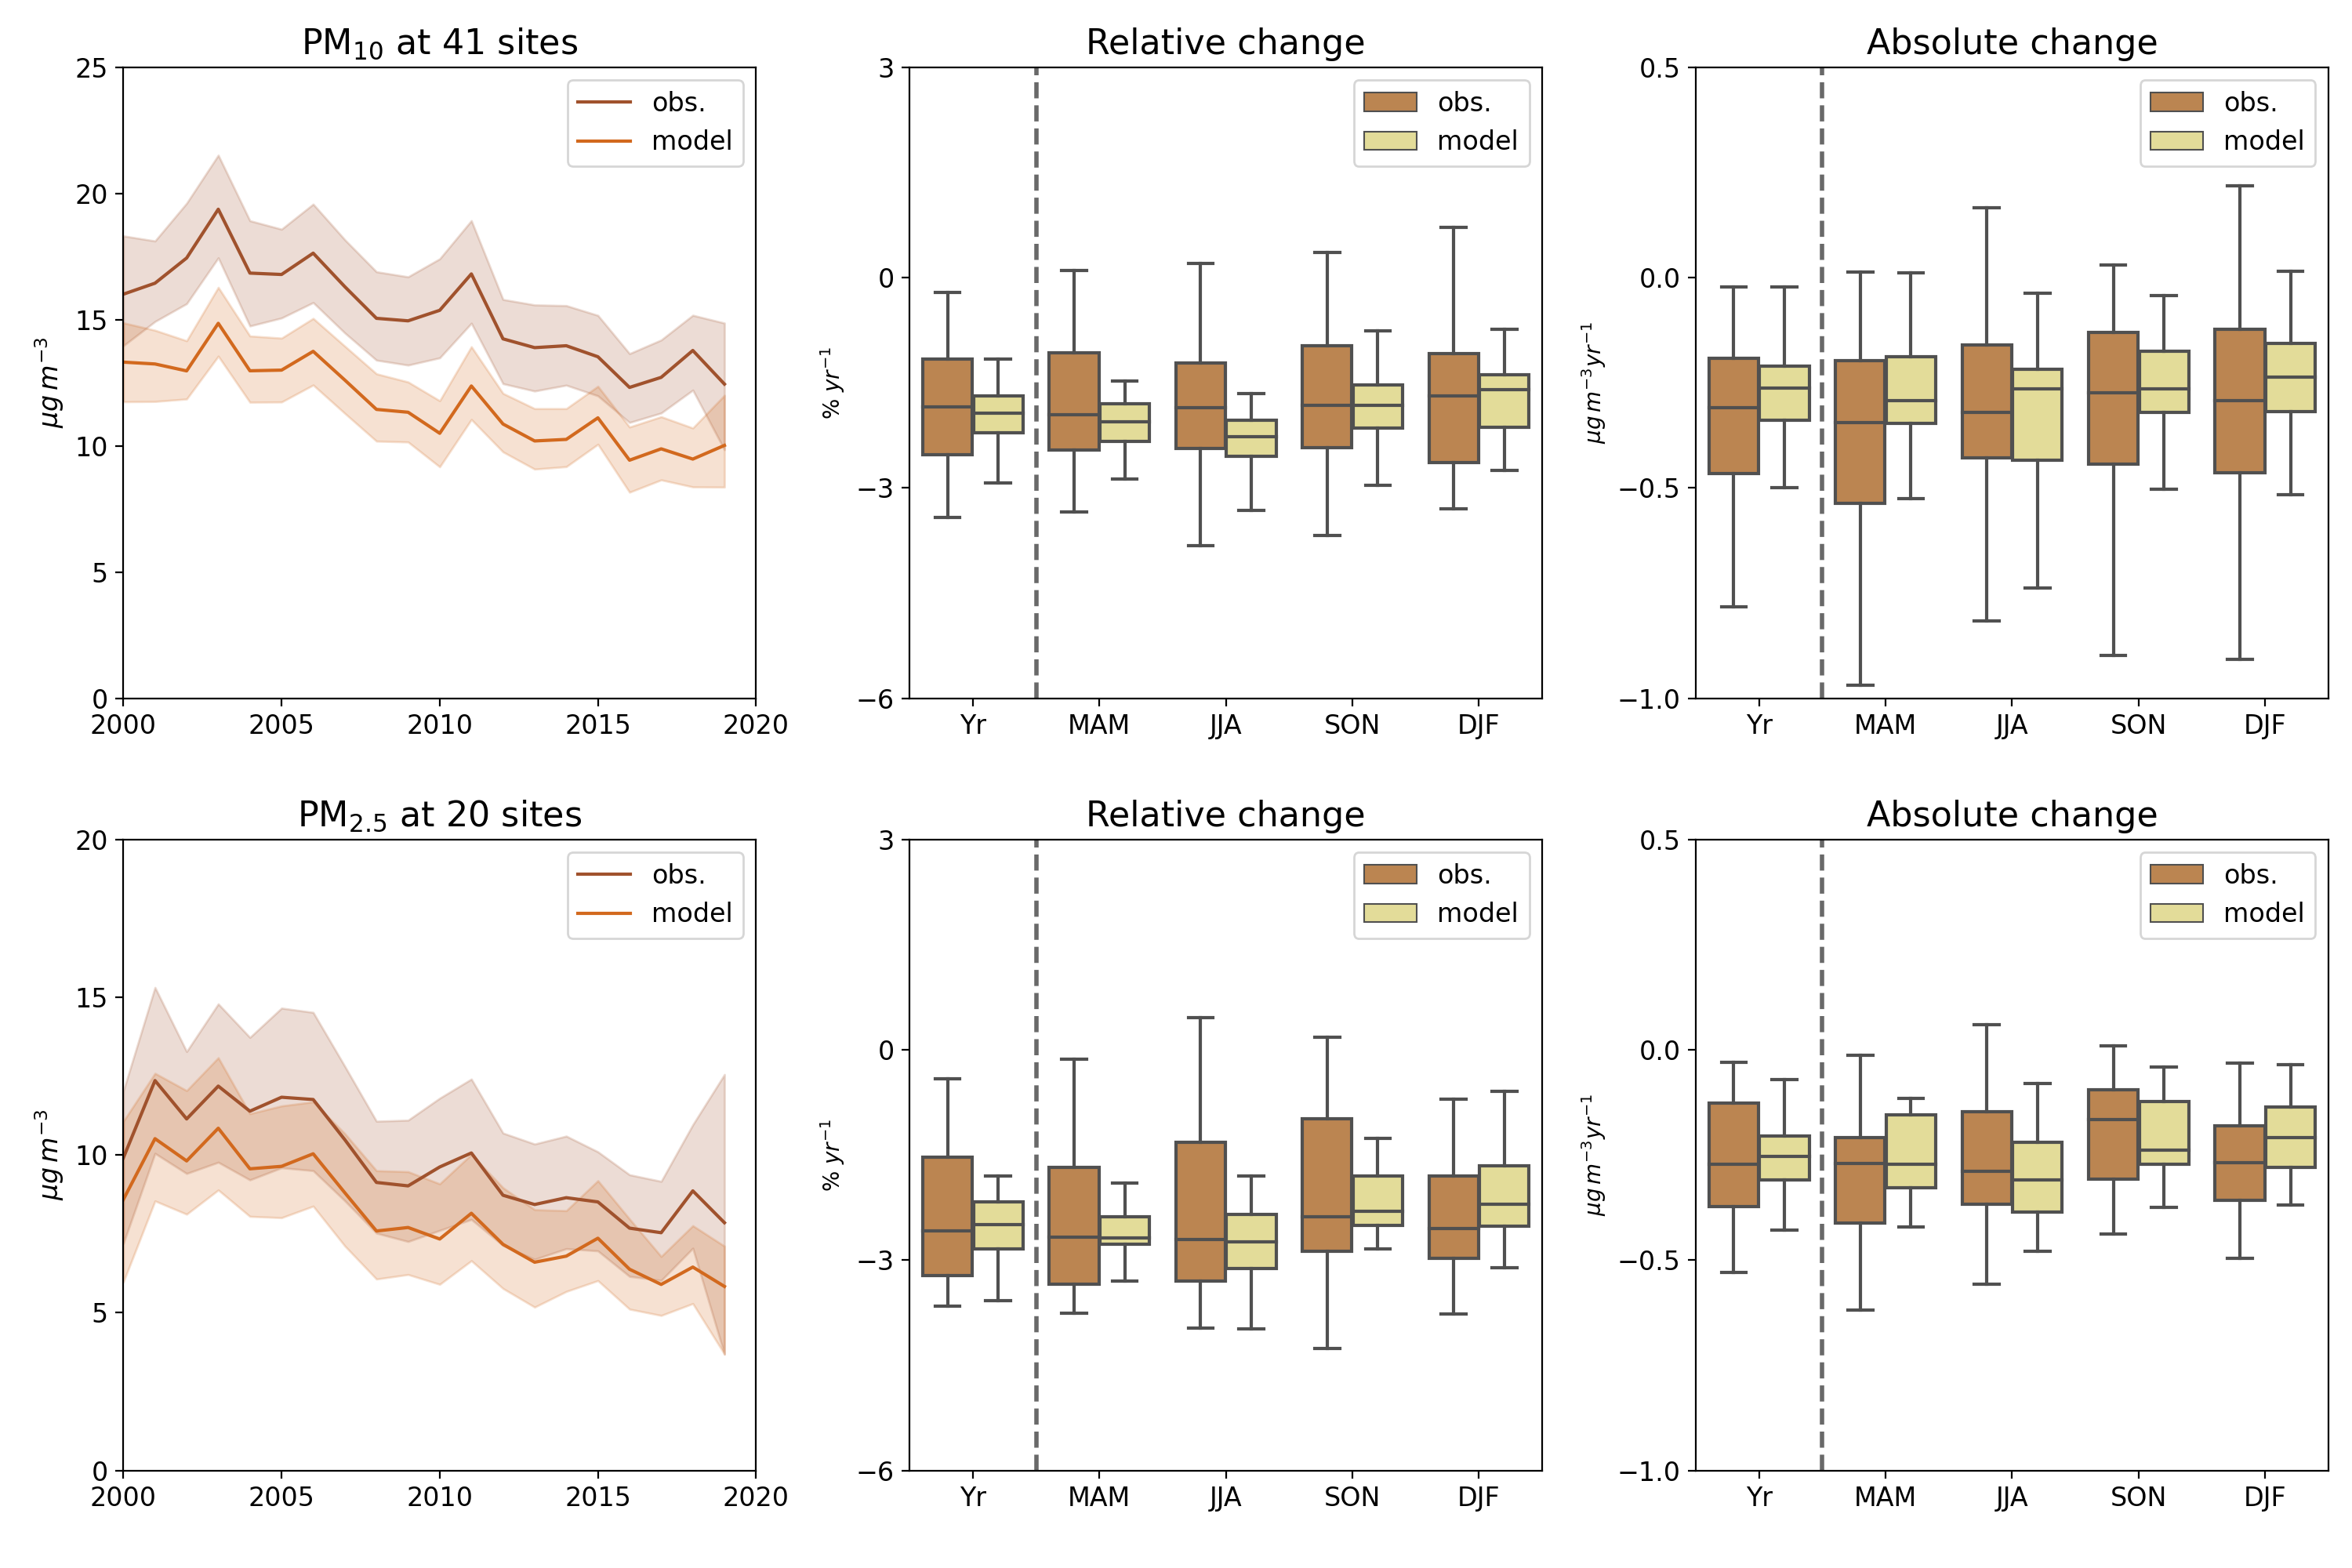
\includegraphics[width=0.74\paperwidth]{FIGS_TRENDS/PM_trends.png}
	\caption{\label{fig:pm_trends}Trends in \PM[10]  and \PM[2.5] from 2010-2019 for EMEP observations and model: left panels - annual timeseries (the solid line indicates the average annual mean trend for all sites, the shaded area shows the 95 \% confidence interval); middle and right panels - relative and absolute trends for all the sites, with both significant and not significant trends (the boxes represent the 50,25,75 percentiles, the whiskers lie within the 1.5 inter-quartile ranges, the mean trends are indicated with black circles}
\end{figure}


\begin{table}
\caption{\label{tab:pm10_stat} Absolute and relative change and corresponding 95\% confidence intervals in observed and modelled annual and seasonal aggregated concentration of \PM[10] for the different time periods. The number of sites with a significant outcome is provided.}
\begin{center}
\scalebox{0.65}{%
\begin{tabular}{ll|ccc|cccc|cccc}
\toprule
          &        & \multicolumn{3}{c}{Number of sites} & \multicolumn{4}{c}{Absolute change (\ug $yr^{-1})$} & \multicolumn{4}{c}{Relative change (\% $yr^{-1}$)} \\
Period & Seasons &           total & sign.(obs.) & sign.(mod.) &                    obs. &          conf.interval &  mod. &          conf.interval &                     obs. &         conf.interval &  mod. &        conf.interval \\
\midrule
2000-2019 & all &              37 &          29 &          36 &                   -0.36 &  (-0.43, -0.29) & -0.29 &  (-0.32, -0.25) &                    -1.83 &  (-2.09, -1.57) & -1.95 &  (-2.11, -1.79) \\
          & winter &              34 &          18 &          20 &                   -0.36 &  (-0.47, -0.25) & -0.26 &  (-0.31, -0.21) &                    -1.73 &   (-2.07, -1.4) & -1.64 &  (-1.83, -1.45) \\
          & spring &              34 &          24 &          32 &                   -0.39 &  (-0.47, -0.31) & -0.30 &  (-0.35, -0.25) &                    -1.84 &  (-2.11, -1.56) & -2.10 &   (-2.29, -1.9) \\
          & summer &              36 &          27 &          31 &                   -0.34 &  (-0.42, -0.25) & -0.32 &  (-0.37, -0.26) &                    -1.72 &  (-2.09, -1.35) & -2.25 &  (-2.47, -2.03) \\
          & autumn &              35 &          22 &          29 &                   -0.34 &  (-0.42, -0.26) & -0.30 &  (-0.34, -0.26) &                    -1.81 &   (-2.1, -1.51) & -1.91 &  (-2.09, -1.74) \\
2005-2019 & all &              54 &          29 &          38 &                   -0.33 &  (-0.41, -0.25) & -0.23 &  (-0.27, -0.19) &                    -1.82 &  (-2.23, -1.41) & -1.79 &  (-2.07, -1.51) \\
2010-2019 & all &              56 &          17 &          23 &                   -0.32 &  (-0.42, -0.21) & -0.16 &  (-0.21, -0.11) &                    -1.84 &  (-2.45, -1.23) & -1.38 &  (-1.81, -0.95) \\
2000-2010 & all &              36 &          14 &          24 &                   -0.46 &  (-0.56, -0.36) & -0.35 &  (-0.46, -0.24) &                    -2.36 &  (-2.77, -1.95) & -2.40 &  (-2.97, -1.83) \\
\bottomrule
\end{tabular}}
\end{center}
\end{table}


\begin{table}
\caption{\label{tab:pm25_stat} Absolute and relative change and corresponding 95\% confidence intervals in observed and modelled annual and seasonal aggregated concentration of \PM[25] for the different time periods. The number of sites with a significant outcome is provided.}
\begin{center}
\scalebox{0.65}{%
\begin{tabular}{ll|ccc|cccc|cccc}
\toprule
          &        & \multicolumn{3}{c}{Number of sites} & \multicolumn{4}{c}{Absolute change (\ug $yr^{-1})$} & \multicolumn{4}{c}{Relative change (\% $yr^{-1}$)} \\
Period & Seasons &           total & sign.(obs.) & sign.(mod.) &                    obs. &          conf.interval &  mod. &          conf.interval &                     obs. &         conf.interval &  mod. &        conf.interval \\
\midrule
2000-2019 & all &              19 &          16 &          19 &                   -0.29 &   (-0.39, -0.2) & -0.26 &  (-0.31, -0.22) &                    -2.42 &   (-2.84, -2.0) & -2.52 &  (-2.71, -2.32) \\
          & winter &              18 &          12 &          12 &                   -0.36 &  (-0.54, -0.18) & -0.21 &  (-0.25, -0.17) &                    -2.29 &  (-2.74, -1.85) & -2.08 &  (-2.35, -1.82) \\
          & spring &              19 &          14 &          19 &                   -0.32 &  (-0.41, -0.24) & -0.27 &  (-0.31, -0.22) &                    -2.47 &  (-2.91, -2.03) & -2.69 &  (-2.88, -2.51) \\
          & summer &              18 &          14 &          17 &                   -0.26 &  (-0.33, -0.19) & -0.30 &  (-0.36, -0.23) &                    -2.36 &  (-2.91, -1.82) & -2.81 &  (-3.16, -2.47) \\
          & autumn &              18 &          12 &          16 &                   -0.26 &  (-0.36, -0.15) & -0.26 &  (-0.33, -0.18) &                    -2.22 &  (-2.71, -1.74) & -2.29 &   (-2.5, -2.07) \\
2005-2019 & all &              36 &          23 &          28 &                   -0.33 &  (-0.42, -0.23) & -0.21 &  (-0.25, -0.17) &                    -2.66 &  (-3.16, -2.16) & -2.28 &  (-2.55, -2.01) \\
2010-2019 & all &              43 &          20 &          19 &                   -0.34 &  (-0.43, -0.25) & -0.18 &  (-0.23, -0.13) &                    -3.14 &   (-3.7, -2.57) & -2.21 &  (-2.67, -1.74) \\
2000-2010 & all &              20 &           7 &          12 &                   -0.36 &   (-0.5, -0.21) & -0.36 &  (-0.46, -0.26) &                    -2.65 &  (-3.56, -1.73) & -2.93 &  (-3.58, -2.27) \\

\bottomrule
\end{tabular}}
\end{center}
\end{table}



\begin{figure}  %DS[H]
  \centering{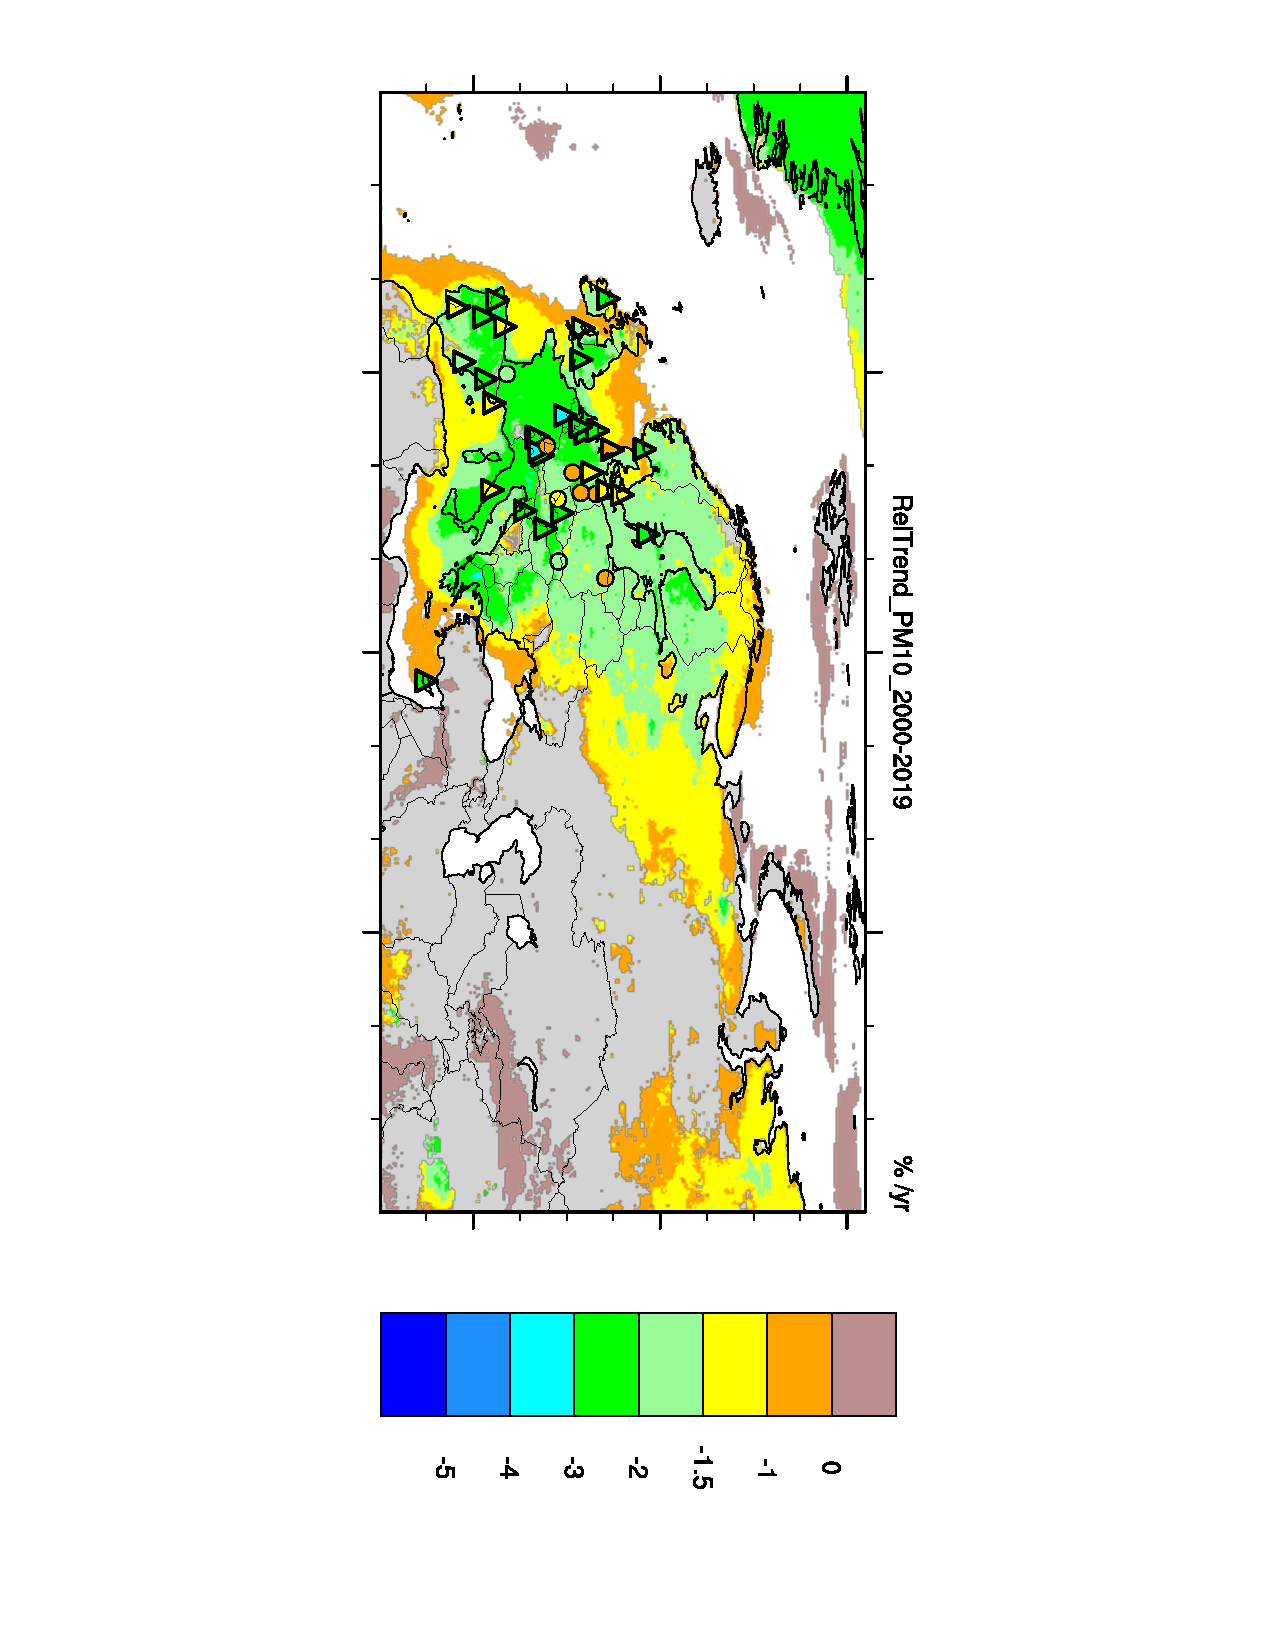
\includegraphics[clip=,angle=90,height=6.1cm,viewport=175 67 448 754]{FIGS_TRENDS/RelTrend_PM10_2000-2019_Perc.pdf}}\\
%  \vspace{0.5cm}
  \centering{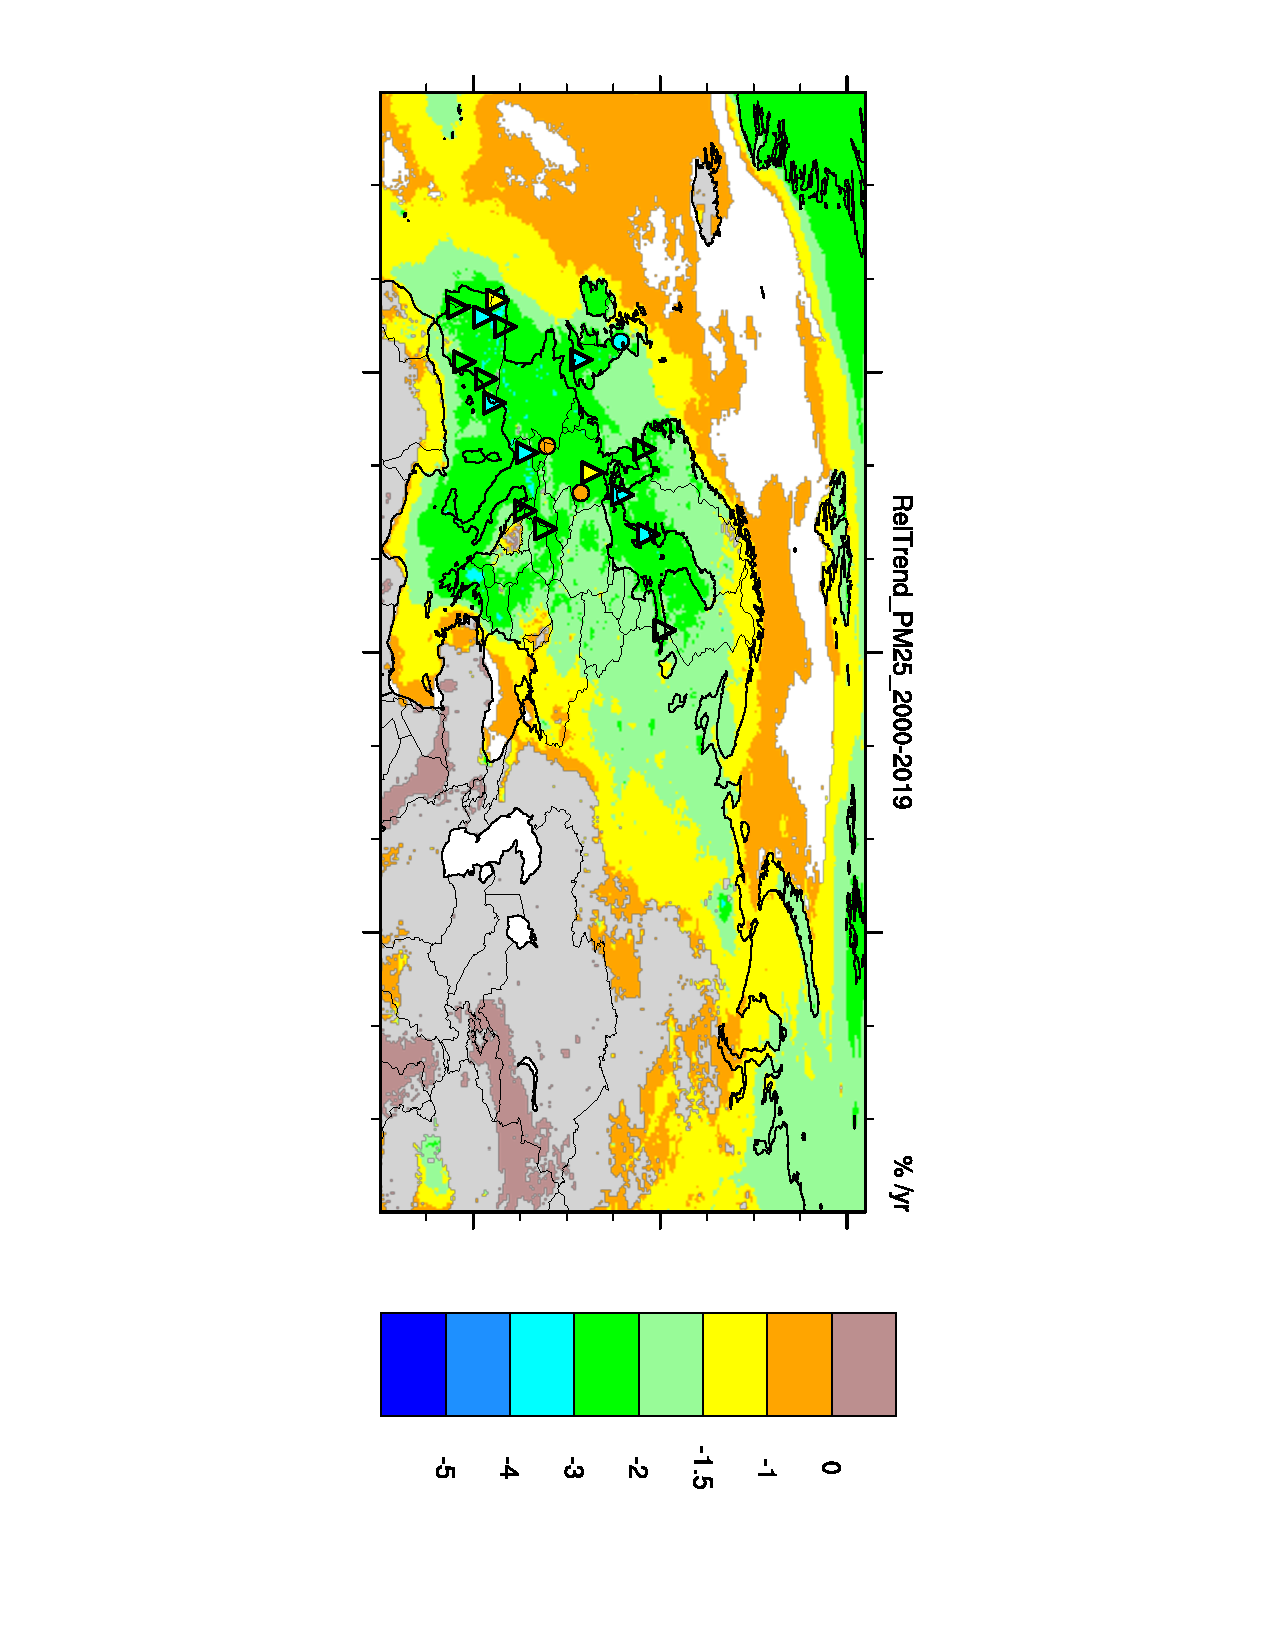
\includegraphics[clip=,angle=90,height=6.1cm,viewport=175 67 448 754]{FIGS_TRENDS/RelTrend_PM25_2000-2019_Perc.pdf}}
\caption{Relative trends for \PM[10] and \PM[2.5] in the period of 2000-2019: EMEP modelled -- coloured contours (grey/white means non-significant trends) and observed - coloured triangles (significant) and circles (non-significant).}
\label{fig:PMtrends}
\end{figure}


For the whole period, 36 and 18 sites with satisfactory data coverage have been included in the trend analysis respectively for \PM[10] and \PM[2.5]. The annual series of \PM[10] and \PM[2.5] clearly show a general concentration decrease from 2000 to 2019. In general, the model underestimates the concentrations, but reproduces quite well observed year-to-year changes in \PM[10] and \PM[2.5], including enhanced PM levels due to meteorological conditions e.g. in 2003 (dry hot summer \citep{EMEP:PM2005}) and 2011 (dry year in Western/Central/Southern Europe \citep{EMEP:PM2013}).


For the period of 2000-2019, the average observed \PM[10] trends are -0.36 \ug $yr^{-1}$, or -1.83 \% $yr^{-1}$ in relative terms. The corresponding \PM[10] trends from model simulations are -0.27 \ug $yr^{-1}$ and -1.92 \% $yr^{-1}$. For \PM[2.5], the average absolute trends are -0.29 and -0.25 \ug $yr^{-1}$ and the relative ones are -2.42 and -2.51 \% $yr^{-1}$, observed and modelled respectively. The reduction of anthropogenic emissions during this period is a major cause for the decreasing average concentrations of PM, with \PM[10] trends experiencing larger disturbances due to considerable contribution from natural aerosols of sea salt and mineral dust in the coarse fraction. Considerable changes in PM pollution caused by the inter-annual meteorological variability also interfere with the PM trends due to emission changes, as the weather conditions affect both the formation of secondary aerosols, emissions of natural particles, and dry and wet depositions.


Figure \ref{fig:pm_trends} reveals a considerably larger variation of observed trends between the sites in comparison to modelled trends, still with modelled median (and mean) trends lying within 25-75\% inter-quartile range (IQR) of the observed ones. A larger spatial variability of observed trends with respect to model simulated ones can also be seen on the maps of relative trends in Figure \ref{fig:pm_trends}. The largest decreases in \PM[10] were observed at the French site (FR0009) by 3.4 \% $yr^{-1}$ and at the Swiss (CH0005) by 3.1 \% $yr^{-1}$. and the smallest, below 1\%, in Germany and Poland. For \PM[2.5], decrease larger than -3 \% $yr^{-1}$ was observed at 8 out of 19 sites, situated in Sweden, Norway, the UK, Spain, the Po Valley, and in Austria, while the smallest decreasing trends were as for \PM[10] registered at German sites. The modelled \PM[10] and \PM[2.5] trends are between -1.5 and -2.5 \% $yr^{-1}$ for most of Europe (with the largest decrease of \PM[2.5] between -2.5 and -3 \% $yr^{-1}$ in France). Most of the sites, for which the observations estimate insignificant trends, are located in Central Europe (mostly in Germany). The modelled trends are mostly significant and ranging between -1 and -3 \% over practically all European part of EMEP.

The observations and model simulations indicate more sites with significant trends and larger \PM[10] and \PM[2.5] average decreases for the warm seasons. For the cold seasons, when PM pollution is typically more serious, the relative decreasing trends are in general smaller, and the number of sites with non-significant trends is larger, which is especially pronounced for observed \PM[10] trends.

PM is a complex pollutant, consisting of aerosol species both emitted
directly and formed from gaseous precursors.Therefore, the reductions both in primary PM emissions, as well as \sox, \noii, \nhiii and NMVOC emissions are contribute to decrease PM concentrations. In the western parts of EMEP (EU \&UK \&EFTA), where the considered sites are located, the emissions of primary \PM[10] and \PM[2.5] were reduced by 32 and 35 \%, respectively, from 2000 to 2019. The largest in the same period was the reduction in \sox emissions (81 \%), resulting in 61 \% observed decrease of \soiv (70 \% according to the model). Following the reduction of \noii emissions by 48 \%, observed \noiii concentrations decreased slightly less, i.e. by 38 \% (44 \% according to the model). This was partly due to a rather moderate reduction by 12 \% in \nhiii emissions and the availability of free \nhiii due to the reduced formation of ammonium sulphate. 

\COMMENT{Though \noii was reduced by 48 \%, given the moderate reduction by 12 \% in \nhiii emissions and the availability of free \nhiii due to the reduced formation of ammonium sulphate, the observed decrease in \noiii concentrations was only 38 \% (44 \% by the model).}
 The corresponding changes from 2000 to 2019 in \nhiv were 50 and 48 \%. Due to the lack of consistent observational data for carbonaceous aerosols in the 2000s, the trends of elemental (EC) and organic (OC) carbon have only been analysed for a 2010-2019 period (see discussion in \ref{sec:trendsECOC}). The examples of the changes in the chemical composition of \PM[2.5] from 2000(2002) to 2019 are given on Figure \ref{fig:KEX4} for the only six sites with enough measurements for deriving the mass balance. 

Summarizing trend results for the 2000-2019 period, the average \PM[10] and \PM[2.5] trends, derived from observational data and model simulations, are decreasing. Significant trends have been estimated from observational data for 78 \% of sites for \PM[10] and 84 \% of sites for \PM[2.5]; the model simulates significant trends for more sites, namely 97 and 100 \% respectively. During this 20-year period, observed \PM[10] concentrations decreased by 35 \%  (36 \% from model simulations) on average at the considered sites. The average observed decrease of \PM[2.5] is 46 \%  (48 \% estimated by the model). We find quite a good correspondence between observed and model simulated trends in PM concentrations. 

Furthermore, Figure \ref{fig:pmExc_trends} presents 

\begin{figure}
	\centering
	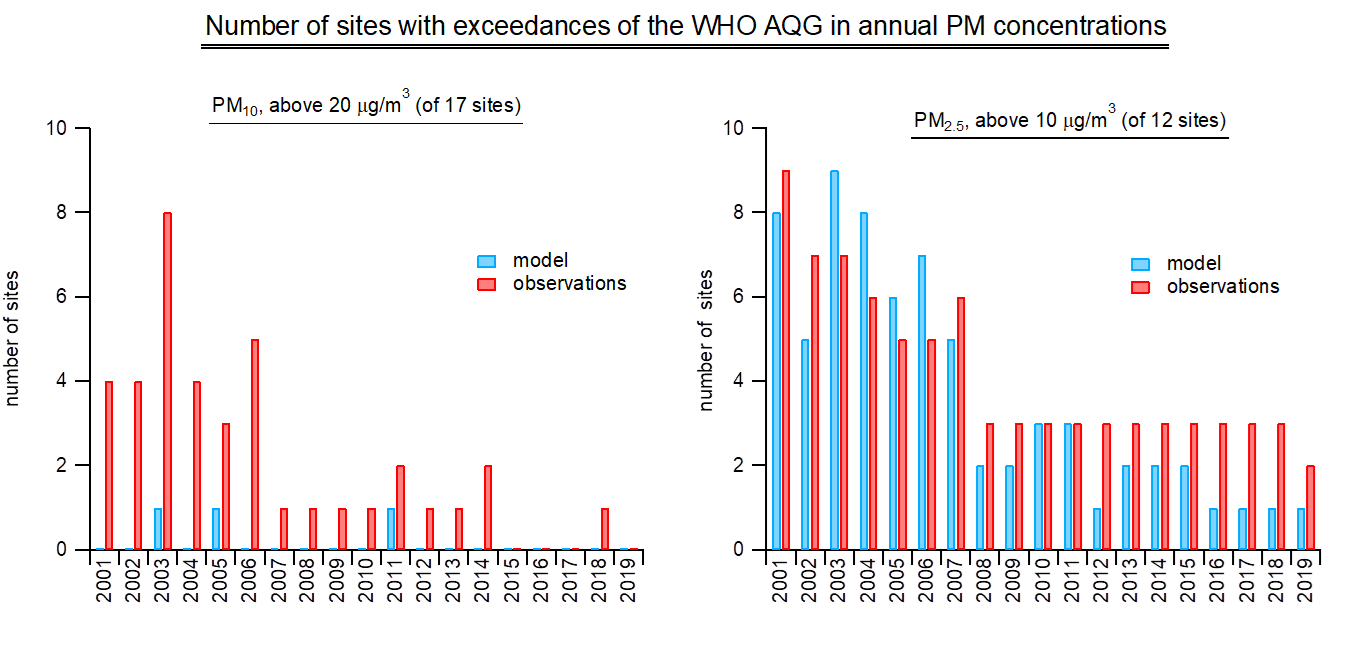
\includegraphics[width=0.74\paperwidth]{FIGS_TRENDS/PM_exceedences_2001-2019.png}
	\caption{\label{fig:pmExc_trends} Number of EMEP sites with exceedances  in \PM[10]  and \PM[2.5] exceedances of WHO AQGs between 2001 and 2019, as observed and modelled with the EMEP MSC-W model}
\end{figure}


\COMMENT{For the period 2005-2019 (starting from the reference year of Gothenburg Protocol), more sites with data coverage were totally available for this \PM[10] and \PM[2.5] trend analysis, i.e. 53 and 35 respectively, but significant trends have been observed and modelled for a smaller fraction of the sites with respect to the 2000-2019 period (partly due to a shorter period length)}


%%%%%%%%%%%%%%%%%%%%%%%%%%%%%%%%%%%%%%%%%%%%%%%%%%%%%%%%%%%%%%%%%%%%%%%%%%%%%%%%%%%%%%%%%%%%%%%%%%%%%%%%
\clearpage
\section{\label{sec:Trends_O3}Trends in O$_3$ }

Trend studies of surface ozone requires a somewhat different approach than other species since ambient ozone levels are the result of a substantial baseline level with episodes on top. 
 Whereas NOx often leads to ozone formation in rural areas in the summer season, it can cause depletion of ozone by titration in and downwind of urban areas, especially in winter.
Thus, the effect of man-made emissions of ozone precursors as NOx (in combination with VOCs) is to change the distribution of hourly and daily ozone concentrations during a year with high ozone levels in the summer half year and low ozone levels in the winter half year. Furthermore, the extent of these perturbations is significantly determined by the weather conditions and thereby by the ongoing climate change. Harmful levels of surface ozone are closely linked to high-pressure situations with elevated temperatures and strong solar radiation.

Thus, the selection of ozone metrics is decisive for the estimated trends \citep[e.g.][]{LefohnTOAR2018}. The annual mean concentration used for evaluating other species is of little interest when studying ozone. A common procedure is to look at the trend in the probability distribution of ozone, e.g. by calculating trends for various percentiles of the distribution \citep[e.g.][]{SimpsonCOSUST2014}.  

As explained above, the trends in six percentiles (10, 50, 75, 95, 98 and 99) of the daily maximum O$_3$ values were calculated for stations with at least 330 valid daily data each year. This corresponds to 90~\% data capture in the individual years. The 10th percentile corresponds to the 37th lowest daily maximum value while the 99th percentile corresponds to the 4th highest daily maximum. 

Figure \ref{fig:O3_boxplot} shows the calculated Sen's slopes for these six percentiles for the period 2000--2019 for EMEP sites north and south of 49\degrees N based on observed and modelled data. Both significant and non-significant slopes were included, but stations above 1200~m altitude were not included in the trend statistics. The reason for differing the altitude criteria for trend calculations vs that for evaluating the 2019 levels as discussed in Ch 2.4 (1200~m vs 500~m) was that the latter is more focused on individual daily data whereas the trends are based on aggregated statistics (annual data). 

For both the observed and modelled data the trends show an increase in the 10th percentile and with a gradually stronger decrease in the higher percentiles. This is as expected when the emission of precursors (NOx) is reduced with time. The increase in the 10th percentile is explained by reduced titration by NOx while the the decreasing trend in the highest percentiles is explained by reduced photochemical formation of ozone in summer. The net result of these trends is a narrowing of the distribution of O$_3$ concentrations. 

Figure \ref{fig:O3_boxplot} shows the trends in annual percentles for sites north and south of 49\degrees N. In general the agreement is rather good, with the model agreeing very well with the observations for the high percentiles for stations N of 49\degrees, though overestimating somewhat the decrease of the high percentiles (95-99) for stations south of 49\degrees N. This is an important finding since these percentiles are the main indicators for surface ozone pollution events. Figure \ref{fig:O3_boxplot} furthermore shows that the spread in the observed data is significantly larger than the spread in modelled data which is as expected. A grid model will inevitably reduce local geographical differences and produce smoothed concentrations fields. 

For the 10th percentile, the model overestimates the increase both north and south of \mbox{49\degrees~N}. It is not obvious what this overestimation is due to. It could reflect that NOx in winter is not reduced as much as the emissions and model assume, or it could e.g. reflect deficiencies in the model description of atmospheric vertical stability and exchange of pollutants in winter. A possible underprediction of European NOx emissions was suggested as a likely cause of model underprediction of peak ozone and over prediction of low ozone by \citet{Oikonomakis2018}.


The relative trends shown in Figure \ref{fig:O3_boxplot} are based on the Sen's slopes and use the value of these trend lines the first year (i.e. in 2000) as the reference for the modelled and observed data separately. The results given in Figure \ref{fig:O3_boxplot} thus show the estimated relative changes without any reference to the absolute levels of the modelled and observed data. 

The trends in the absolute levels are given in Figures \ref{fig:O3_perctrends_N} and \ref{fig:O3_perctrends_S}. Annual O$_3$ percentile values for the observed and modelled data during 2000--2019 are shown in Figures \ref{fig:O3_perctrends_N} and \ref{fig:O3_perctrends_S} for stations north and south of 49\degrees N, respectively. The solid lines mark the mean of all stations while the shaded areas mark the 25th and 75th percentile of these station-based values. All stations below 1200 m asl and with at least 15 years of data were included. 

These results show that the modelled 10th and 50th percentiles are higher than the observations whereas the observed high percentiles (95--99) are higher than modelled. The bias in the high percentiles are particularly strong for stations south of 49\degrees N. For the 75th percentile, the absolute levels of the modelled and observed data agree very well. 

The interannual variation in the higher percentiles, i.e. the change in levels from year to year, is however very well reproduced by the model. Peak years as 2003 and 2006 in both regions as well as 2015 in the south and 2018 and 2019 in the north is reproduced by the model but with a substantial offset. This implies that the episodes leading to the peak values are captured by the model but that the ozone levels during the episodes are underestimated. 

Trends in ozone metrics linked to harmful effects on vegetation (AOT40) and on human health (SOMO35) are shown in Figures \ref{fig:O3_aot40croptrends} - \ref{fig:O3_somo35trends} for sites north and south of 49\degrees N, respectively. The absolute levels of these metrics are very sensitive to the baseline O$_3$ concentration level \citep{SofievTuovinen} which is close to the 35--40 ppb range. Thus, comparisons between modelled and observed data can be difficult (though as shown in SI Fig.S6, \citealt{Etzold:2020}, the EMEP model can often reproduce AOT40 quite well). 

Figures \ref{fig:O3_aot40croptrends} and \ref{fig:O3_aot40foresttrends} show a clear underestimation by the model compared to the observed data, in particular for the southern sites. Both the modelled and observed data do however indicate a marked decreasing trend during 2000--2019. For SOMO35 (Fig.\ref{fig:O3_somo35trends}), the model calculations agree very well with the observed data, both with respect to the absolute levels and the trends. For the southern sites, a slight underestimation is seen in the peak years (2003 and 2018) though. 

Summary statistics for the observed and modelled trends during 2000-2019 for the 75th and 99th percentiles as well as SOMO35, AOT40 for crops and AOT40 for forests are given in Table~\ref{tab:O3_stat} for sites north and south of 49\degrees N. These data show the mean trend (as absolute values and relative to 2000 in percent) as calculated by the Theil-Sen's slope. The slopes for the percentiles were calculated by the pyaerocom tool as explained above while the slopes for SOMO35 and AOT40 were calculated by the R libraries 'Kendall' and 'zyp'. 

In addition to the mean trends, the confidence intervals for these mean values are also given. The confidence intervals were computed by standard bootstrapping techniques \citep{DavisonHinkley:1997} using the R library 'boot' (basic bootstrap method with 1000 resamples). Various bootstrap method were tested out and compared to direct calculations of the confidence intervals based on the sample mean and sample standard deviation. These comparisons showed that the various methods produced very similar estimates of the confidence intervals for the mean values and thus we conclude that the confidence intervals for the means are fairly robust. These confidence intervals could be used to judge if the mean observed trends differ from the mean modelled trends.



First of all, it is interesting to note that downward trends are found for all the five metrics both north and south of 49\degrees N and for both observed and modelled data. This is a strong signal that there has been a real reduction in these ozone metrics during the 2000-2019 period. Furthermore, for sites north of 49\degrees N, the results indicate that there are no significant difference between the observed and modelled trends in the 75th and 99th percentiles. For sites south of 49\degrees N the mean absolute trends agree very well for the observed and modelled data, but the relative changes in the observations are clearly lower than the modelled changes (reflecting that the model underpredicts the absolute level of the high percentiles). It could be noted that the number of statistically significant trends are considerably lower for the observed data compared to the modelled ones. 

For SOMO35 and AOT40 the number of sites with significant trends in the observations are rather low and substantially lower than the number of statistically significant modelled trends. For all three metrics the model calculates stronger mean reductions than observed. For SOMO35 north of 49 \degrees N, the mean observed and modelled absolute trends are very close, but the modelled relative trend is somewhat larger than observed.




\begin{table}
\caption{\label{tab:O3_stat} The estimated mean values of the absolute and relative trends (2000--2019) in O$_3$ metrics based on stations north and south of 49\degrees N (observed and modelled). The corresponding 95\% confidence intervals of these mean values and the number of sites with significant trends are also provided. Results are given for the 75th and 99th percentile as well as SOMO35, EU definition of AOT40 for crops (AOT40c), and EU definition for forests (AOT40f). Note that the number of sites 'obs' and 'mod' refer to the number of sites with significant slopes (p<0.05) whereas the man values include all sites irrespective of the significance.}
\begin{center}
\scalebox{0.65}{%
\begin{tabular}{Hll|ccc|cccc|cccc}
\toprule
          &    &    & \multicolumn{3}{c}{Number of sites} & \multicolumn{4}{c}{Absolute change (ppb)} & \multicolumn{4}{c}{Relative change (\% $yr^{-1}$)} \\
Period & Area & Parameter &           total & obs & mod &                    obs. &          conf.interval &  mod. &          conf.interval &                     obs. &         conf.interval &  mod. &        conf.interval \\
\midrule
2000-2019 & N of 49N & 75p &  52 &  19 &  30 & -0.15 & (-0.19, -0.10) & -0.13 & (-0.14, -0.10) & -0.31 & (-0.40, -0.21) & -0.26 & (-0.30, -0.22) \\
2000-2019 & N of 49N & 99p &  52 &  13 &  39 & -0.41 & (-0.48, -0.33) & -0.34 & (-0.37, -0.30) & -0.58 & (-0.68, -0.47) & -0.54 & (-0.59, -0.49) \\
2000-2019 & N of 49N & SOMO35 &  55 &   9 &  33 & -18.29 & (-26.3, -11.2) & -17.92 & (-21.1, -14.7) & -0.54 & (-1.41, 0.021) & -0.85 & (-1.02, -0.70) \\
2000-2019 & N of 49N & AOT40c &  55 &  12 &  42 & -71.63 & (-91.2, -52.4) & -153.35 & (-175., -132.) & -1.35 & (-2.03, -0.73) & -2.10 & (-2.32, -1.88) \\
2000-2019 & N of 49N & AOT40f &  55 &   9 &  43 & -121.11 & (-156., -85.5) & -220.10 & (-250., -191.) & -1.10 & (-1.86, -0.47) & -1.75 & (-1.92, -1.56) \\
\\
2000-2019 & S of 49N & 75p &  40 &  16 &  38 & -0.20 & (-0.27, -0.13) & -0.26 & (-0.27, -0.23) & -0.35 & (-0.46, -0.21) & -0.46 & (-0.49, -0.43) \\
2000-2019 & S of 49N & 99p &  40 &  18 &  37 & -0.48 & (-0.59, -0.36) & -0.51 & (-0.54, -0.46) & -0.57 & (-0.71, -0.43) & -0.70 & (-0.74, -0.65) \\
2000-2019 & S of 49N & SOMO35 &  35 &  14 &  31 & -36.74 & (-54.9, -18.6) & -40.59 & (-45.3, -36.2) & -0.77 & (-1.27, -0.28) & -1.12 & (-1.23, -1.01) \\
2000-2019 & S of 49N & EUAOT40c &  35 &  13 &  33 & -190.26 & (-247., -128.) & -286.65 & (-313., -260.) & -1.49 & (-1.97, -1.02) & -1.98 & (-2.17, -1.80) \\
2000-2019 & S of 49N & EUAOT40f &  35 &  16 &  31 & -312.64 & (-422., -196.) & -480.46 & (-537., -425.) & -1.36 & (-1.87, -0.85) & -1.74 & (-1.94, -1.55) \\
\bottomrule
\end{tabular}}
\end{center}
\end{table}




\begin{figure}[h]
	\centering
	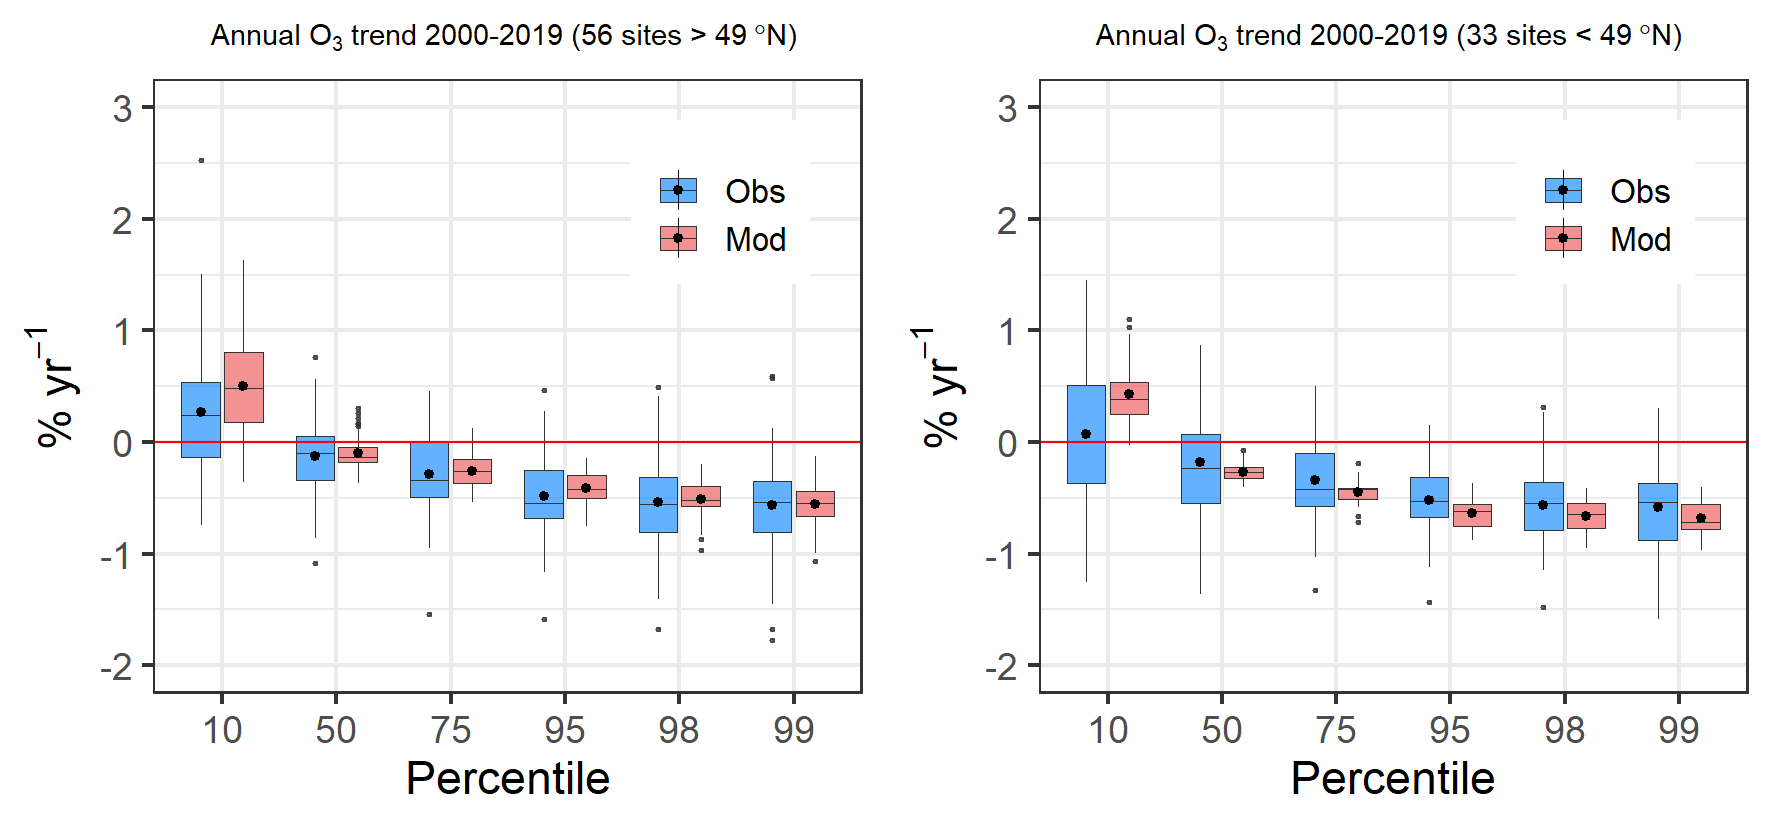
\includegraphics[width=0.74\paperwidth]{FIGS_TRENDS/O3_boxpl.png}
	\caption{\label{fig:O3_boxplot}Boxplot of trends in annual percentiles of daily max O$_3$ from 2000--2019 for EMEP observations and model calculations for stations north (left) and south (right) of 49\degrees N. The boxes mark the 25 and the 75 percentiles with the median given as a thin line inside. The upper whisker extends from the hinge to the highest value that is within 1.5*IQR of the hinge, where IQR is the inter-quartile range, or distance between the first and third quartiles. The lower whisker extends from the hinge to the lowest value within 1.5*IQR of the hinge. Data beyond the end of the whiskers are outliers and plotted as points. The mean values are shown as black circles. Both significant and non-significant trend values were included. Only sites below 1200 m asl and with at least 15 years of data are included.}
\end{figure}

\begin{figure}[h]
	\centering
	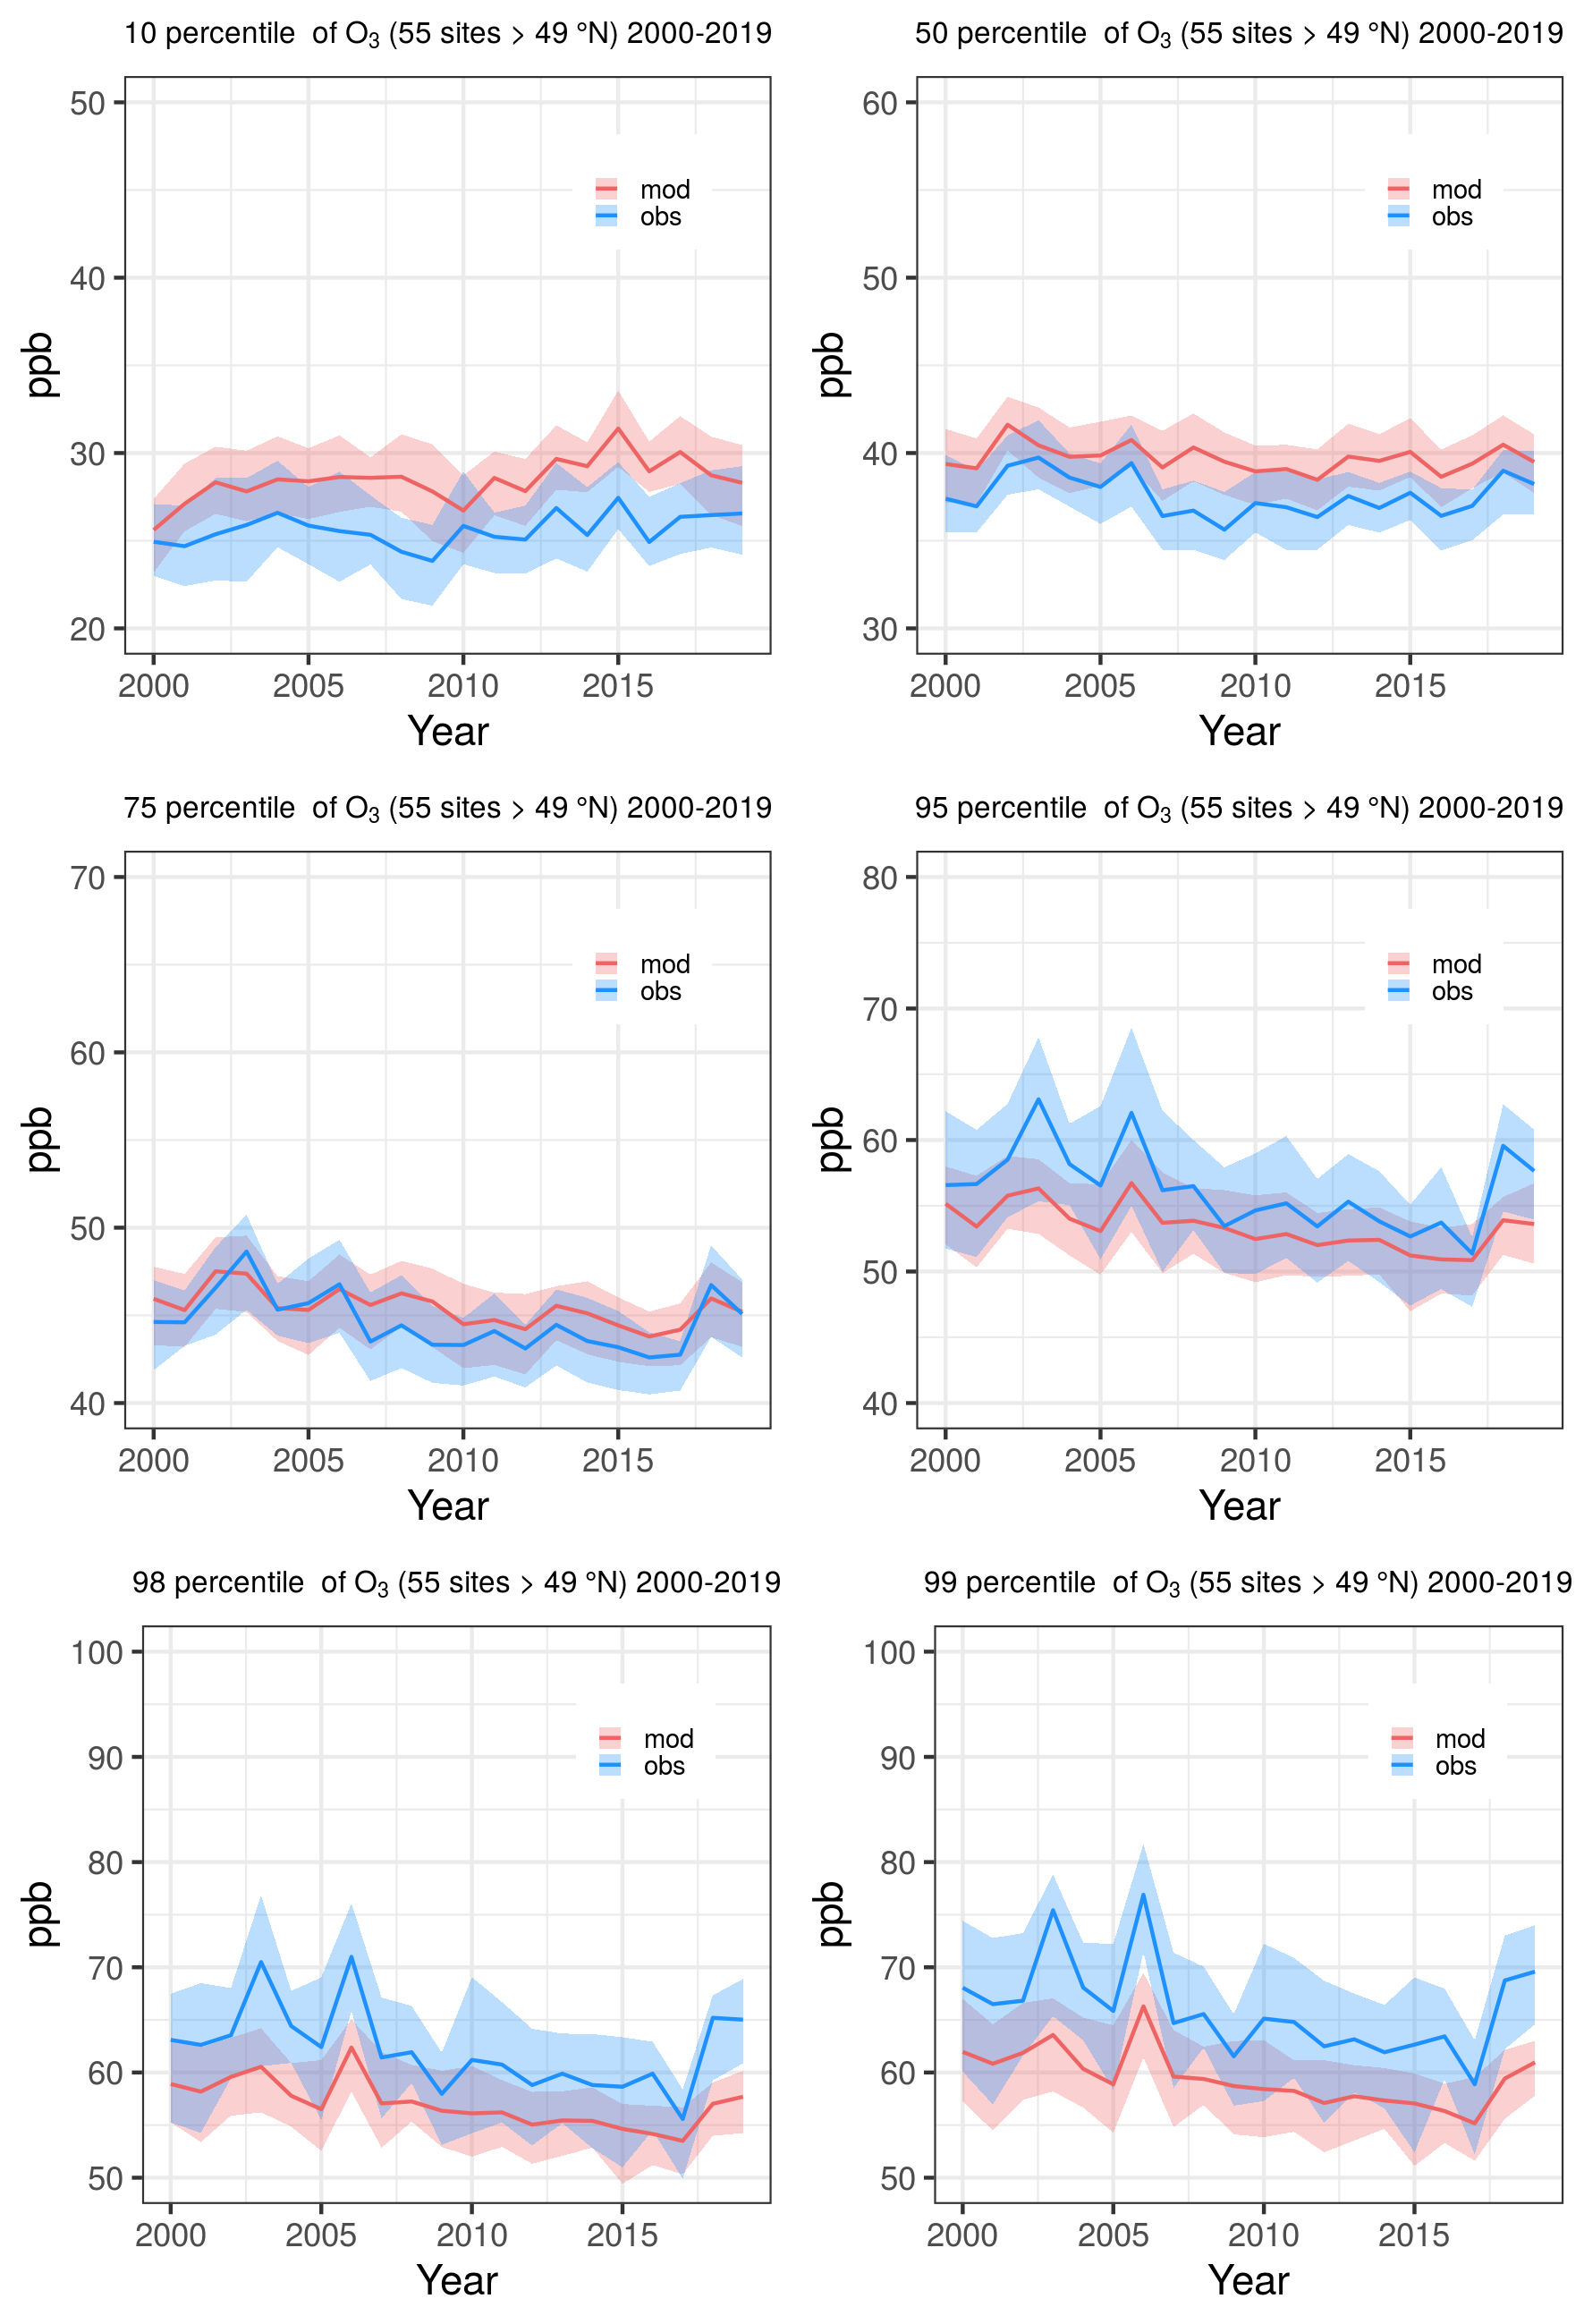
\includegraphics[width=0.74\paperwidth]{FIGS_TRENDS/alltrends_north_49_2000_2019_1200m.png}
	\caption{\label{fig:O3_perctrends_N}Trends in annual percentiles of daily max O$_3$ from 2000--2019 for EMEP observations and model calculations for sites north of 49\degrees N: The solid line indicates the mean, and the shaded area marks the 25th and 75th percentile. Only sites below 1200 m asl and with at least 15 years of data are included.}
\end{figure}

\begin{figure}[h]
	\centering
	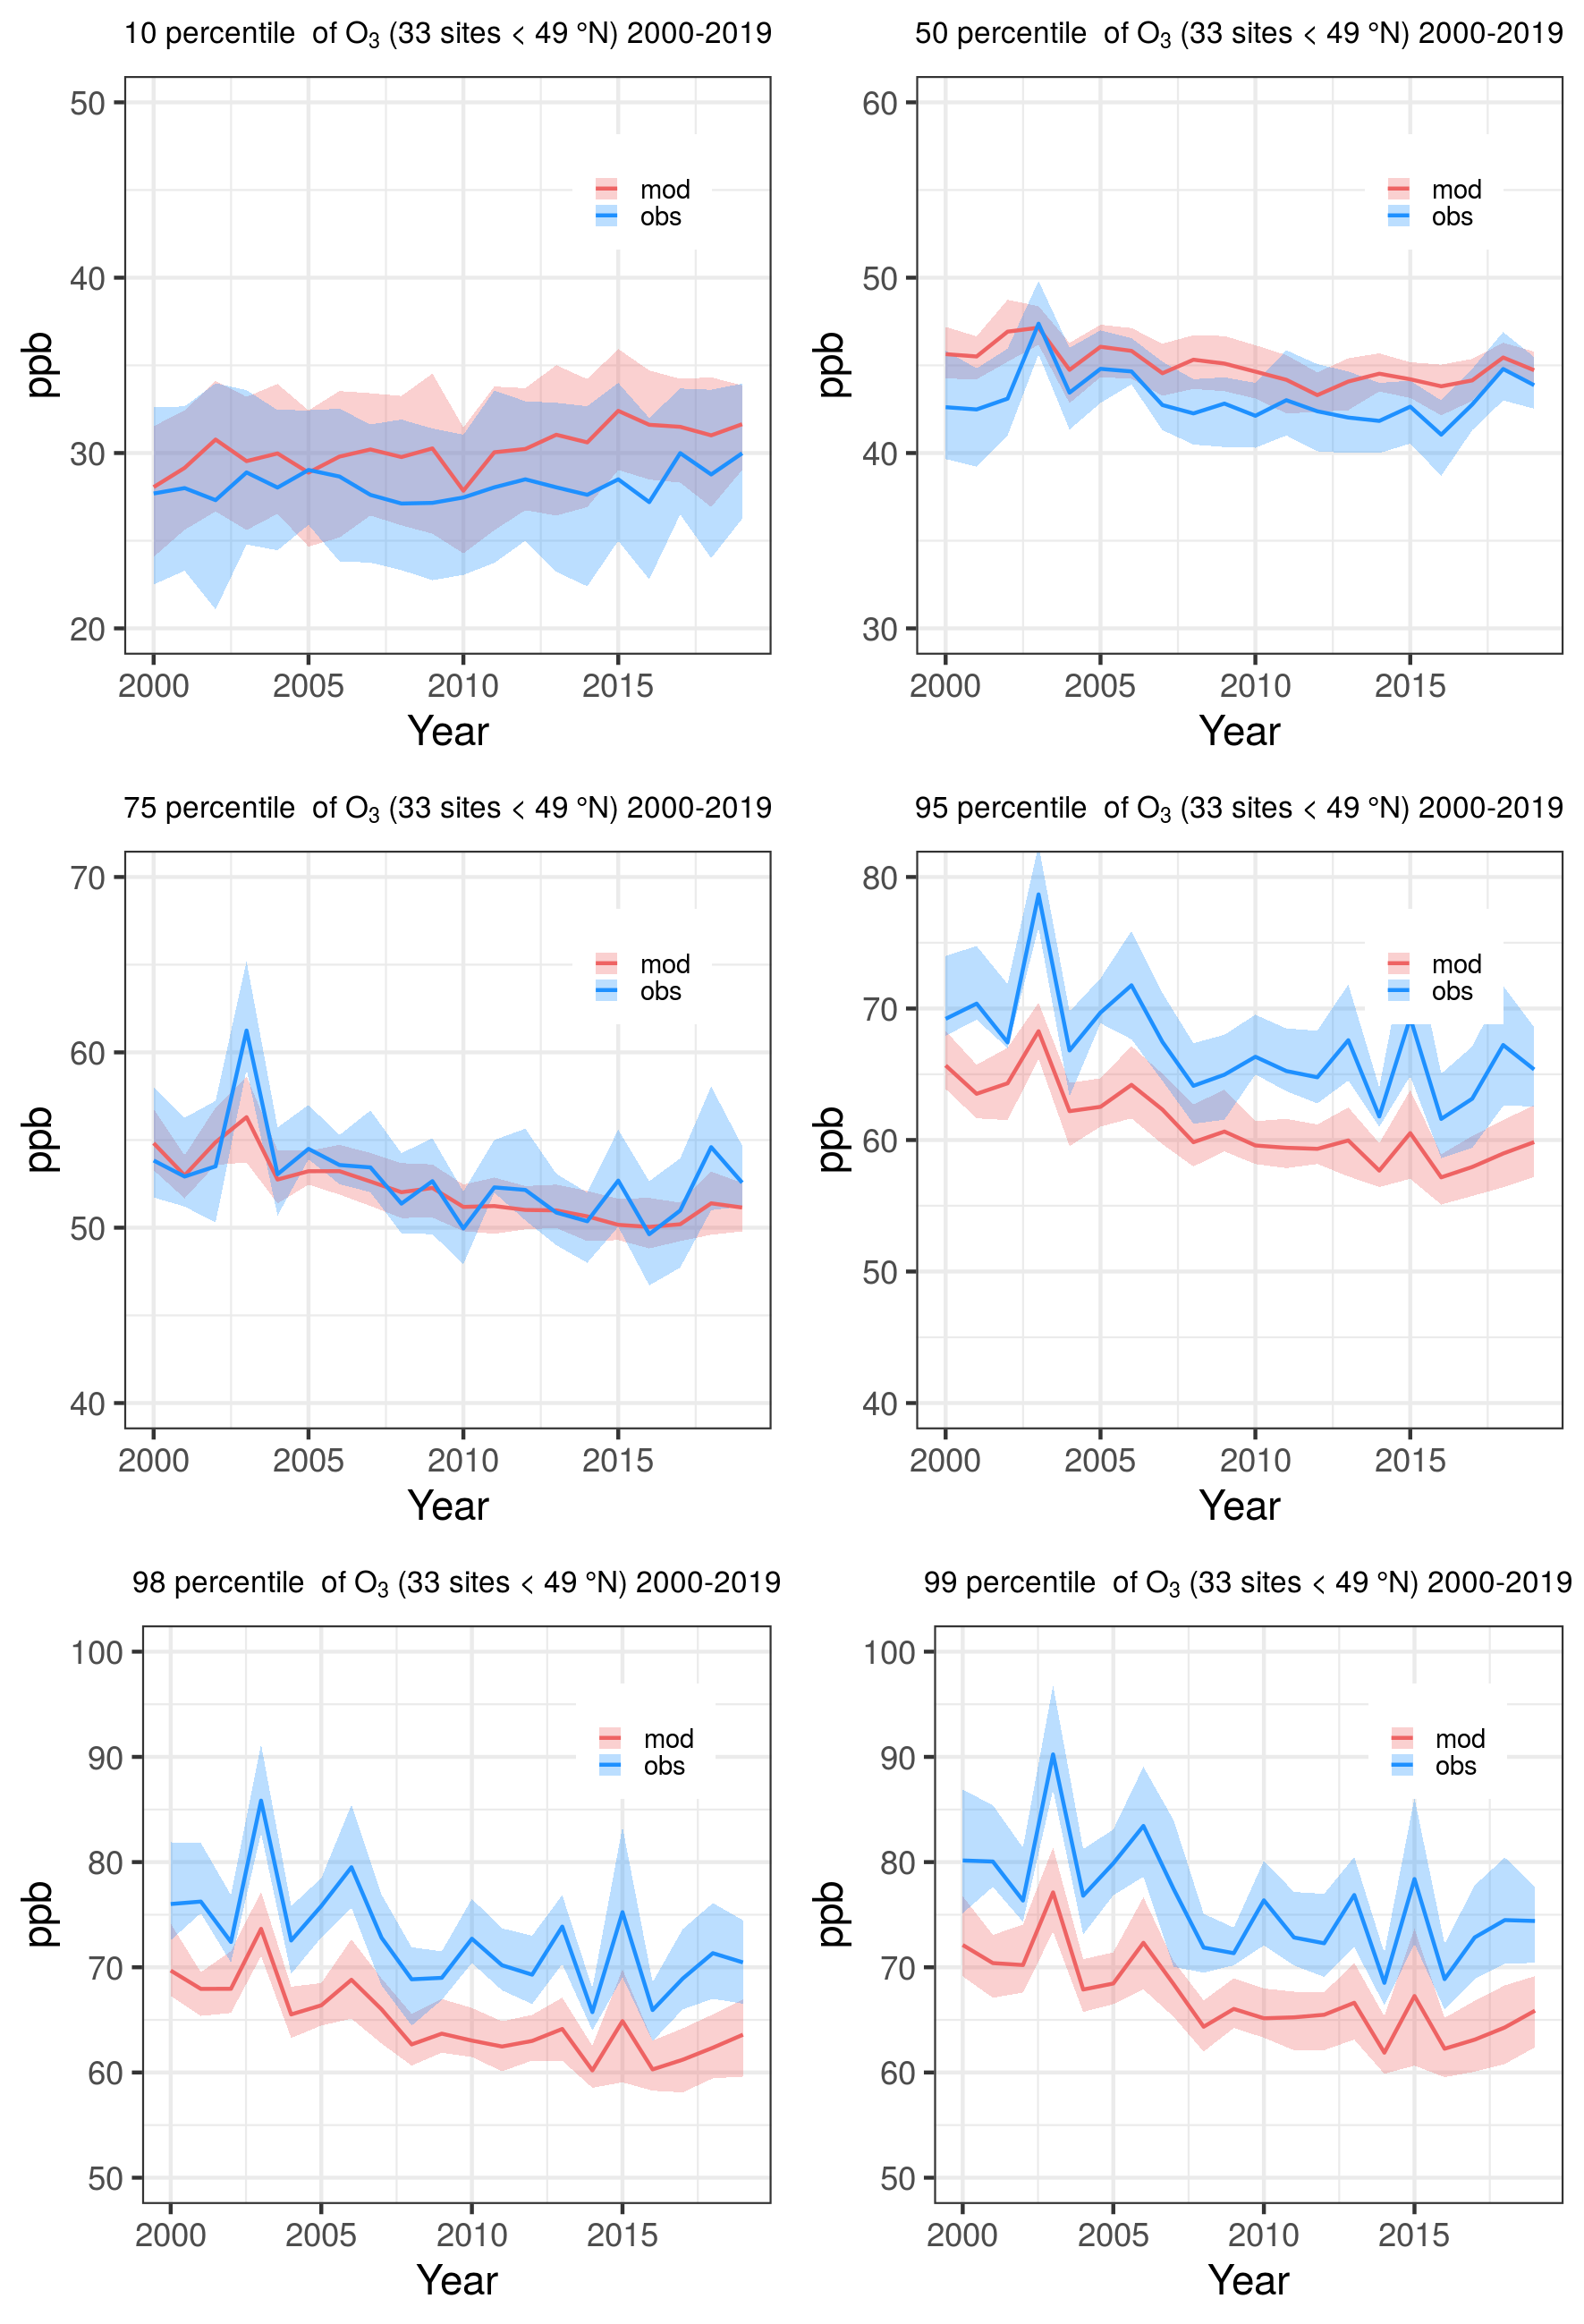
\includegraphics[width=0.74\paperwidth]{FIGS_TRENDS/alltrends_south_49_2000_2019_1200m.png}
	\caption{\label{fig:O3_perctrends_S}Trends in annual percentiles of daily max O$_3$ from 2000--2019 for EMEP observations and model calculations for sites south of 49\degrees N: The solid line indicates the mean, and the shaded area marks the 25th and 75th percentile. Only sites below 1200 m asl and with at least 15 years of data are included.}
\end{figure}

\begin{figure}[h]
	\centering
	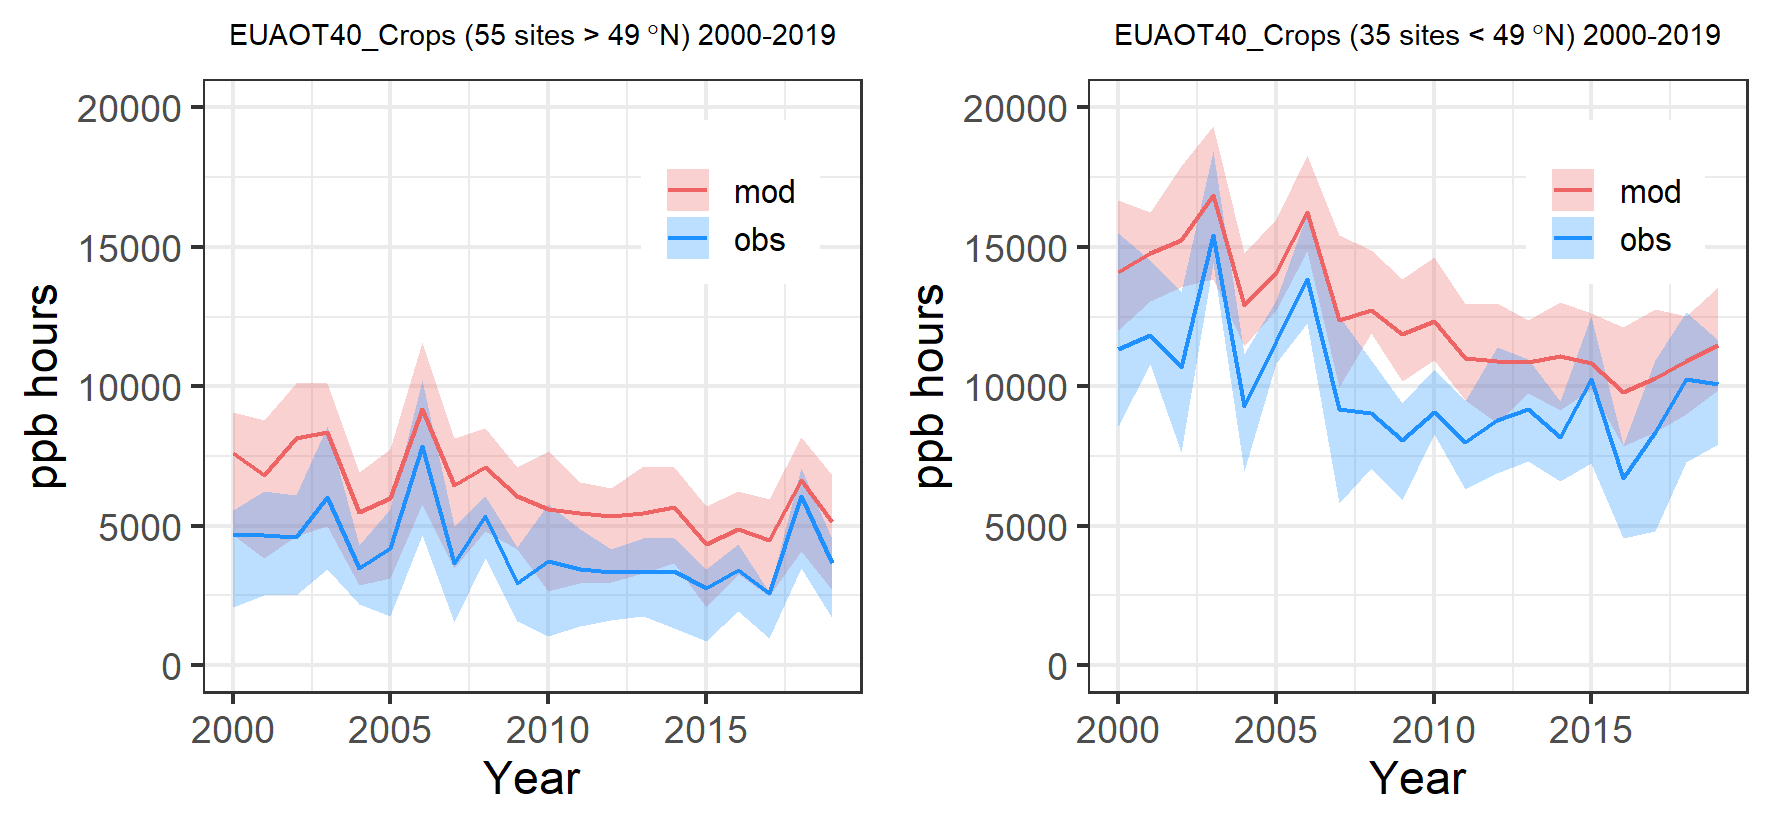
\includegraphics[width=0.74\paperwidth]{FIGS_TRENDS/EUAOT40_Crops_2000_2019_1200m.png}
	\caption{\label{fig:O3_aot40croptrends} Trends in 3-months AOT40 (May-July) for crops from 2000--2019 for EMEP observations and model calculations for sites north (left) and south (right) of 49\degrees N: The solid line indicates the mean, and the shaded area marks the 25th and 75th percentile. Only sites below 1200 m asl and with at least 15 years of data are included.}
\end{figure}

\begin{figure}[h]
	\centering
	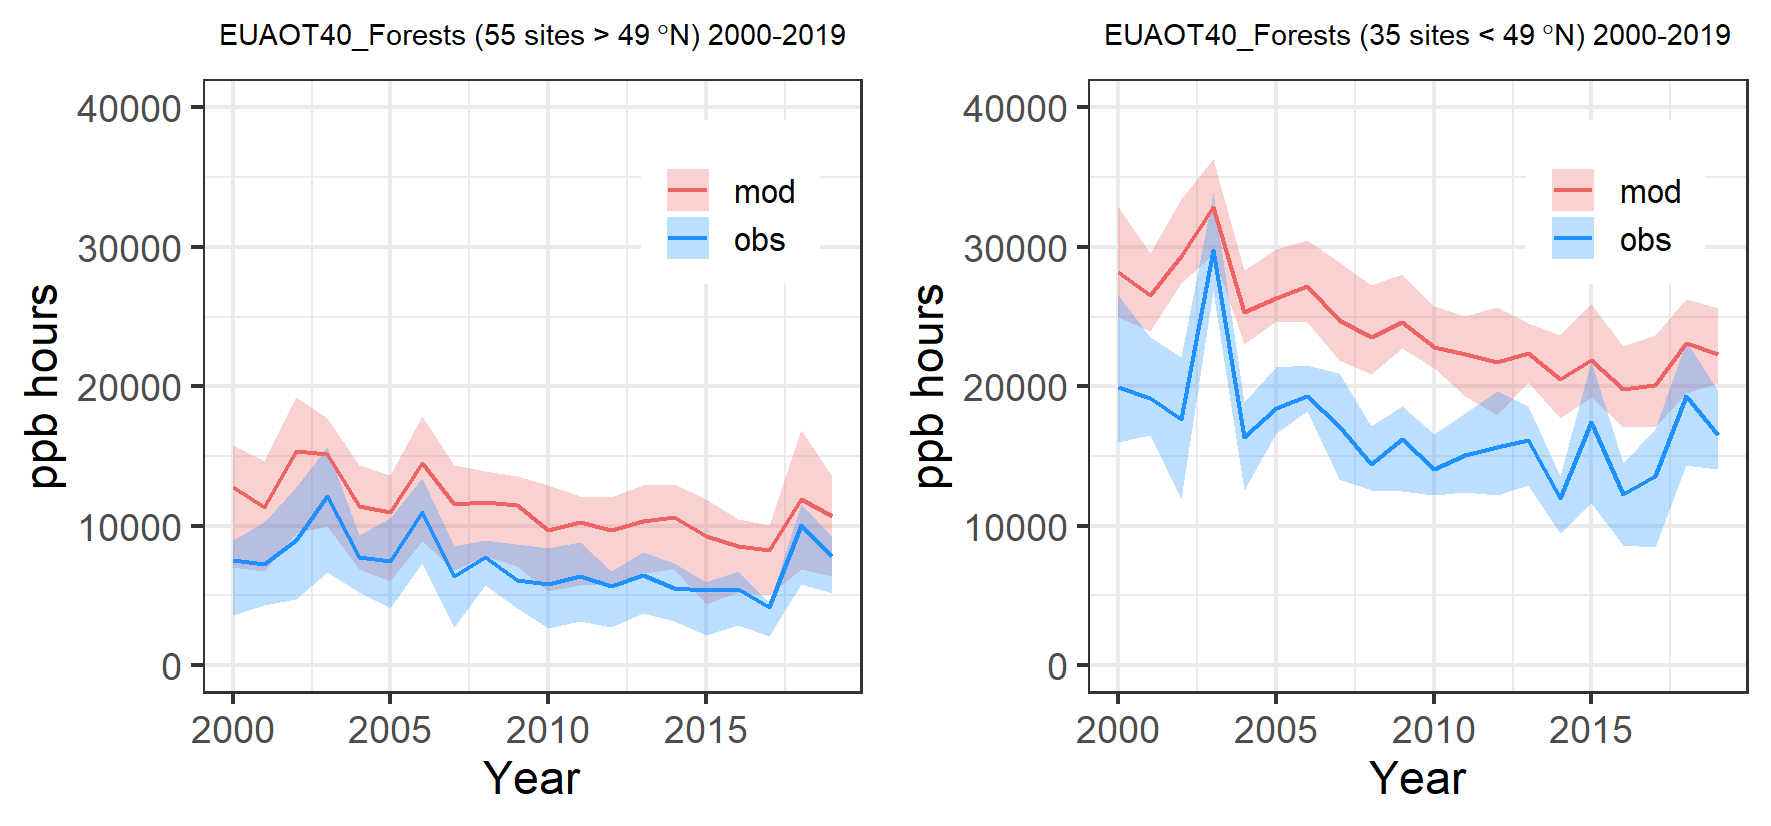
\includegraphics[width=0.74\paperwidth]{FIGS_TRENDS/EUAOT40_Forests_2000_2019_1200m.png}
	\caption{\label{fig:O3_aot40foresttrends}Trends in 6-months AOT40 (Apr-Sep) for forests from 2000--2019 for EMEP observations and model calculations for sites north (left) and south (right) of 49\degrees N: The solid line indicates the mean, and the shaded area marks the 25th and 75th percentile. Only sites below 1200 m asl and with at least 15 years of data are included.}
\end{figure}

\begin{figure}[h]
	\centering
	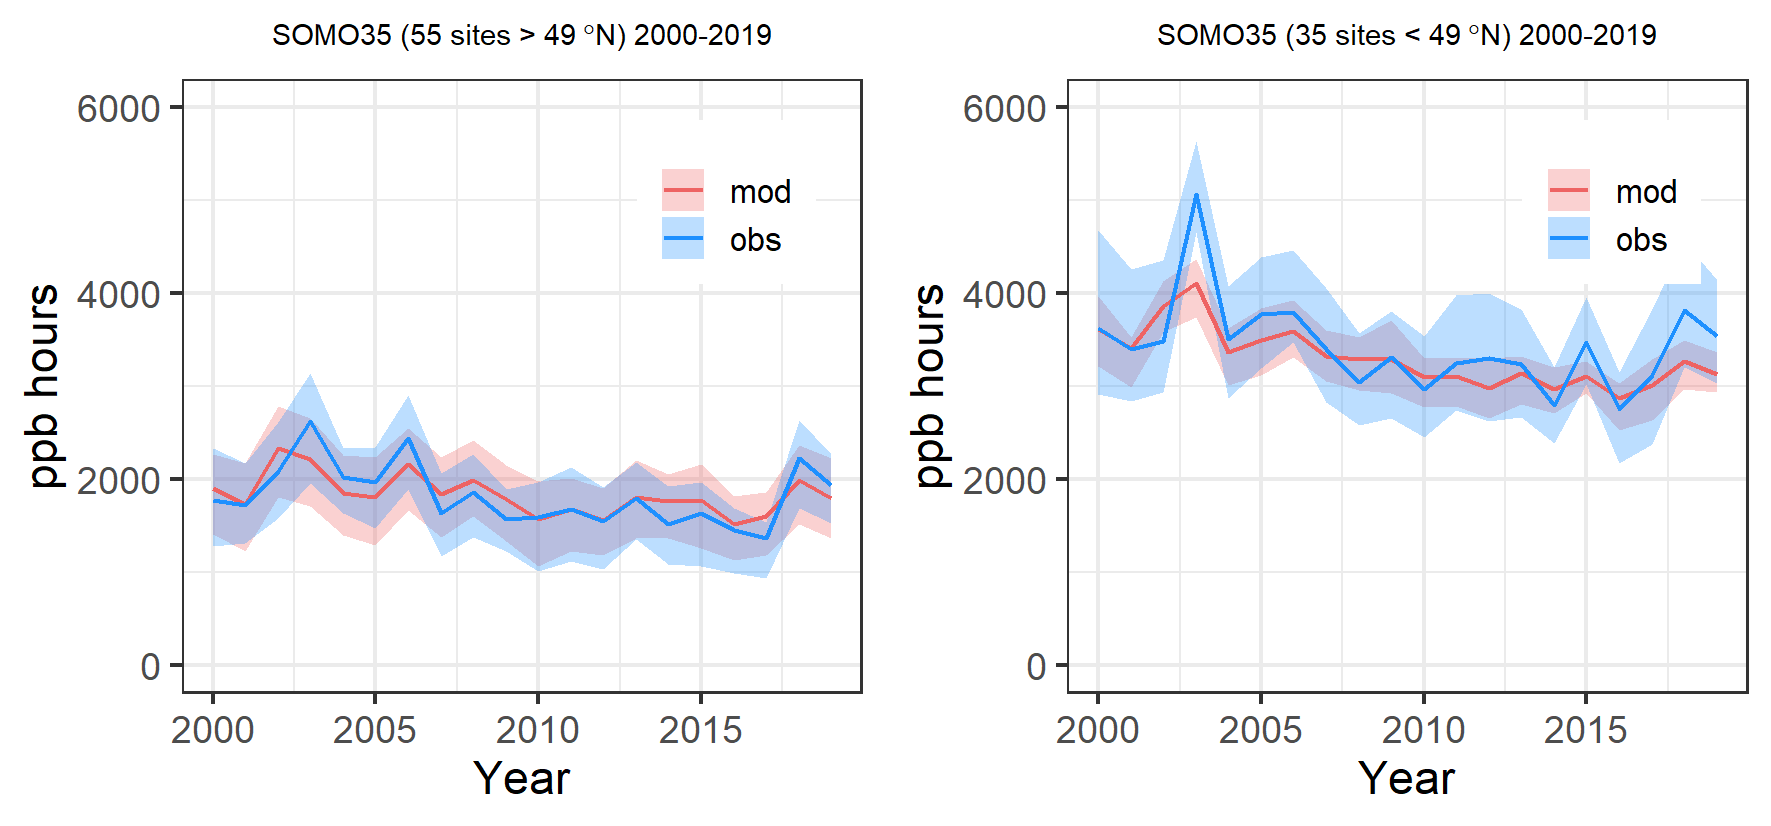
\includegraphics[width=0.74\paperwidth]{FIGS_TRENDS/SOMO35_2000_2019_1200m.png}
	\caption{\label{fig:O3_somo35trends}Trends in SOMO35 from 2000-2019 for EMEP observations and model calculations for sites north (left) and south (right) of 49\degrees N: The solid line indicates the mean, and the shaded area marks the 25th and 75th percentile. Only sites below 1200 m asl and with at least 15 years of data are included.}
\end{figure}


%%%%%%%%%%%%%%%%%%%%%%%%%%%%%%%%%%%%%%%%%%%%%%%%%%%%%%%%%%%%%%%%%%%%%%%%%%%%

\clearpage
\section{Trends in Elemental and Organic Carbon}
\label{sec:trendsECOC}
\subsection{Elemental Carbon, EC}
\label{ss:trendsEC}

Table~\ref{tab:KEX1} presents the absolute and relative changes over 2010-2019 from 15 EMEP sites, as annual values, and with confidence intervals, and from both observed and modelled values. The spatial variation of these trends for summer and winter can be seen as `arrow' plots in Fig.~\ref{fig:ECarrows}, and Fig.\ref{fig:ECtrends} shows again the annual trends, but superimposed upon the field of modelled EC.
Fig.~\ref{fig:KEX1} illustrates the statistics of the reductions in EC over the period 2010--2019, and for different seasons. 

%
Considering first the observed trends in elemental carbon (EC) for 2010--2019, a  reduction (-4.5$\pm$1.5~\%/yr, Tab.~\ref{tab:KEX1}) 
 was
calculated for the 15 sites assessed, which is
quite comparable to the reduction (-5.0$\pm$0.9~\%/yr)
calculated for the eleven sites where the reduction was statistically
significant. The reduction was rather similar considering these eleven
sites, ranging from -4.2~\%/yr to -5.8~\%/yr for ten out of eleven
sites. %, thus we see no apparent spatial pattern in the reductions
The largest reduction was seen amongst the sites with the
highest EC levels, i.e., at Iskrba (-7~\%/yr) in Slovenia and at Ispra
(-5.8~\%/yr) in the Po Valley region in Northern Italy (Fig.~\ref{fig:ECtrends}). Notably, these
were the only sites where a statistically significant reduction was
observed for all seasons, being most pronounced in summer, although
by a small margin. When considering all sites, the reduction was most
pronounced in summer and fall (Tab.~\ref{tab:KEX1},Fig.~\ref{fig:KEX1}), but the general picture is
that there is a minor seasonal variability in the reduction of EC. It can be noted though that
there are more sites with significant trends (p-values $<$ 0.05)  in summer than winter (Fig.\ref{fig:ECarrows}).

Fig.~\ref{fig:KEX1} illustrates the statistics of the reductions in EC  n both observed and model results over the period 2010-2019, and for different seasons. For EC, the model is seen to capture the year to year changes very well over the ten years, and captures well the relative changes which are ca. -4~\%/yr in all seasons. Larger differences are seen in the absolute changes (which may reflect the difficulties with the EC emissions mentioned in Sect.~\ref{ss:IssuesECOC}).
These points about model-measurement comparison for EC are discussed further in Sect.~\ref{ss:DiscECOC}.

\begin{table}
 \caption{Absolute change (\ugC/yr) and relative change (\%/yr) and
  corresponding confidence intervals in observed and modelled annual
  and seasonal aggregated EC concentrations at 15 sites across Europe
  for 2010--2019. The number of sites with a significant outcome is
  provided. \label{tab:KEX1}}
% \begin{tabular}{lrrrrlrlrlrl}
%\begin{center}
\scalebox{0.65}{%
\begin{tabular}{llcc|cccc|cccc}
\toprule
%\hline
               \multicolumn{4}{c}{Number of sites} & \multicolumn{4}{c}{Absolute change (\ug $yr^{-1})$} & \multicolumn{4}{c}{Relative change (\% $yr^{-1}$)} \\
 Season &           Total & Sign. & Sign. &                   obs. &          Conf.interval &  Mod. &          Conf.interval &                     Obs. &         Conf.interval &  Mod. &        Conf.interval \\
       &                  & (Obs.)    & (Mod.)     &   &  &  & & & & & \\
\midrule
%\hline
All    &              15 &         11 &          12 &                  -0.019 &  (-0.031, -0.008) & -0.014 &  (-0.021, -0.007) &                    -4.49 &  (-5.25, -3.73) & -3.81 &  (-4.59, -3.03) \\
Winter &              15 &          6 &           4 &                  -0.029 &  (-0.053, -0.006) & -0.019 &  (-0.032, -0.006) &                    -4.27 &  (-5.49, -3.06) & -3.10 &  (-4.21, -1.98) \\
Spring &              15 &          5 &           8 &                  -0.012 &  (-0.018, -0.006) & -0.013 &  (-0.018, -0.009) &                    -3.88 &  (-4.67, -3.09) & -3.86 &   (-4.92, -2.8) \\
Summer &              15 &          8 &          10 &                  -0.011 &  (-0.015, -0.007) & -0.008 &  (-0.013, -0.004) &                    -4.73 &  (-5.71, -3.74) & -3.71 &  (-4.59,  -2.82) \\
Autumn &              15 &          8 &          11 &                  -0.023 &   (-0.036, -0.01) & -0.018 &  (-0.027, -0.009) &                    -4.96 &   (-6.03, -3.9) & -4.25 &  (-5.15,  -3.35) \\
\bottomrule
\end{tabular}
} % end scalebox
\end{table}

%%%%%%%%%%%%%%%%%%%%%%%%%%%%%%%%%%%%%%%%%%%%%%%%%
% trim L L R U 
\begin{figure}
\includegraphics*[height=6cm,trim=3cm 0 0 0]{FIGS_TRENDS/Plot_ec_rel_summer_Model.png}%
\includegraphics*[height=6cm,trim=3cm 0 6.5cm 0]{FIGS_TRENDS/Plot_ec_rel_summer_Observations.png}
\\
\includegraphics*[height=6cm,trim=3cm 0 0 0]{FIGS_TRENDS/Plot_ec_rel_winter_Model.png}%
\includegraphics*[height=6cm,trim=3cm 0 6.5cm 0]{FIGS_TRENDS/Plot_ec_rel_winter_Observations.png}
\caption{Relative trends for EC in \pmfine over the period of 2010-2019, from both model (left) and observations (right), and for summer (top) and winter (bottom). The magnitude of the trends is indicated by the angle made (see key), which also indicates the trend values associated with 45\degrees and 90\degrees angles. The colour indicates the p-values associated with the trends. (The style of these plots is based upon those used in the ROAR project, e.g.\citealt{MillsTOAR:2018}.) 
  \label{fig:ECarrows}}
\end{figure}
%%%%%%%%%%%%%%%%%%%%%%%%%%%%%%%%%%%%%%%%%%%%%%%%%
%%%%%%%%%%%%%%%%%%%%%%%%%%%%%%%%%%%%%%%%%%%%%%%%%%%%%%
\begin{figure}  %DS[H]
  \centering{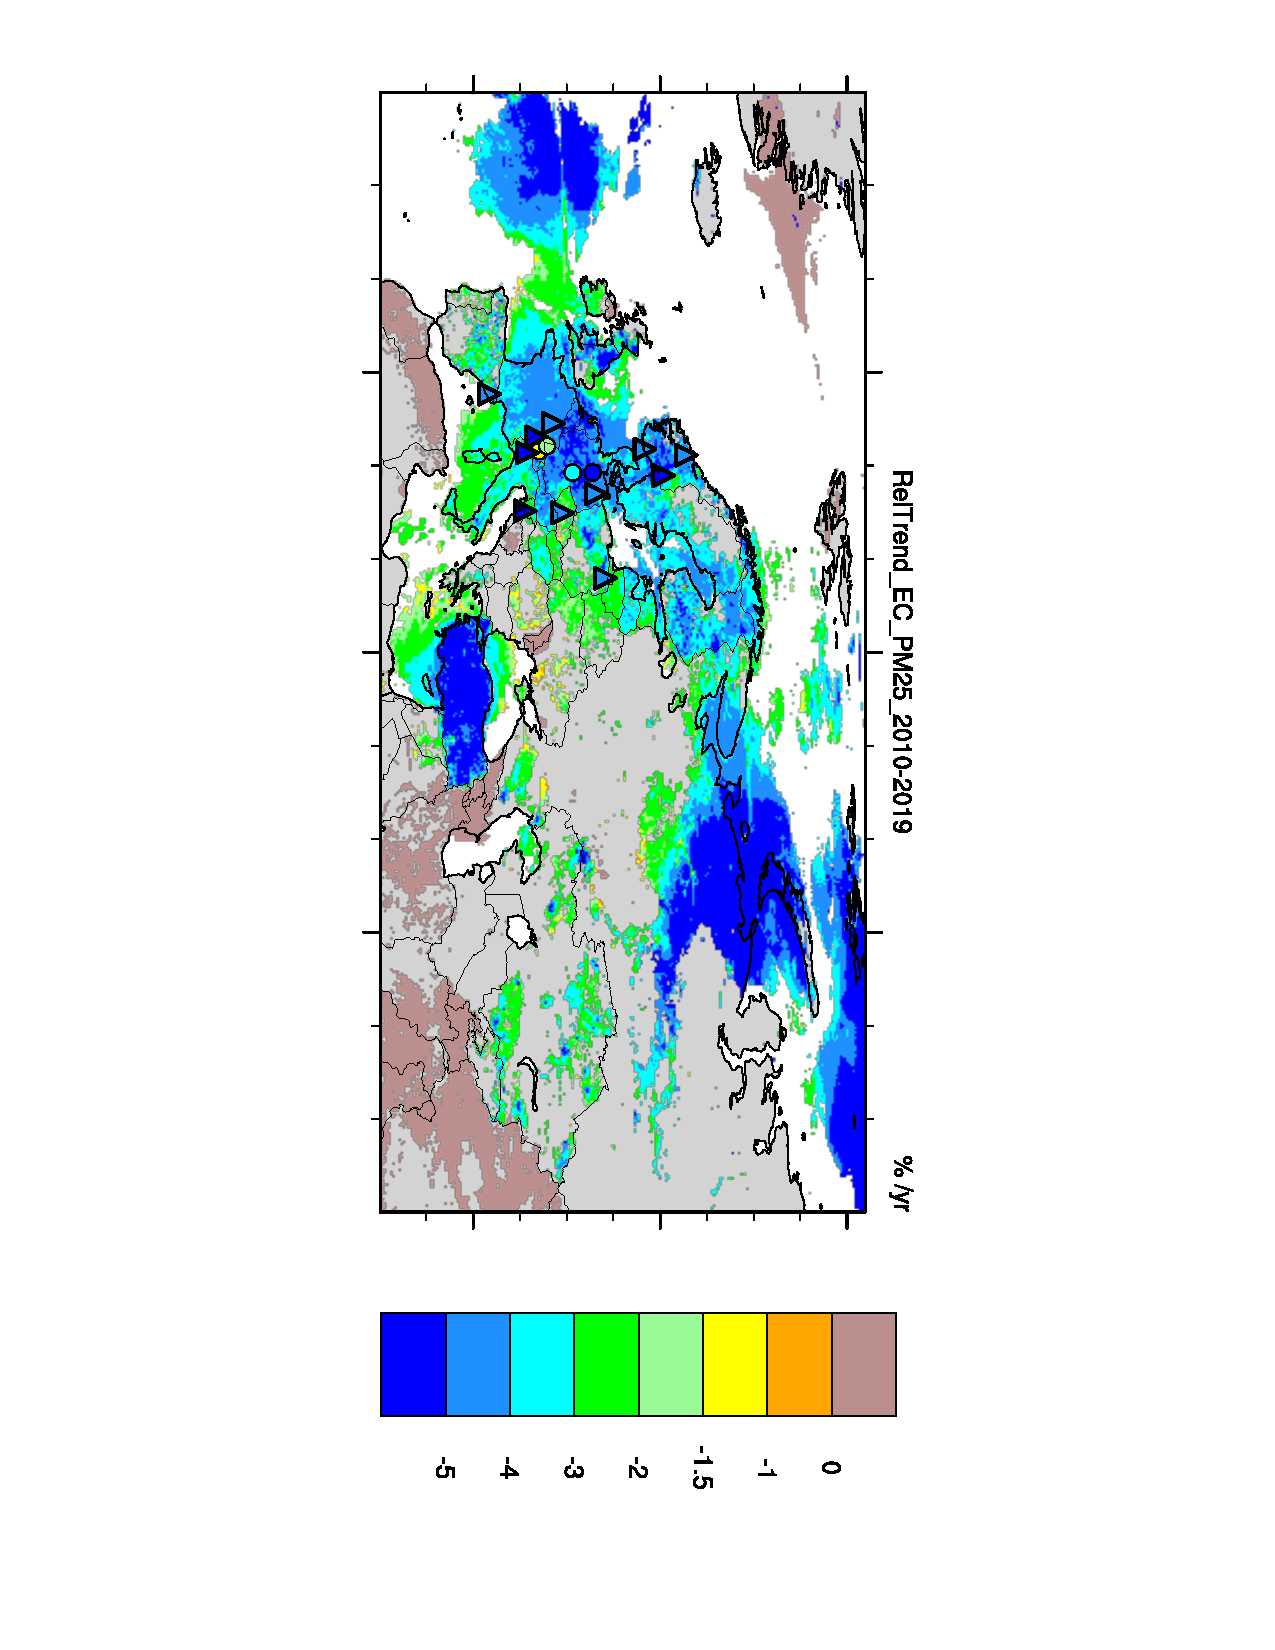
\includegraphics[clip=,angle=90,height=6.1cm,viewport=175 67 448 754]{FIGS_TRENDS/RelTrend_EC_PM25_2010-2019_Perc.pdf}}\\
%  \vspace{0.5cm}
%  \centering{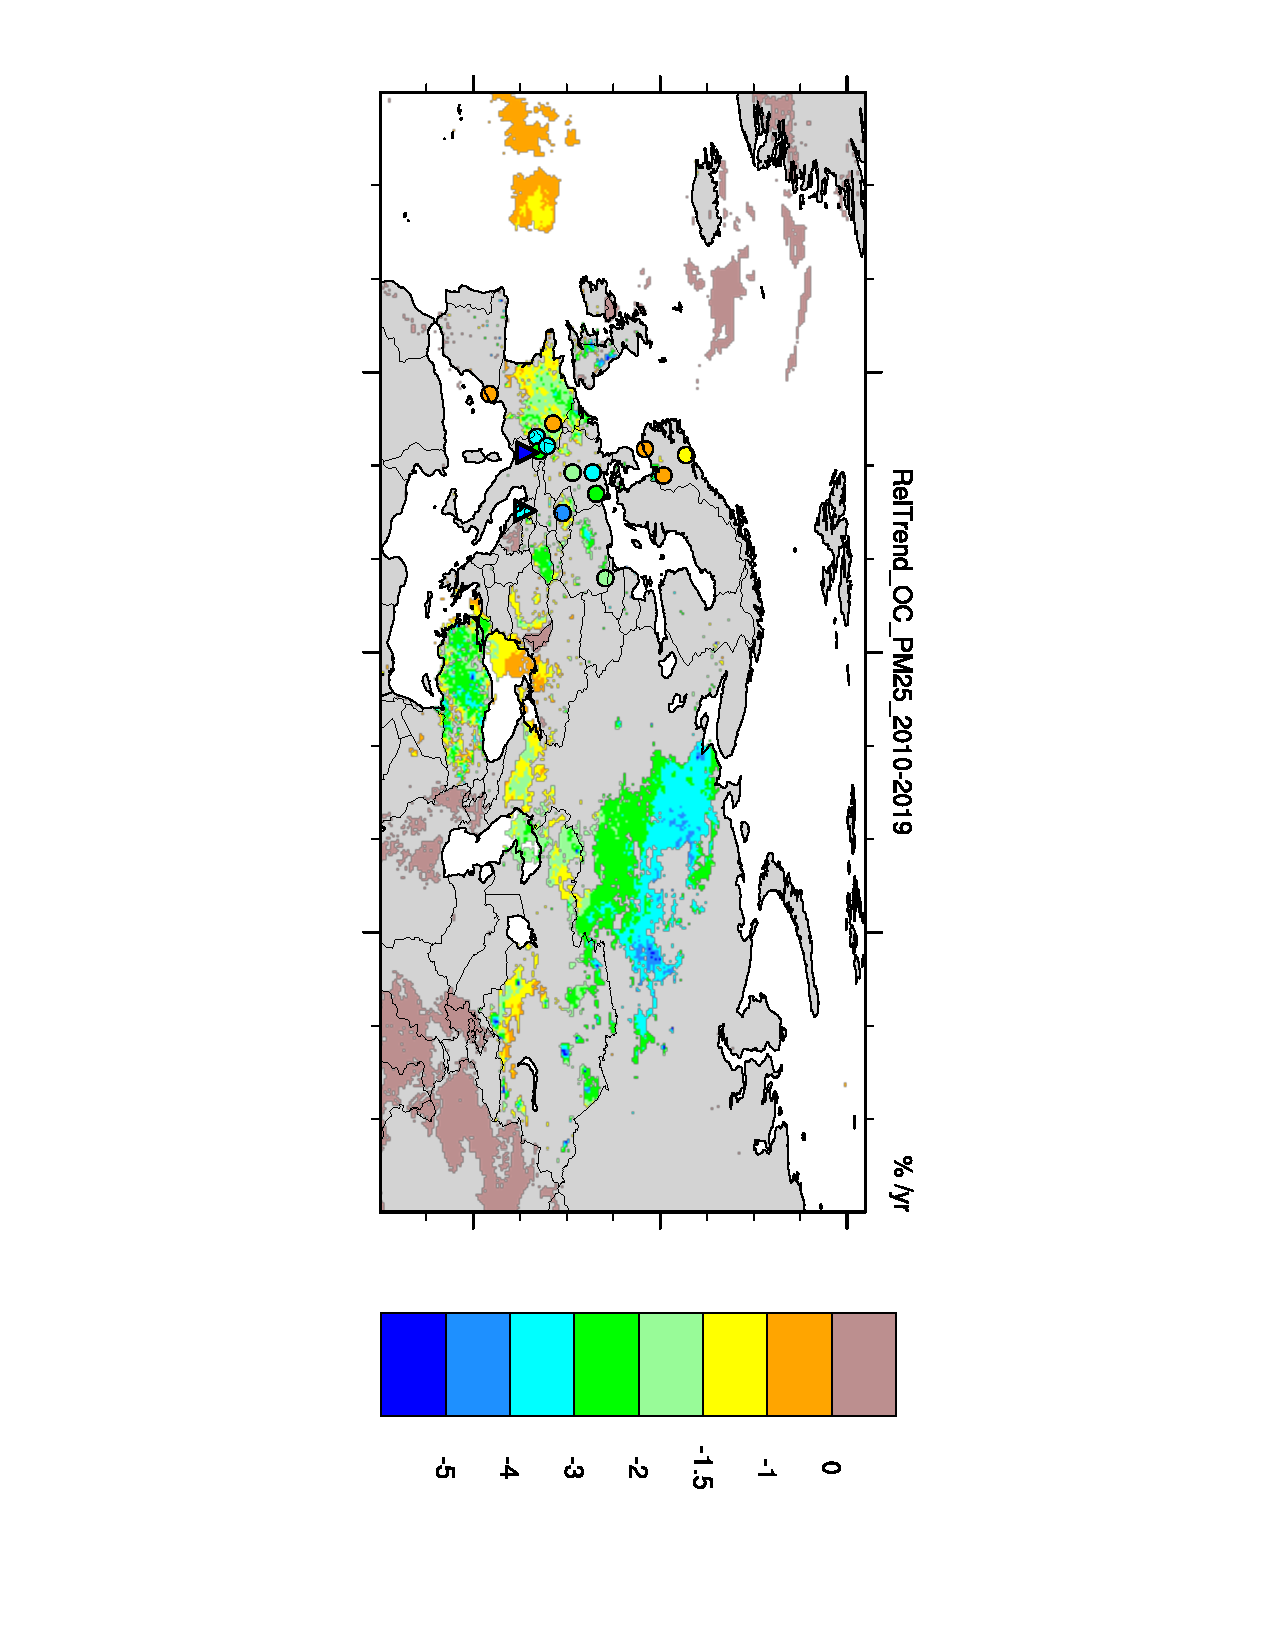
\includegraphics[clip=,angle=90,height=6.1cm,viewport=175 67 448 754]{FIGS_TRENDS/RelTrend_OC_PM25_2010-2019_Perc.pdf}}
\caption{Relative trends for EC in \pmfine over the period of 2010--2019: EMEP modelled -- coloured contours (grey/white means non-significant trends) and observed - coloured triangles (significant) and circles (non-significant).}
\label{fig:ECtrends}
\end{figure}
%%%%%%%%%%%%%%%%%%%%%%%%%%%%%%%%%%%%%%%%%%%%%%%%%


\begin{figure}[t]
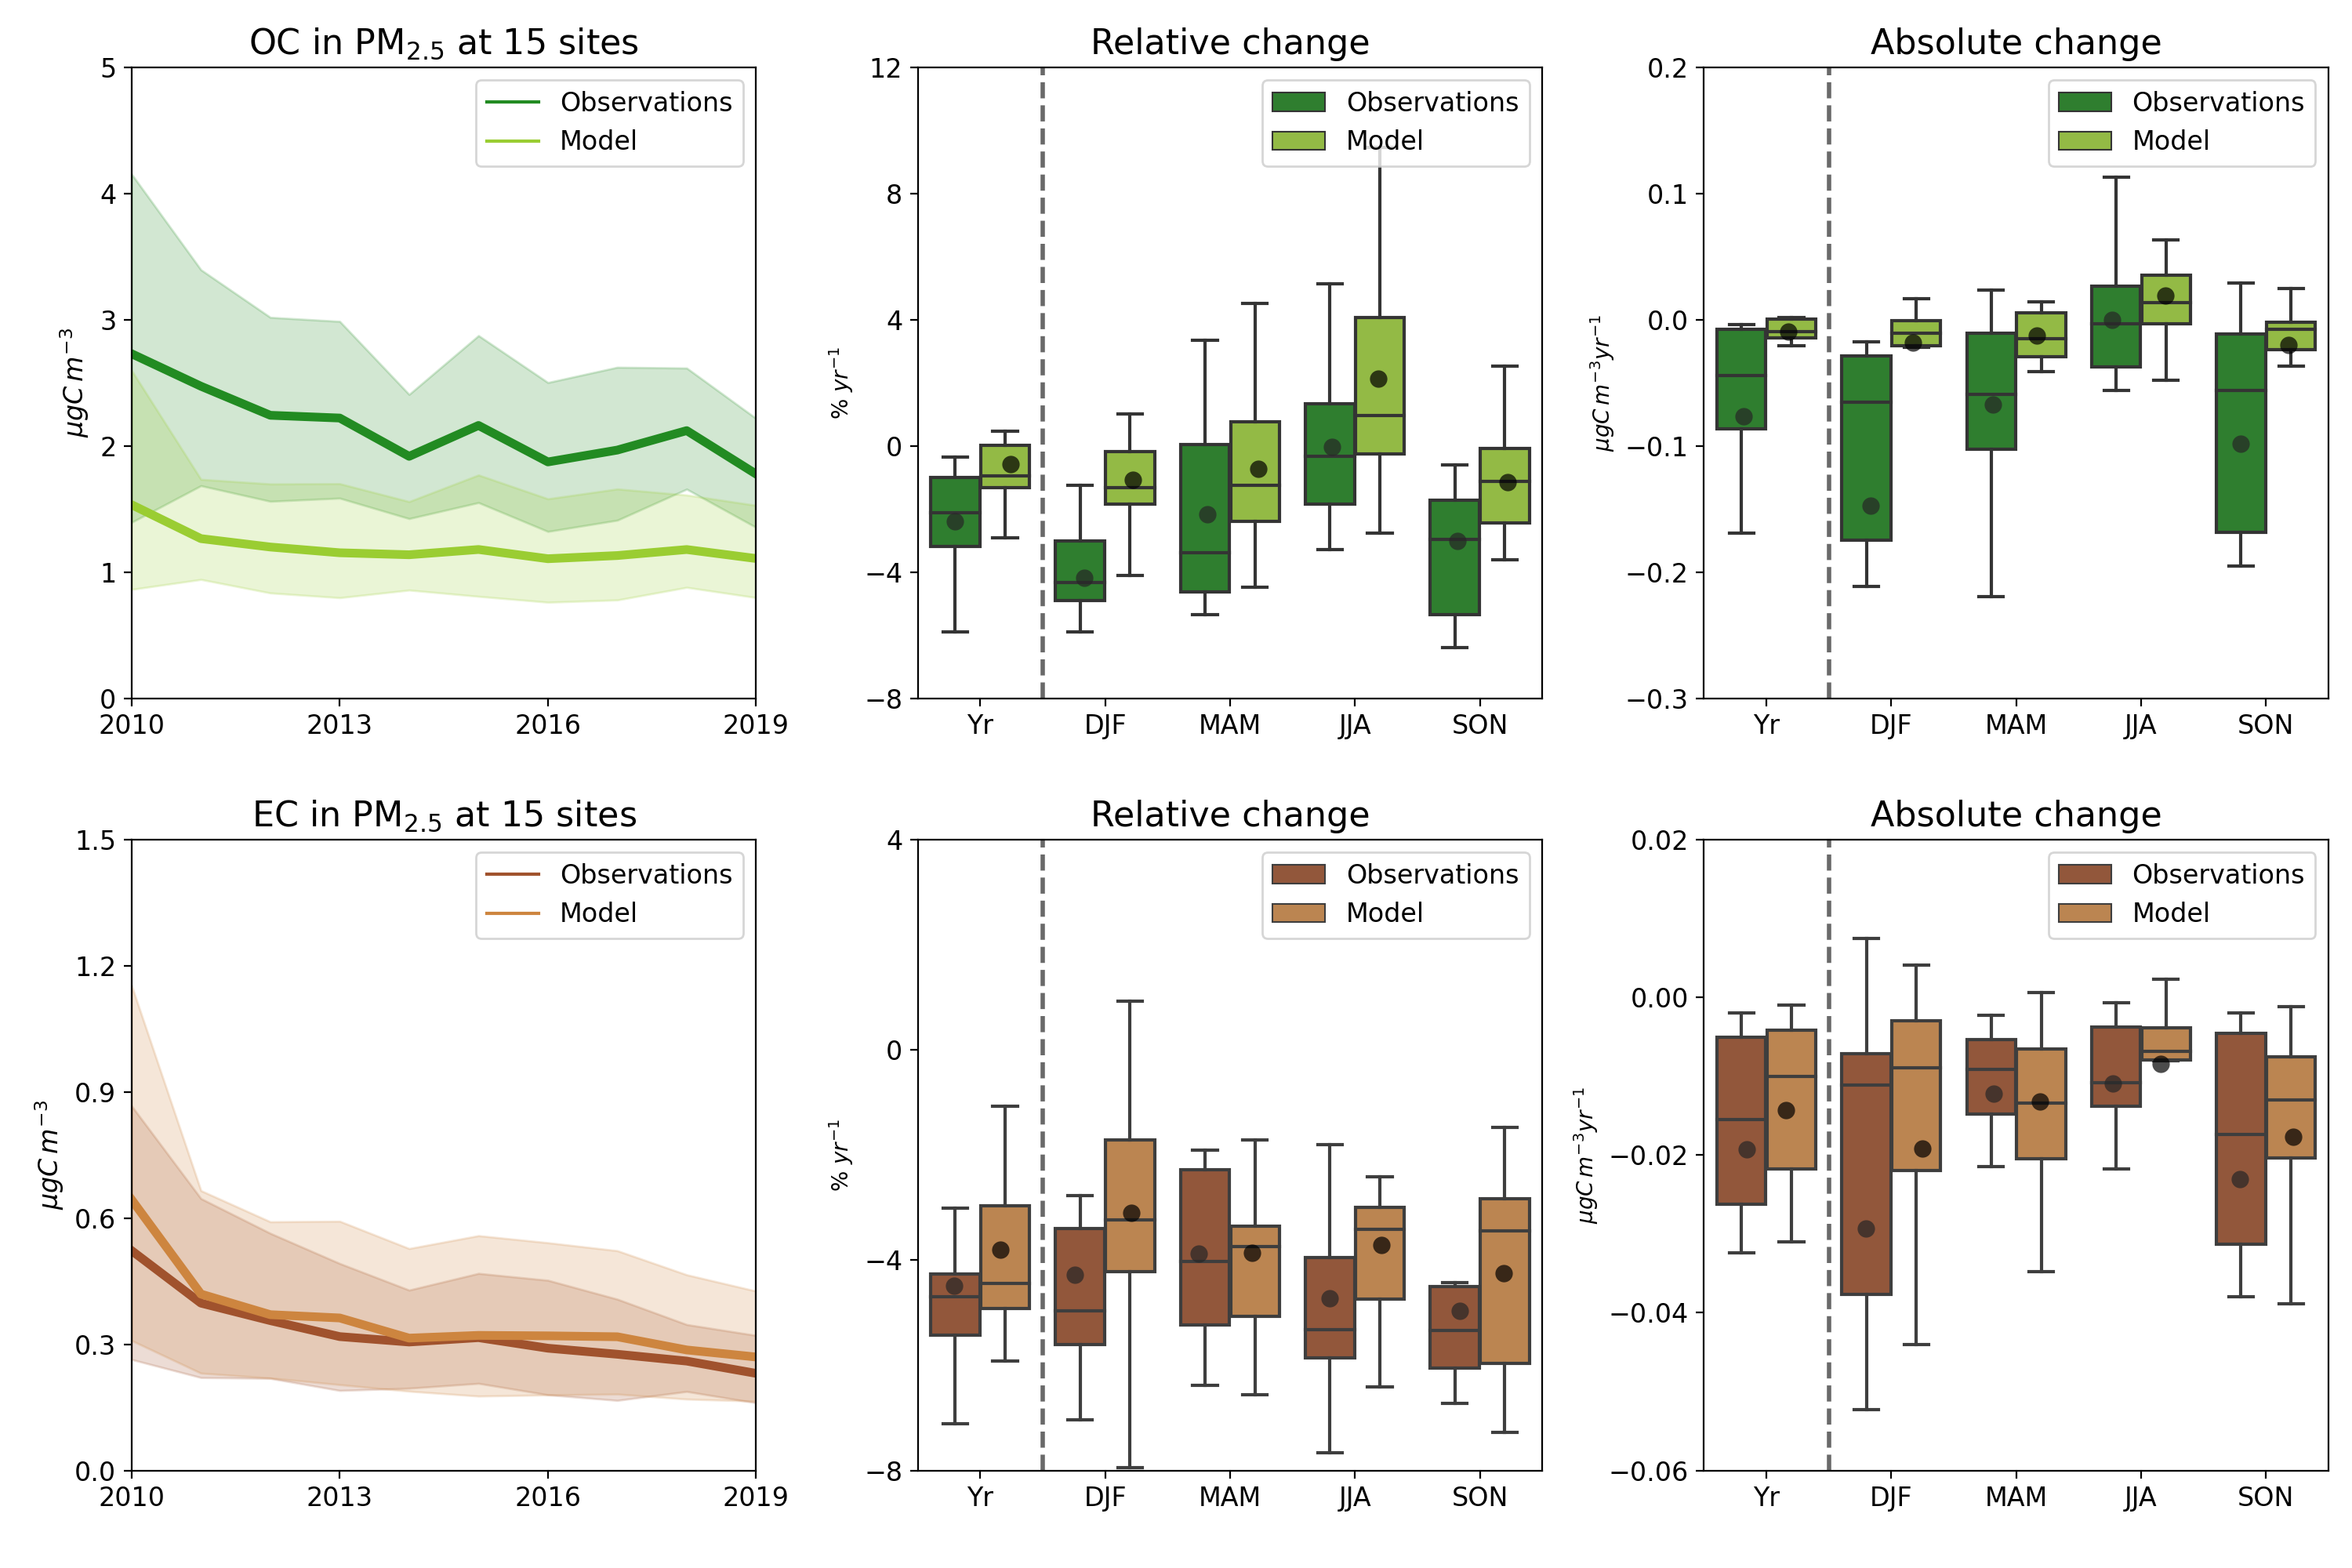
\includegraphics[width=16cm]{FIGS_TRENDS/ECOC_trends.png}
\caption{Observed and modelled concentrations and trends of EC and OC at 15 EMEP
  site across Europe for 2010--2019, showing the concentrations
  (left panels) of OC (upper) and EC (lower), aggregated annual and
  seasonal relative changes (mid panels) for OC (upper) and EC (lower),
  and aggregated annual and seasonal absolute changes (right panels)
  for OC (upper) and EC (lower). The solid line in the left panel shows
  the average annual mean for all sites and the shaded area the 95\%
  confidence interval. The box plots in the mid and right panels show
  the 25th and 75th percentiles (boxes), the median (horizontal lines),
  whereas the whiskers represent the interquartile ranges $\times$
  1.5 and the squares the outliers. Black markers within the box are
  the means.\label{fig:KEX1}
}
\end{figure}







\subsection{Organic Carbon, OC}
\label{ss:trendsOC}
 
 Table~\ref{tab:KEX2} presents the absolute and relative changes in OC over 2010-2019 from 15 EMEP sites, as annual values and with confidence intervals, and from both observed and modelled values. The spatial variation of these trends for summer and winter can be seen as `arrow' plots in Fig.~\ref{fig:OCarrows}, and Fig.\ref{fig:OCtrends} shows again the annual trends, but superimposed upon the modelled field of modelled OC.
Fig.~\ref{fig:KEX1} illustrates the statistics of the reductions in OC  over the period 2010-2019, and for different seasons. 
 %
A 2.4$\pm$1.6~\%/yr reduction
  in organic carbon (OC) for 2010--2019
was calculated for the 15 sites assessed (Tab.~\ref{tab:KEX2}), but the
downward trend was statistically significant only for Iskrba (Slovenia)
and Ispra (Italy), which are amongst the sites with the highest OC
loading. At these two sites, the reduction was noticeably higher 
(-3.1~\%/yr at Iskrba, -5.9~\%/yr at Ispra) than for the mean of all sites. The
reduction in OC appears somewhat lower at the westernmost and northernmost
sites (Fig.\ref{fig:OCtrends}). 




There was a pronounced seasonal variability in the reduction observed for
OC (Tab.~\ref{tab:KEX2}, Figs.~\ref{fig:KEX1},\ref{fig:OCarrows}). In winter, the
 reduction (-4.2~\%/yr) was equal to that for
EC (-4.3~\%/yr, but only statistically significant for six of the sites,
whereas no reduction (0~\%/yr) was seen in summer. Spring (-2.2~\%/yr, Tab.~\ref{tab:KEX2}) and fall (-3.0~\%/yr) are transition seasons with reductions in between
that of winter and summer and statistically significant reductions were
observed only for Ispra. 
%
Figure~\ref{fig:OCarrows} makes it clear that there were large differences in both sign and magnitude of the summertime trends in OC at individual sites, in both modelled and observed results. For the winter trends, Fig.~\ref{fig:OCarrows} shows that essentially all observed wintertime trends were reductions, whereas the modelled trends were more variable and less significant. In summertime the trends can be positive or negative, and are generally not significant.


Fig.~\ref{fig:KEX1} illustrates the statistics of the reductions in OC  over the period 2010-2019, and for different seasons. For OC the model substantially underpredicts the yearly concentrations over the whole period (see also Tab.~\ref{tab:KEX2}), and also underpredicts the trends. There is substantial seasonal variation though. Observed reductions in winter (DJF) of -4.2~\%/yr (Tab.~\ref{tab:KEX2}) are not reproduced by the model at all (-1.1~\%/yr), though even in winter the observed trends were only significant for six of the 15 sites. In summer the observed trends are very small but negative (-0.03~\%/yr), whereas the model suggests positive trends of 2.1~\%/yr. As noted above (c.f. Fig.~\ref{fig:OCarrows}), the summer trends are very different for individual sites, even with respect to the sign of the change, and one cannot assign much significance to the changes. Model-measurement comparison for OC are discussed further in Sect.~\ref{ss:DiscECOC}.

\SKIP{
The model calculated a
reduction in OC of -0.6~\%/yr considering all sites, which was noticeably
less than for the observations (-2.4~\%/yr) (c.f. Tab.~\ref{tab:KEX2}). The model also underpredicted
the decrease calculated for the observations for each season, thereby
reproducing the seasonality in trend seen for the observations. A decrease
in observed OC was calculated for all sites, whereas the model calculated
an increase, typically <0.5~\%/yr, for four of the sites. 
} % END SKIP




%%%%%%%%%%%%%%%%%%%%%%%%%%%%%%%%%%%%%%%%%%%%%%%%%

\begin{table}
 \caption{Absolute change ( \ugC/yr) and relative change (\%/yr) and
   corresponding confidence intervals in observed and modelled annual
   and seasonal aggregated OC concentrations at 15 sites across Europe
   for 2010--2019. The number of sites with a significant outcome
   is provided. \label{tab:KEX2}
 }
 
%\begin{center}
\scalebox{0.7}{%
\begin{tabular}{llcc|cccc|cccc}
\toprule
\multicolumn{4}{c}{Number of sites} & \multicolumn{4}{c}{Absolute change (\ug $yr^{-1})$} & \multicolumn{4}{c}{Relative change (\% $yr^{-1}$)} \\
Seasons &  No. & sign. & sign. &                    obs. &          conf.interval &  mod. &          conf.interval &                     obs. &         conf.interval &  mod. &        conf.interval \\
       &                 &  (obs.)    & (mod.)  & & & & & & & & \\
\midrule
all    &              15 &          2 &           1 &                  -0.077 &  (-0.132, -0.022) & -0.009 &     (-0.019, 0.0) &                    -2.40 &  (-3.23, -1.57) & -0.59 &   (-1.21, 0.03) \\
winter &              15 &          6 &           1 &                  -0.148 &  (-0.249, -0.047) & -0.018 &  (-0.032, -0.004) &                    -4.19 &  (-5.16, -3.22) & -1.09 &  (-2.03, -0.15) \\
spring &              15 &          1 &           0 &                  -0.067 &   (-0.104, -0.03) & -0.013 &  (-0.023, -0.003) &                    -2.18 &  (-3.68, -0.67) & -0.74 &   (-1.94, 0.47) \\
summer &              15 &          0 &           1 &                  -0.000 &   (-0.024, 0.023) &  0.019 &   (-0.003, 0.041) &                    -0.03 &   (-1.19, 1.12) &  2.13 &    (0.44, 3.83) \\
autumn &              15 &          1 &           0 &                  -0.098 &   (-0.16, -0.037) & -0.020 &     (-0.041, 0.0) &                    -3.03 &  (-4.43, -1.62) & -1.16 &   (-2.47, 0.15) \\
\bottomrule
\end{tabular}
} % end scalebox
\end{table}




%%%%%%%%%%%%%%%%%%%%%%%%%%%%%%%%%%%%%%%%%%%%%%%%%

\begin{figure}
\includegraphics*[height=6cm,trim=3cm 0 0 0 0]{FIGS_TRENDS/Plot_oc_rel_summer_Model.png}%
\includegraphics*[height=6cm,trim=3cm 0 6.9cm 0]{FIGS_TRENDS/Plot_oc_rel_summer_Observations.png}
\\
\includegraphics*[height=6cm,trim=3cm 0 0 0]{FIGS_TRENDS/Plot_oc_rel_winter_Model.png}%
\includegraphics*[height=6cm,trim=3cm 0 6.9cm 0]{FIGS_TRENDS/Plot_oc_rel_winter_Observations.png}
\caption{Relative trends for OC in \pmfine over the period of 2010-2019, from both model (left) and observations (right), and for summer (top) and winter (bottom). (See Fig.~\ref{fig:ECarrows} for further details.)
 \label{fig:OCarrows}}
\end{figure}

%%%%%%%%%%%%%%%%%%%%%%%%%%%%%%%%%%%%%%%%%%%%%%%%%%%%%%
\begin{figure}  %DS[H]
%  \centering{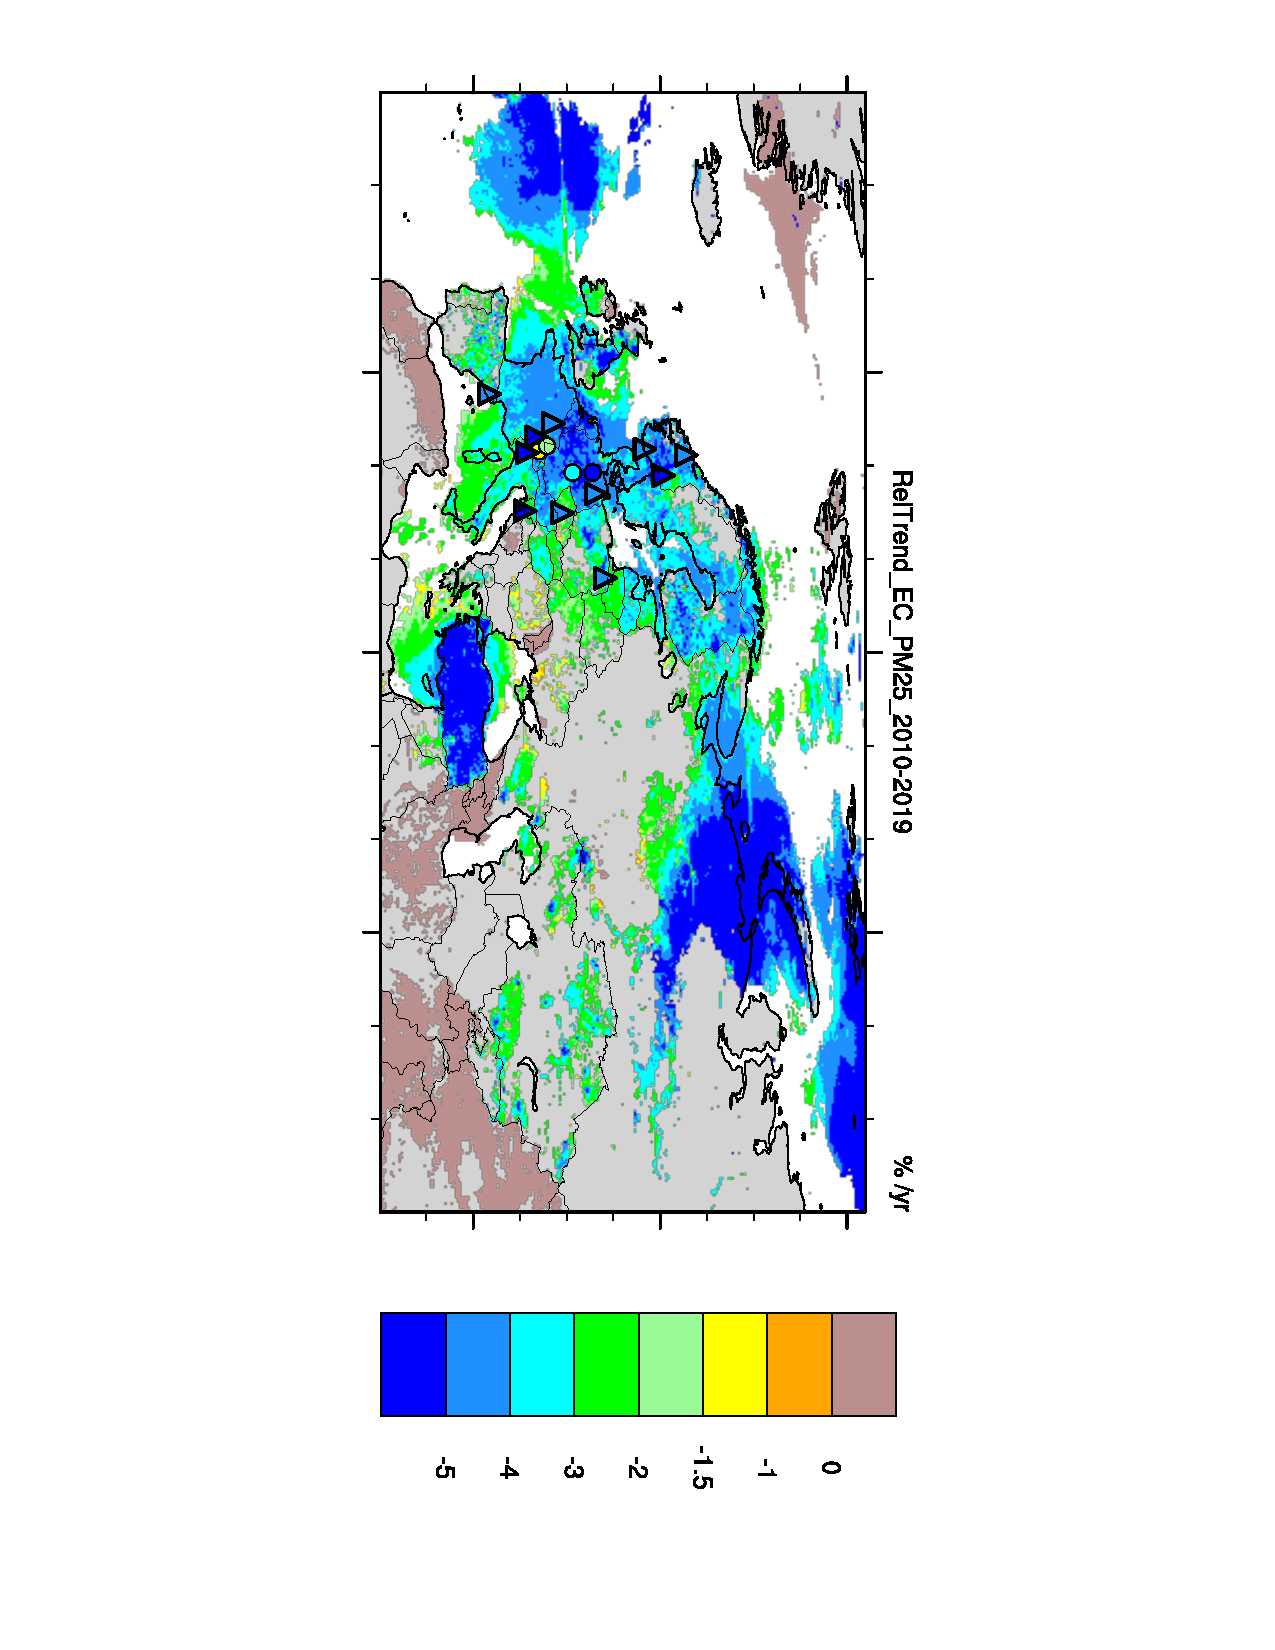
\includegraphics[clip=,angle=90,height=6.1cm,viewport=175 67 448 754]{FIGS_TRENDS/RelTrend_EC_PM25_2010-2019_Perc.pdf}}\\
%  \vspace{0.5cm}
\centering{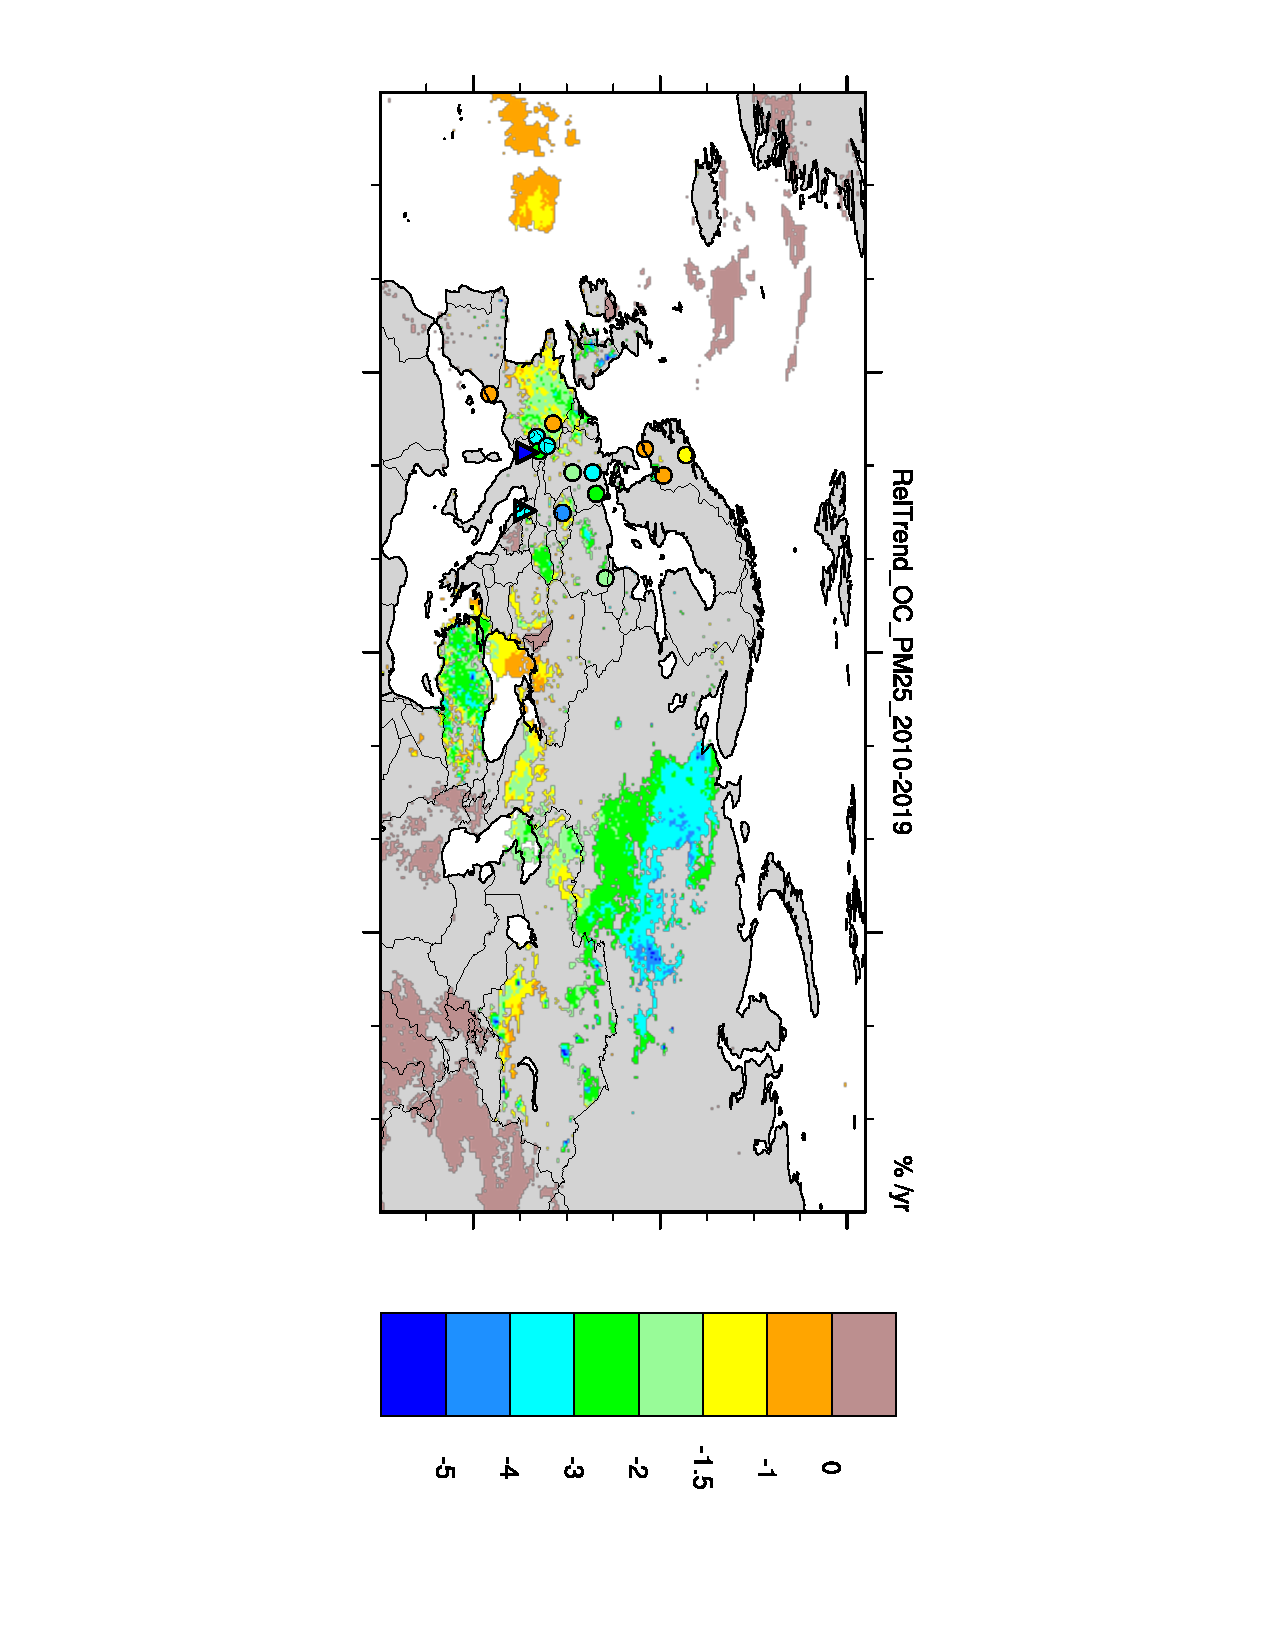
\includegraphics[clip=,angle=90,height=6.1cm,viewport=175 67 448 754]{FIGS_TRENDS/RelTrend_OC_PM25_2010-2019_Perc.pdf}}
\caption{Relative trends for OC in \pmfine over the period of 2010-2019: EMEP modelled -- coloured contours (grey/white means non-significant trends) and observed - coloured triangles (significant) and circles (non-significant).}
\label{fig:OCtrends}
\end{figure}
%%%%%%%%%%%%%%%%%%%%%%%%%%%%%%%%%%%%%%%%%%%%%%%%%

\subsection{Discussion of EC, OC trends}
\label{ss:DiscECOC}

Before discussing the trends shown in Sect.~\ref{ss:trendsEC}-\ref{ss:trendsOC} in  more detail, it is important to note that ten years is a short period over which to assess such trends. In order to illustrate this, Table~\ref{tab:BirkenesTrends} shows trends assessed for three periods, 2008-2018, 2008-2019, and 2010-2019, all using the same methodology. It is seen that the magnitude of the trends can differ substantially depending on the time-window. For EC the values range from -2.2~\%/yr to \mbox{-4.2~\%/yr}, and for levoglucosan from -2.5~\%/yr to -5.2~\%/yr, with all values satisfying the p-value$<$0.05 significance test. Trend values for OC vary even more, but these trends were insignificant for all periods. Although we expect some of these trends to reflect changes in emissions, meteorological variation will also play a large role, especially in causing the high sensitivity of the calculated trends to small changes in the time window chosen.


\begin{table}[H]
\centering
\parbox{11.9cm}{
\caption{Relative trends (\%/yr) (and p-values in parentheses) calculated for Birkenes 
    using different time-windows \label{tab:BirkenesTrends}}}
\begin{tabular}{lcccc}
\toprule
     &         & 2008-2018$^{(a)}$& 2008-2019     & 2010-2019       \\
\midrule
 & & & & \\
%\multicolumn{5}{c}{Revised from Wenche 26/8/21} \\
EC   & annual  & -3.0 (0.043)        &  -2.21 (0.034)   & -4.24 (0.012) \\
OC   & annual  &  -0.44 (0.876)      &   0.18 (--)$^{(b)}$     & -0.64 (--)   \\
Levoglucosan & annual  & -2.5 (0.043)        &  -2.48 (0.024)   & -5.2  (0.032) \\
& & & & \\
\bottomrule 
\end{tabular}\\
\parbox{11.9cm}{

Notes:
(a) Values for 2008-2018 use same procedure as for 2008-2019 and 2010-2019.
Due to minor screening differences, numbers
differ slightly from results of \citet{Yttri2021}, which had 2008-2018 trends of -4.2~\%/yr for EC and -2.8~\%/yr for levoglucosan;
(b) dash (--) indicates highly insignificant p-value.\\
}
\end{table}


The 2010-2019 reduction of 4.2~\%/yr in observed EC across all seasons is rather dramatic, though as noted above a different choice of time-window might suggest a lower magnitude of changes. 
As discussed in Sect.~\ref{ss:trendsEC} there is only a minor seasonal variability in the reduction of EC. This partly reflects the minor seasonal variability in most EC sources, but it is puzzling since residential heating (in GNFR sector C) should have clear winter maxima. \citet{Yttri2021} found that the reduction in EC
was most pronounced in spring and summer at the Birkenes Observatory in
southern Norway for 2001--2018, arguing that this was due to influence
from less abated sources such as domestic heating in winter and fall. This argument was
supported by a smaller change (-2.8~\%/yr) for the biomass burning
tracer levoglucosan (2008--2018) than for EC (-4.2~\%/yr) (these trend numbers are from \citeauthor{Yttri2021}, and differ slightly from trends calculated for this report, c.f. Tab.~\ref{tab:BirkenesTrends}). In this study, however, 
we calculated a -5.2~\%/yr change (i.e. reduction) for the biomass burning tracer
levoglucosan observed at the Birkenes Observatory for 2010-2019, which is
greater than the -4.2~\%/yr change calculated for EC.
%, which might suggest that abatement of carbonaceous aerosol from biomass burning has been equally successful as that of EC from fossil fuel sources. This 
This finding seems to contradict the conclusion made
by \citet{Yttri2021}, but the differences in trends using different time-windows (c.f.Tab.~\ref{tab:BirkenesTrends}) suggests it is difficult to draw firm conclusions about these changes.


As the biomass burning emissions observed at the
Birkenes Observatory is largely long-range transported from Continental
Europe and Western Russia \citep{Yttri2021}, our findings for Birkenes
are likely to be representative for a larger part of Europe. However,
changing footprints  for the Birkenes site may also affect both the trends and
the relative contributions of biomass burning and residential wood combustion (RWC).
Figure~\ref{fig:gnfrCtrends} shows that for some countries, for example France, GNFR C \pmfine emissions have been in constant decline throughout the 2000s. Declines are seen in other countries from around 2010 onwards also, and most of these (arnitrailty chosen) countries show reduction of ca.~4~\%/yr. Thus, abatemement of RWC emissions seem to be progressing for many countries within the Birkenes footprint area, though the magnitude of the contribution from different countries will of course vary from year to year.

The issues with condensable organics (Sect.~\ref{ss:IssuesECOC}) impact these estimates of \pmfine emissions and their trends also, and Figure~\ref{fig:gnfrCtrends} is a good illustration of this. France is a country which includes condensables, and Germany is one that does not \citep{CONDws2020}. This difference is a major reason for the magnitude of the French GNFR C emissions compared to those of the more highly populated Germany. 




We can note that \citet{Yttri2021} found a statistically significant trend of similar magnitude and sign (-4.2~\%/yr)  for EC for 2001--2018 as for 2010--2019 in the present study for the Norwegian Birkenes Observatory. As this site has a footprint that covers a large part of central Europe {\it ibid.}), this consistency suggests a large-scale reduction in EC emissions over the last two decades.

\SKIP{Influenced by
major anthropogenic emission regions in Europe, this finding indicates a
potential for further reductions in future years not only at the Birkenes
Observatory but for Europe in general.  The model calculated a reduction
in EC of -3.9~\%/yr considering all sites, which was slightly less than
for the observations (-4.5~\%/yr) but highly comparable. In spring,
the model-calculated reduction equaled that based on observations,
whereas it was lower for the other seasons. As for the observations,
the model predicted a reduction in EC for all sites, but for a few sites
the model estimated a reduction that was 3--4 times larger than seen
for the observations.
}   % END SKIP

\begin{figure}
    \centering
    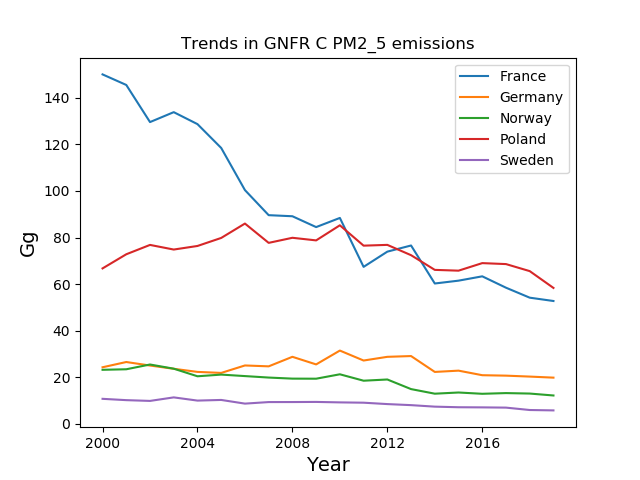
\includegraphics[width=12cm,trim=0 0 0 1.5cm,clip]{FIGS_TRENDS/PlotEmisTrends_PM2_5.png}
    \caption{Trends in \pmfine emissions from GNFR C (mainly residential heating). Values in parentheses give relative trends (here linear regression slopes), for the periods 2000-2019 and 2010--2019.}
    \label{fig:gnfrCtrends}
\end{figure}

 

Unlike EC, the observed seasonal trends for OC (c.f. Fig.~\ref{fig:KEX1} are very variable, with strong (ca. 4~\%) reductions in the winter months (both DJF and SON), and apparently no change in summertime. As already noted, the individual sites show a great variation in even the sign of the calculated trends, though statistically the trends are not significant (c.f.Fig.~\ref{fig:OCarrows}. The lack of clear trend in summertime is not surprising. 
OC has a substantial influence from
natural sources, biogenic secondary organic aerosol (BSOA) and primary
biological aerosol particles (PBAP), which prevail in the growing season \citep[e.g.][]{Gelencser:CARB,Yttri2019}.
These biogenic emissions are not subject to abatement, but are very sensitive to meteorology, and thus summer-time OC trends are strongly influenced by year-to-year changes in meteorological conditions.

Anthropogenic OC emissions
are likely best represented by winter-time data, and in DJF the observed trend of -4~\%/yr for OC is rather similar to that found for EC (Tab.~\ref{tab:KEX2}). As
for EC, domestic heating is an important emission source 
%Increased emissions from domestic heating are seen
all over Europe in the heating season
\citep[e.g.][]{Yttri2019}, but especially where RWC is utilised.
%when the contribution from natural sources
%is low, and is generally assumed to be poorly abated, particularly
%or residential wood burning. Notably, the winter-time reduction in OC
%was similar to that of EC considering all sites, and a
At the Birkenes
Observatory the winter-time reduction in OC (-4.1~\%/yr) was only somewhat
lower than for EC (-6.4~\%/yr) and levoglucosan (-4.6~\%/yr).
\SKIP{
  Karl Espen - where are these numbers coming from? Different to those in Tab.~\ref{tab:BirkenesTrends}
}
These results also suggest
that abatement of residential wood burning emissions has been quite
effective for Europe in general, taking into account the considerations
made about the length of the time series and the Birkenes Observatory as
an indicator of European emissions (Sect.~\ref{ss:trendsEC}).  

The underprediction of the OC levels in wintertime seen in Figs.~\ref{fig:KEX1} should not be taken as a indication that the EMEP model itself is wrong, but is rather at least partly the result of the issues with missing `condensable' organics (Sect.~\ref{ss:IssuesECOC}). It has been demonstrated elsewhere that model results improve substantially when condensables are included \citep{DeniervanderGon2015,R2019:SVOC,R2020:SVOC}. Unfortunately, we do not yet have a time-series of condensable organic emissions with which to perform trend analysis, but we hope to address that within the context of a new MSC-W led project funded by the Nordic Council of Ministers.

\SKIP{
A pronounced influence of natural sources in areas
less perturbed by anthropogenic emissions, exemplified by Scandinavia,
is a possible explanation \citep{Bergstrom2012,Yttri2021}, although a
less successful abatement of anthropogenic sources cannot be excluded.
}

%%%%%%%%%%%%%%%%%%



\subsection{OC and EC fractions of PM}
\label{ss:OCECfrac}


\begin{figure}
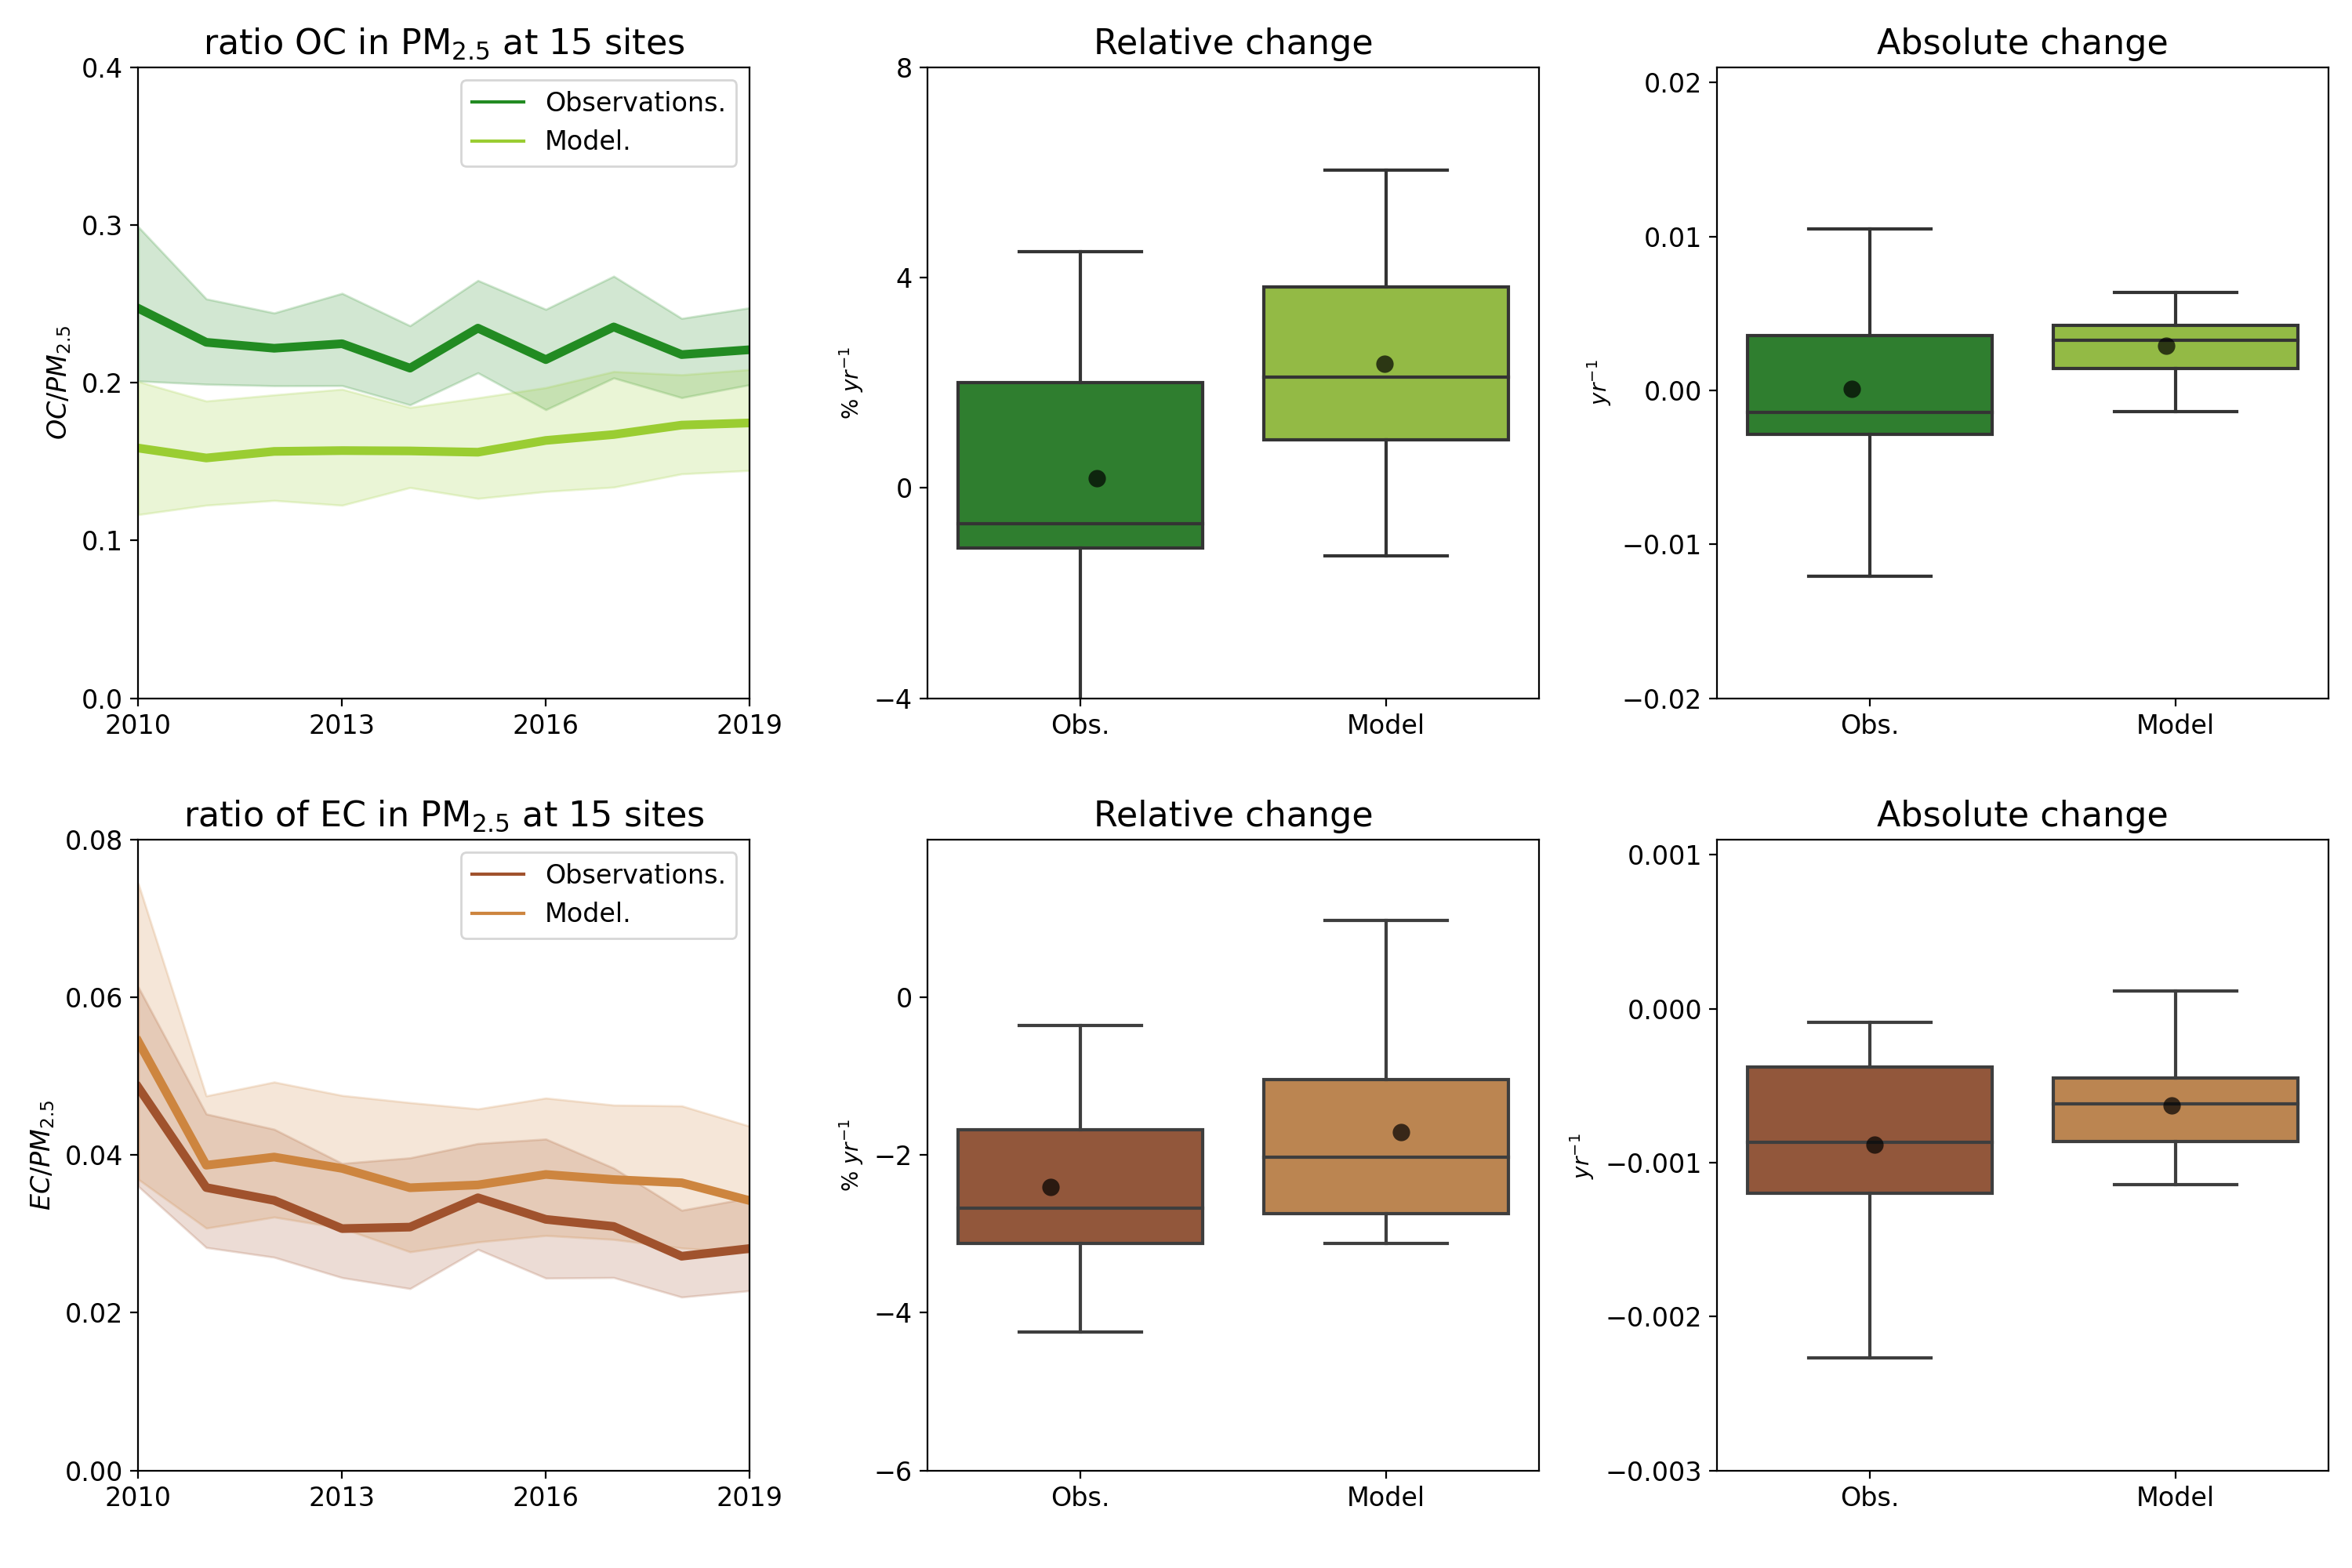
\includegraphics[width=16cm]{FIGS_TRENDS/ECOC_ratio_trends.png}
 \caption{Observed and modelled ratios and trends of OC/\pmfine and EC/\pmfine for
  15 EMEP sites across Europe for 2010--2019, showing the trends
  (left panels) of OC/\pmfine (upper) and EC (lower), aggregated annual and
  seasonal relative changes (mid panels) for OC (upper) and EC (lower),
  and aggregated annual and seasonal absolute changes (right panels)
  for OC (upper) and EC (lower). The solid line in the left panel shows
  the average annual mean for all sites and the shaded area the 95\%
  confidence interval. For explanation of the statistics in the figure,
  see Fig.~\label{fig:KEX3}
 }
\end{figure}

As focused abatement of anthropogenic secondary inorganic aerosol (SIA)
precursors have reduced ambient SIA levels substantially (Sects.~\ref{sec:Trends_sulfur}--\ref{sec:Trends_reduced nitrogen }), 
other, non-SIA fractions are likely to contribute an increasing fraction
of PM. For the EC fraction of \pmfine, however, there was a reduction,  -2.4$\pm$1.1~\%/yr, 
for 2010--2019 (Fig.~\ref{fig:KEX3}, Tab.~\ref{tab:KEX3}), showing that EC has been
more efficiently abated than the overall PM mass concentration. The model
calculated a comparable reduction (-1.7$\pm$1.3~\%/yr) for the EC/\pmfine ratio
but predicted a minor increase at two of the sites, which was not seen for
observed EC/\pmfine ratios. For the few sites where measurements allow for
a harmonized data set of EC, OC, \ce{SO4^2-} and \pmfine, i.e., only including
measurements on common days, the reduction in the EC fraction of \pmfine
was typically equally high or higher than for the \ce{SO4^2-} fraction. The
OC fraction of \pmfine showed no decrease or increase (0.2$\pm$2.8~\%/yr)
for 2010--2019 when considering all sites, which largely is explained by
non-abatable natural sources making up a major part of OC. A substantial
4.5~\%/yr increase in OC/\pmfine was calculated for the Norwegian sites,
experiencing low (anthropogenic) aerosol levels and a high OC fraction
from natural sources, thus one cannot exclude the possibility that part
of this increasing trend is due to an increase in natural sources and
not exclusively from a decrease in anthropogenic emissions. A 2.8~\%/yr
increase in the OC fraction was observed for the Spanish site Montseny,
resembling the Norwegian sites with respect to a low aerosol level and
a high OC fraction from natural sources \citep{Kulmala2011,Crippa2014}. For the
rest of continental Europe, a minor $\pm$1~\%/yr increase/decrease
was seen at most sites and a $\pm$2~\%/yr for a few. The Kosetice
(Czech Republic) (-5.3~\%/yr) and Shauinsland (Germany) (-3.1~\%/yr) sites
experienced a substantial decrease in the OC fraction, which was larger
than the corresponding decrease in the EC fraction, thus deviating from
the pattern seen at all other sites where the decrease in EC/\pmfine $>$
OC/\pmfine.

\begin{figure}
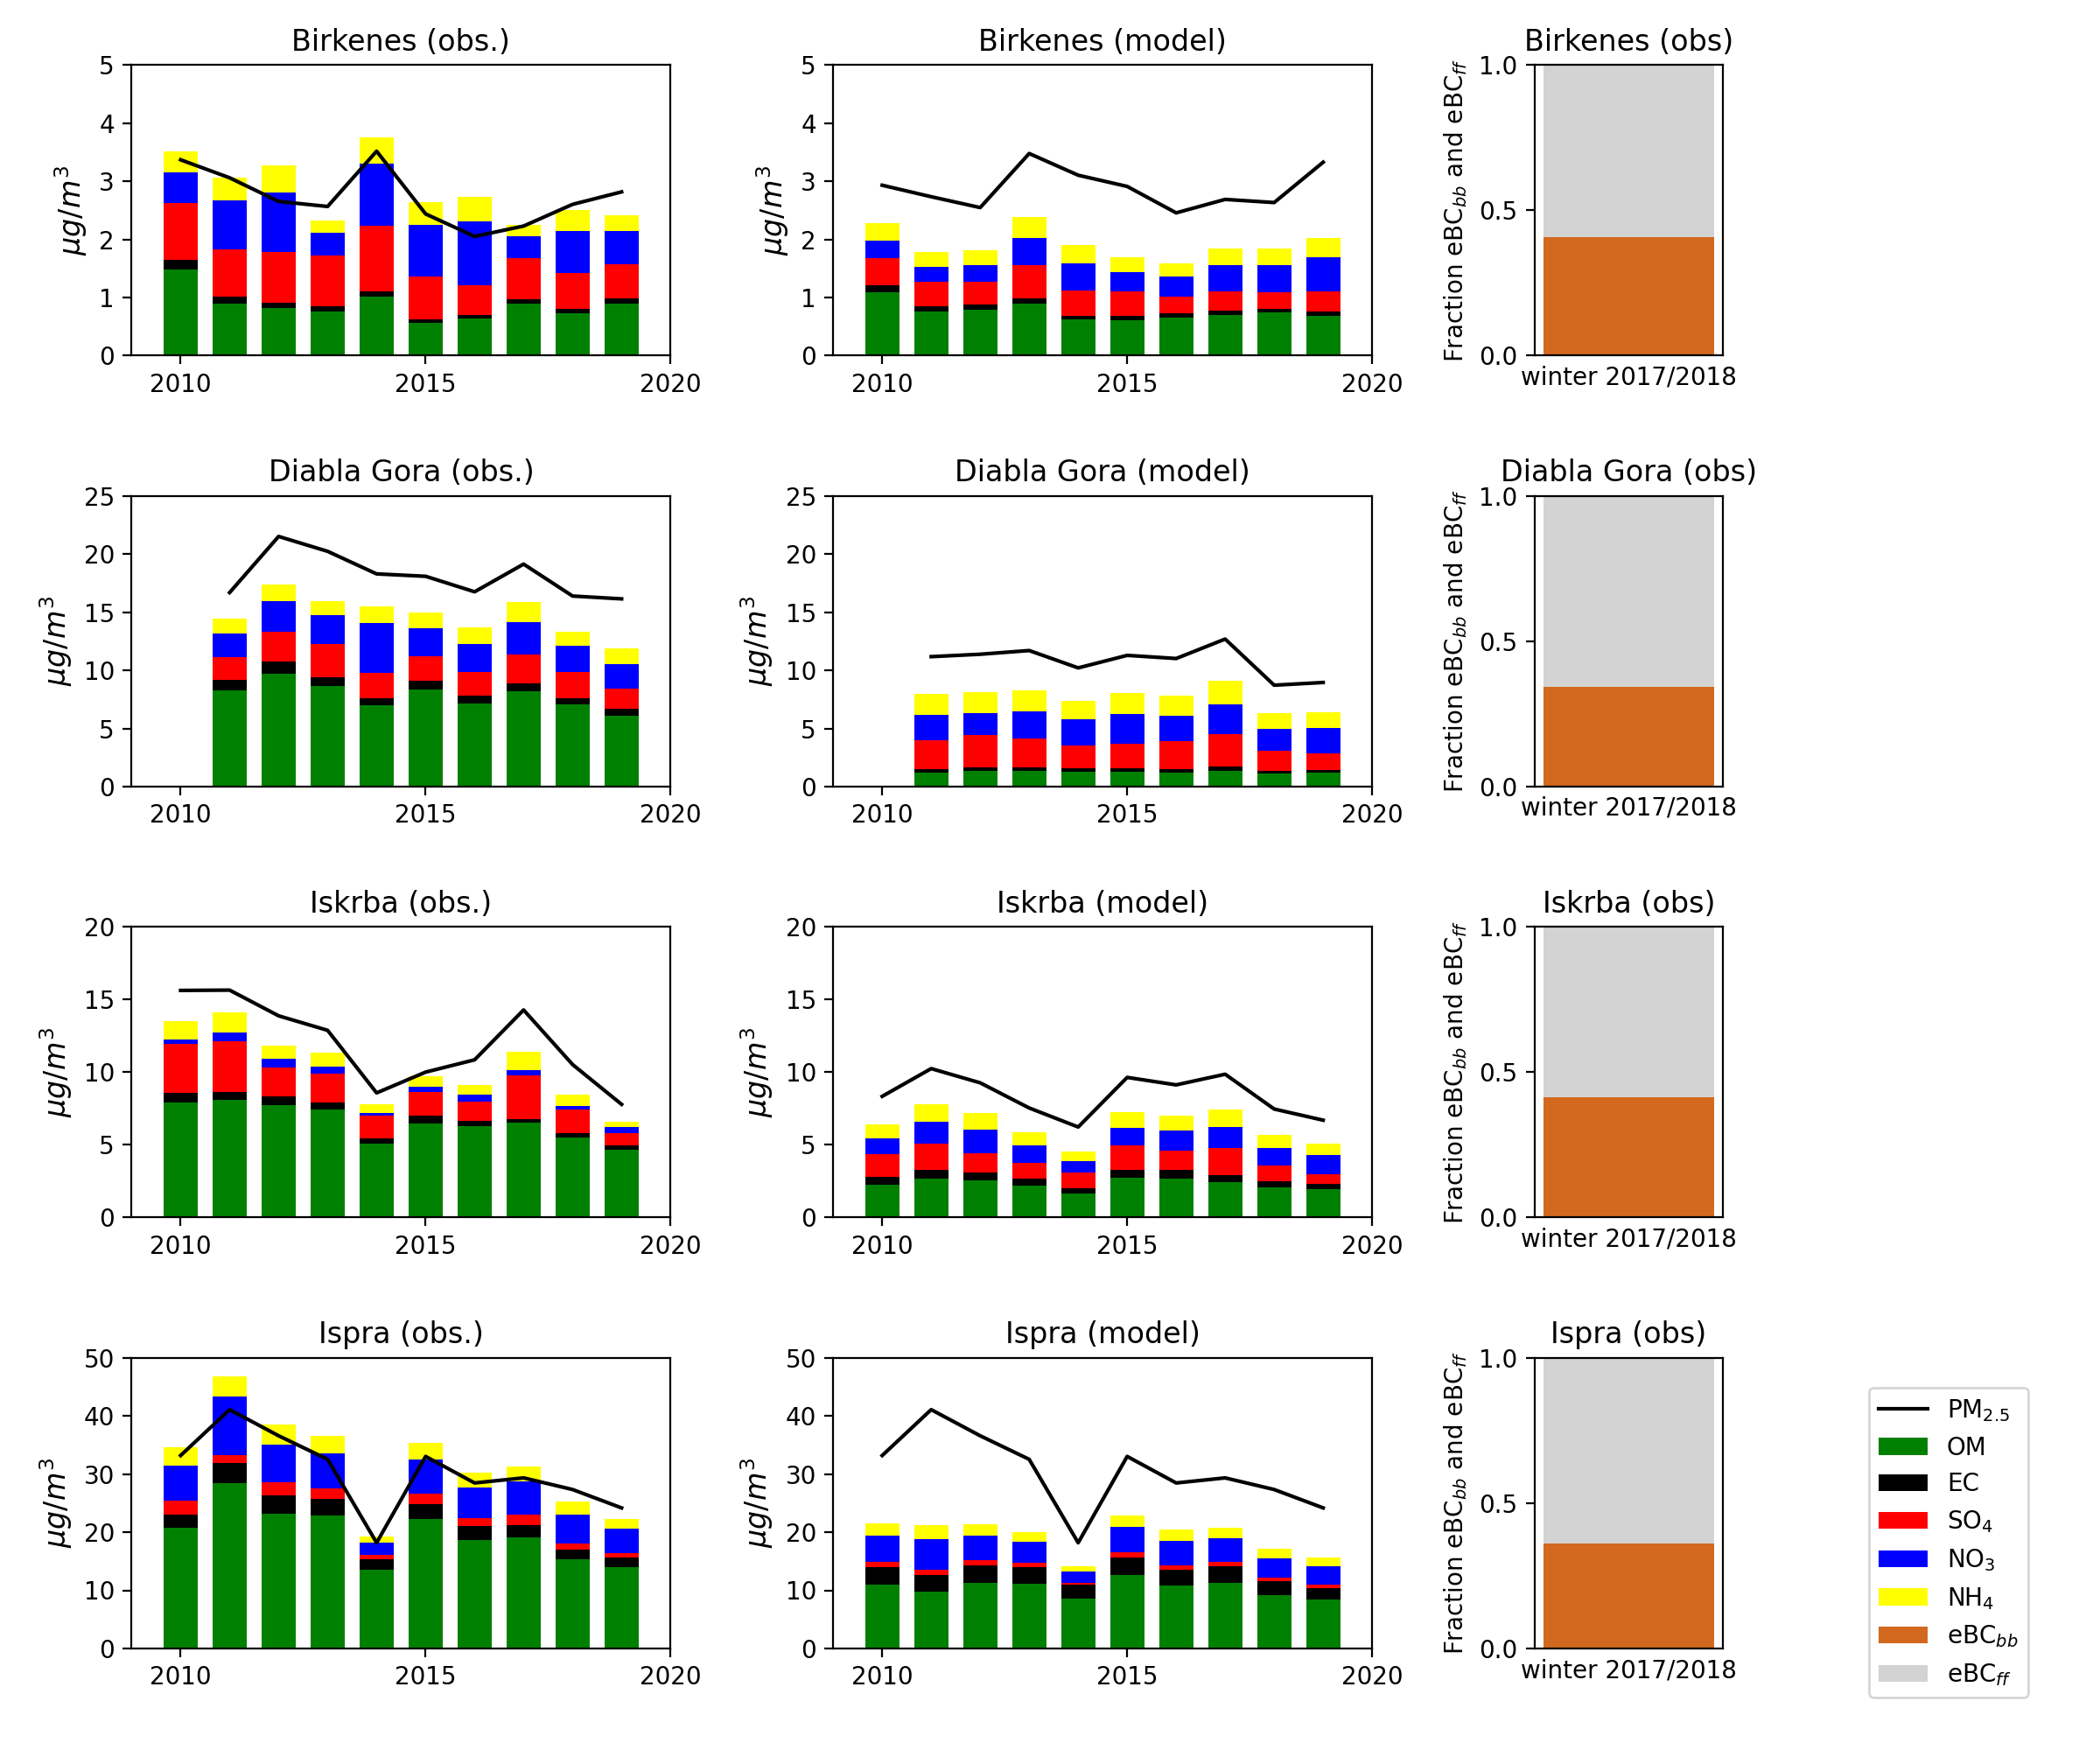
\includegraphics[width=16cm]{FIGS_TRENDS/Compostion_4sites_winter.png}
 \caption{
  Mass balance of wintertime \pmfine at  Birkenes (NO02), Diabla Gora
  (PL05), Iskrba (SI08) and Ispra (IT04) including OM, EC, \ce{SO4^2-}, \ce{NO3^-}, \ce{NH4^+} from 
  observations (left), modelled (middle) and apportionment of eBC
  into biomass burning/solid fuel (\EBCbb) and fossil fuel/liquid fuel
  (\EBCff) for winter 2017/2018 (right). Note that at NO02 and PLO5 the SIA components in observations are from filterpack sampler with no cutoff and thus probably overestimate the \pmfine SIA. \label{fig:KEX4}
 }
\end{figure}


The relative contribution of carbonaceous aerosol, OM (assuming OM = OC $\times$
1.4 for Ispra
\footnote{The lower factor is needed for Ispra to keep mass balance $\le$100\%.}
and 1.7 for the other sites)
 and EC, to the \pmfine mass concentration along with the major
SIA species illustrates the importance of the OM fraction for a further
reduction in wintertime \pmfine mass concentration (Fig.~\ref{fig:KEX4}). As a first step,
the natural and the anthropogenic fraction of the carbonaceous aerosol
must be separated, then further into abatable categories. Separation of
eBC into biomass burning/solid fuel (\EBCbb) and fossil fuel/liquid fuel
(\EBCff) is possible using data from the multi wavelength aethalometer,
currently available at $<$25 EMEP/ACTRIS sites across Europe \citep{Yttri:2014,Platt:2020a,Platt:2020b,Platt20XX}. An obvious next
step is to implement such analysis as part of regular monitoring,
making it possible to validate not only model performance, but also the
effort made in reducing carbonaceous aerosol from fossil fuel and biomass
burning sources. Although not directly comparable to the multi-year plots
presented in Fig.~\ref{fig:KEX4}, results from the EIMPs Winter 2017/2018 nicely
illustrates the split between \EBCbb and \EBCff for winter 2017/2018 for
the Italian site Ispra, (IT04), the Norwegian site Birkenes (NO02), the
Polish site Diabla Gora (PL05) and the Slovenian site Iskrba (SI08). The
apportionment of eBC can also be used to infer the corresponding fractions
of OM.

\begin{table}
\centering
\parbox{14cm}{
 \caption{
   Absolute and relative change and the corresponding 95\% confidence intervals in observed and modelled annual and seasonal    aggregated OC/\pmfine and EC/\pmfine ratios at 15 sites across Europe
   for 2010--2019. The number of sites with a significant outcome is provided.\label{tab:KEX3}
 }}
 \scalebox{0.95}{%
 \begin{tabular}{lcccccc}
\hline  % toprule
 &  &  &  &  &  &  \\
\multicolumn{7}{c}{EC/\pmfine (2010--2019)} \\
  &  &  &  &  &  &  \\
  \hline
     \multicolumn{3}{c}{Number of sites} & \multicolumn{2}{l}{Absolute change (\ugC/yr)} & \multicolumn{2}{l}{Relative change (\%/yr)} \\
{} &           total & sign. &                     abs &       Conf. interv. &                      \%/y &   Conf. interv. \\
%How   &                 &       &                         &                     &                          &                 \\
\hline  % midrule
Model &              15 &     5 &                 -0.0006 &  (-0.0009, -0.0004) &                    -1.71 &   (-2.32, -1.1) \\
Obs.  &              15 &     4 &                 -0.0009 &  (-0.0012, -0.0006) &                    -2.41 &  (-2.96, -1.85) \\
\hline  % bottomrule
% \end{tabular}
   &  &  &  &  &  &  \\
\multicolumn{7}{c}{OC/\pmfine (2010--2019)} \\
   &  &  &  &  &  &  \\
% \begin{tabular}{lrrrlrl}
\toprule
   \multicolumn{3}{c}{Number of sites} & \multicolumn{2}{l}{Absolute change (\ugC/yr)r} & \multicolumn{2}{l}{Relative change (\%/yr)} \\
{} &           total & sign. &                     abs &     Conf. interv. &                      \%/y &  Conf. interv. \\
%How   &                 &       &                         &                   &                          &                \\
\hline  % midrule
Model &              15 &     7 &                  0.0029 &   (0.0018, 0.004) &                     2.35 &     (1.3, 3.4) \\
Obs.  &              15 &     2 &                  0.0001 &  (-0.003, 0.0032) &                     0.19 &  (-1.24, 1.62) \\
\hline  % bottomrule
\end{tabular}
} % end scalebox
\end{table}




\subsection{Trends in EC and OC, conclusions}
\label{ss:trendsECOCconc}

For EC and OC we have calculated observed and modelled trends for 15 sites across Europe for the period 2010--2019. It should be noted that this 10-year period is rather short for the calculation of robust trends (and we show that slightly different time-windows produce different statistics), and typically only a limited number of sites showed trends that were statistically significant for specific seasons, even for a specific time-window. However, some features of the trend analysis seem rather consistent, and we summarise the main points here. 

A reduction (of ca. 4.5~\%/yr) in observed EC was found across 15 sites across Europe for the  period 
2010--2019. The reduction in levoglucosan at the site Birkenes in southern Norway (which is significantly impacted by long-range transport of pollution from continental Europe) was found to be over 5\% also (though this number was very sensitive to the time-window), which suggests that emissions from residential wood combustion were reduced significantly over this period; this is also consistent with reported changes in the GNFR C emissions from some countries at least. However, observed EC reduction levels were rather similar in all seasons, which suggests that emissions abatement of EC has been successful across a range of emission sources. 

In the winter season (DJF), reductions in observed EC and OC were very similar, with \mbox{-4.3~\%/yr} and -4.2~\%/yr respectively. Given that the winter OC concentrations are mainly determined by primary emissions and with minimal SOA contributions, this consistency of EC and OC reductions is also consistent with reductions in wintertime anthropogenic sources. Trends in observed OC in other seasons were however very mixed, with some stations showing increases, and others decreases, and with little statistical significance. This variability in station-to-station OC trends in other seasons reflects increasing contributions from SOA formation, which are sensitive to meteorological factors and biogenic emissions.

The modelled trends in EC (reduction of ca. 4~\%/yr) were rather similar to the observed trends, also across all seasons, and the station-mean EC concentrations themselves were well reproduced by the model across the 10 year period. 
For OC, the model substantially underpredicts the yearly concentrations over the whole period, and also underpredicts the trends.  

The underprediction of OC may partly be due to general difficulties with modelling SOA formation, but a major problem is the omission of condensable organics in the reported \pmfine emissions from many countries (Sect.~\ref{ss:IssuesECOC}). Although emissions estimates which include condensables (the so-called REF2 or REF2.1, Sect.~\ref{sec:EmisSVOC}) are available and were used in the status and source-receptor calculations of this report, these emissions only exist for 2015; no time-series of REF2-type emissions yet exists. The lack of significance of the calculated OC trends may also be attributed to some extent to these problems with condensables. When some countries include, and some exclude, condensables, changes in modelled OC concentrations will be very sensitive to changes in the source areas for the primary OC emissions entering the model.
Although modelling of EC is also impacted by the problems with condensables (due to the use of OC/EC ratios when interpreting \pmfine emission speciation, see Sect.~\ref{ss:IssuesECOC}), the much better agreement found for wintertime EC levels than for OC probably reflects the fact that EC has a wider variety of emission sources in that season (e.g. vehicles) than OC, which is much more dominated by residential wood-burning.


The EC fraction of \pmfine  decreased at all
sites (average of -2.4$\pm$1.1~\%/yr), and at a level equal to, or higher than, the \ce{SO4^2-} fraction. The
change in OC fraction was more scattered with a substantial and
consistent 4.5~\%/yr increase at the northernmost sites, whereas
there was no increase or decrease (0.2$\pm$2.8~\%/yr) when considering
all sites. The influence of OC from natural sources likely has a profound
impact on the general lack of decrease observed for the OC fraction of
\pmfine. These observations points to a continuous change in the aerosol
chemical composition and in the relative source composition across
Europe. The carbonaceous fraction appears particularly important for a
further reduction in the observed \pmfine mass concentration in Europe,
although effort is needed to separate its natural and anthropogenic
fraction to get a quantitative overview of the abatable fractions.
\\
\bigskip


\SKIP{ % COMMENT{\bigskip ORIG TEXT, DELETE if above is okay:\\}

A -4.5$\pm$1.6~\%/yr reduction in EC was calculated across Europe for
2010--2019 and the reduction was particularly consistent amongst the
sites where the reduction was statistically significant. The model
predicted a reduction that was somewhat lower (-3.9~\%/yr) than the
observations, but still comparable. A similar reduction in EC (-4.2~\%/yr)
was calculated for 2010--2019 as for 2001--2018 at the Birkenes
Observatory in southern Norway. This consistent reduction indicates a
potential for further reduction in future years for Europe in general,
as LRT from continental Europe explains most EC from both fossil fuel
and biomass burning sources at the Birkenes Observatory. A  -5.2~\%/yr
reduction in levoglucosan at the Birkenes Observatory (2010--2019)
 indicate that EC from wood burning in Europe is declining equally
rapid as that of EC from fossil fuel sources.

The reduction in OC (-2.4$\pm$1.6~\%/yr) was less pronounced than for EC,
whereas winter-time levels (-4.2~\%/yr) were comparable to EC. Non-abatable
natural sources of OC peak in the growing season diluting anthropogenic
sources, thus, anthropogenic OC emissions are likely best represented by
winter-time data. Comparable reductions in winter-time OC (-4.1~\%/yr),
winter-time EC (-6.4~\%/yr) and winter-time levoglucosan (-4.6~\%/yr)
at the Birkenes Observatory suggest that abatement of residential
wood burning emissions has been quite effective for Europe in general,
taking into account considerations about the length of the time series
and Birkenes as an indicator of European emissions.

The model calculated a reduction in OC of -0.6~\%/yr, being noticeable
less than for the observations (-2.4~\%/yr). A similar underprediction
was seen for each season, thereby reproducing the seasonality in trend
seen for the observations.

The EC fraction of \pmfine decreased at all
sites (-2.4$\pm$1.1~\%/yr), and at a level equal to, or higher than, the \ce{SO4^2-} fraction. The
change in OC fraction was more scattered with a substantial and
consistent 4.5~\%/yr increase at the northernmost sites, whereas
there was no increase or decrease (0.2$\pm$2.8~\%/yr) when considering
all sites. Influence of OC from natural sources likely has a profound
impact on the general lack of decrease observed for the OC fraction of
\pmfine. These observations points to a continuous change in the aerosol
chemical composition and in the relative source composition across
Europe. The carbonaceous fraction appears particularly important for a
further reduction in the observed \pmfine mass concentration in Europe,
although effort is needed to separate its natural and anthropogenic
fraction to get a quantitative overview of the abatable fractions.\\
}


\SKIP{ % Now moved to ExecSummary
For EC and OC we have calculated observed and modelled trends for 15 sites across Europe for the period 2010--2019. A reduction (of ca. 4.5~\%/yr) in observed EC was found, and a similar reduction was found for OC in the winter months (when OC is expected to be most sensitive to primary anthropogenic emissions rather than to OA associated with biogenic sources). These trends suggest that abatement measures are having some success in reducing both EC and OC in Europe, especially in wintertime.  The model reproduced modelled EC values and trends quite well, but underpredicted OC, both in terms of absolute values and trends. This underprediction is at least partly due to the omission of condensable organics in the reported emissions from many countries. 
%
The carbonaceous fraction appears particularly important for a
further reduction in the observed \pmfine mass concentration in Europe,
although effort is needed to separate its natural and anthropogenic
fraction to get a quantitative overview of the abatable fractions.
}


\clearpage
\section{Exceedances of critical loads of acidification and eutrophication in 2000 to 2019.}
\label{subs:exceedSnN}
%Thomas/CCE: I just updated this section. Please have a look TS 17.08.2021

The exceedances of European critical loads (CLs) are computed for the total nitrogen
(N) and sulphur (S) depositions modelled on the 0.1$\degrees \times$ 0.1$\degrees$
longitude-latitude grid (approx. 11 x 5.5 km$^{2}$ at 60$\degrees$N).
Exceedances are calculated for the European critical loads documented in \cite{Hettelingh:2017}, while
a description of the methods is given in \cite{DeVries:2015}. The
critical loads data for eutrophication by N (CL eut N) and for acidification by N and S
(CL acid) are also used by the EMEP Centre CIAM (located at IIASA) in their integrated assessment
modelling. The exceedance in a grid cell is the so-called ’average accumulated
exceedance’ (AAE), which is calculated as the area-weighted average of the
exceedances of the critical loads of all ecosystems in this grid cell. The units for
critical loads and their exceedances are equivalents (eq; same as \textit{moles of charge},
molc) per area and time, making S and N depositions comparable on their impacts, which is important for
acidity CLs.

Critical loads are available for about 4 million ecosystems in Europe covering an area
of about 3 million km$^{2}$ (west of 42$\degrees$E). The exceedances (AAE) of those critical loads
are computed on a 0.1$\degrees \times$ 0.1$\degrees$ longitude-latitude grid, and maps for the deposition in
the years 2000, 2005, 2010, 2015 and 2019 are shown in Figures \ref{fig:eutN} and \ref{fig:acid}. As indicated in the maps, the critical loads for eutrophication are exceeded in practically all countries in all years. The share of ecosystems where the critical load for eutrophication is exceeded decreases relatively slowly, starting at 76.4\% in 2000 and ending at 65.5\% in 2019.
European average AAE is about 452 eq ha$^{-1}$ yr$^{-1}$ (2000) and 276 eq
ha$^{-1}$ yr$^{-1}$ (2019). The highest exceedances of CLs are found in the Po Valley in Italy, the
Dutch-German-Danish border areas and in north-eastern Spain.
By contrast, critical loads of acidity are exceeded in a much smaller area. Hot spots of
exceedances can be found in the Netherlands and its border areas to Germany and
Belgium, and some smaller maxima in southern Germany and Czechia,
whereas most of Europe is not exceeded (grey areas). Acidity exceedances occur
on 16.2\% (2000) and 5.0\% (2019) of the ecosystem area and the European average
AAE is about 133 eq ha$^{-1}$ yr$^{-1}$ (2000) and 25 eq ha$^{-1}$ yr$^{-1}$ (2019). Overall statistics for the share of critical load exceedance and European average of AAE are shown in Figures \ref{fig:stats_cl_ex}.
\begin{figure}[ht]
  \centering
  \subfigure{\includegraphics*[scale=0.20]{FIGS_CL_Exceedance/Stats_CLex_eut.png}}
  \subfigure{\includegraphics*[scale=0.20]{FIGS_CL_Exceedance/Stats_CLex_acid.png}}
  \caption{Summary for exceedance of critical load for eutrophication (left) and acidification (right).}
\label{fig:stats_cl_ex}
\end{figure}
\begin{figure}[ht]
  \centering
  \subfigure{\includegraphics*[scale=0.35]{FIGS_CL_Exceedance/CL_Ex_eut_2000.png}}
  \subfigure{\includegraphics*[scale=0.35]{FIGS_CL_Exceedance/CL_Ex_eut_2005.png}}
  \subfigure{\includegraphics*[scale=0.35]{FIGS_CL_Exceedance/CL_Ex_eut_2010.png}}
  \subfigure{\includegraphics*[scale=0.35]{FIGS_CL_Exceedance/CL_Ex_eut_2015.png}}
  \subfigure{\includegraphics*[scale=0.35]{FIGS_CL_Exceedance/CL_Ex_eut_2019.png}}
 \caption{Exceedance of critical load for eutrophication for the years 2000, 2005, 2010, 2015 and 2019.}
\label{fig:eutN}
\end{figure}
\begin{figure}[ht]
  \centering
 \subfigure{\includegraphics*[scale=0.35]{FIGS_CL_Exceedance/CL_Ex_acid_2000.png}}
  \subfigure{\includegraphics*[scale=0.35]{FIGS_CL_Exceedance/CL_Ex_acid_2005.png}}
  \subfigure{\includegraphics*[scale=0.35]{FIGS_CL_Exceedance/CL_Ex_acid_2010.png}}
  \subfigure{\includegraphics*[scale=0.35]{FIGS_CL_Exceedance/CL_Ex_acid_2015.png}}
  \subfigure{\includegraphics*[scale=0.35]{FIGS_CL_Exceedance/CL_Ex_acid_2019.png}}
 \caption{Exceedance of critical load for acidification for the years 2000, 2005, 2010, 2015 and 2019.}
\label{fig:acid}
\end{figure}





%%%%%%%%%%%%%%%%%%%%%%%%%%%%%%%%%%%%%%%%%%%%%%%%%%%%%%%%%%%%%%%%%%%%%%%%%%%%%%%%%%%%%%
\clearpage


\bibliographystyle{copernicus}         % change bibliography-name after each
\renewcommand\bibname{References}      % bibliographystyle command!
\addcontentsline{toc}{section}{References}
%\bibliography{trends,Refs,EMEP_Reports,NILU,RefsUpdates,RefsEmis}
\bibliography{Refs2021}
